%% fig_closure.tex   (generated by make_closure.py; do not edit by hand)
%% The implication graph of the scope section: the spine of derived statements, the open statements at the level where each is needed, and the propagation statement with its three constraints.
\documentclass[tikz,border=8pt]{standalone}
\usepackage{amsmath,amssymb}
\usetikzlibrary{arrows.meta,calc}
%% palette.tex -- shared colour definitions for the figures
\definecolor{PInk}{RGB}{26,32,44}
\definecolor{PBlue}{RGB}{37,82,139}
\definecolor{PTeal}{RGB}{23,127,125}
\definecolor{POchre}{RGB}{193,138,44}
\definecolor{PClay}{RGB}{178,74,58}
\definecolor{PSlate}{RGB}{108,122,137}
\definecolor{PViolet}{RGB}{110,86,150}
\definecolor{WBlue}{RGB}{223,234,246}
\definecolor{WTeal}{RGB}{220,238,236}
\definecolor{WOchre}{RGB}{250,240,218}
\definecolor{WClay}{RGB}{247,229,224}
\definecolor{WSlate}{RGB}{238,241,244}
\definecolor{PMag}{RGB}{158,58,110}
\definecolor{PGrass}{RGB}{62,124,66}
\definecolor{PAmber}{RGB}{214,112,38}
\definecolor{PIndigo}{RGB}{58,64,140}
\definecolor{PRule}{RGB}{176,186,197}

%% shared macros so the standalone figures match the paper
\providecommand{\QQ}{\mathbb{Q}}
\providecommand{\ZZ}{\mathbb{Z}}
\providecommand{\RR}{\mathbb{R}}
\providecommand{\CC}{\mathbb{C}}
\providecommand{\PP}{\mathbb{P}}
\providecommand{\Kx}{K^{\times}}
\providecommand{\HW}{W}
\providecommand{\Nm}{\mathrm{N}}
\providecommand{\Hdg}{\mathrm{Hdg}}
\providecommand{\NS}{\mathrm{NS}}
\providecommand{\cA}{\mathcal{A}}
\providecommand{\cD}{\mathcal{D}}
\providecommand{\cF}{\mathcal{F}}
\providecommand{\cP}{\mathcal{P}}
\providecommand{\cO}{\mathcal{O}}
\providecommand{\cQ}{\mathcal{Q}}
\providecommand{\bbar}[1]{\overline{#1}}
\providecommand{\ch}{\operatorname{ch}}
\providecommand{\End}{\mathrm{End}}

\begin{document}
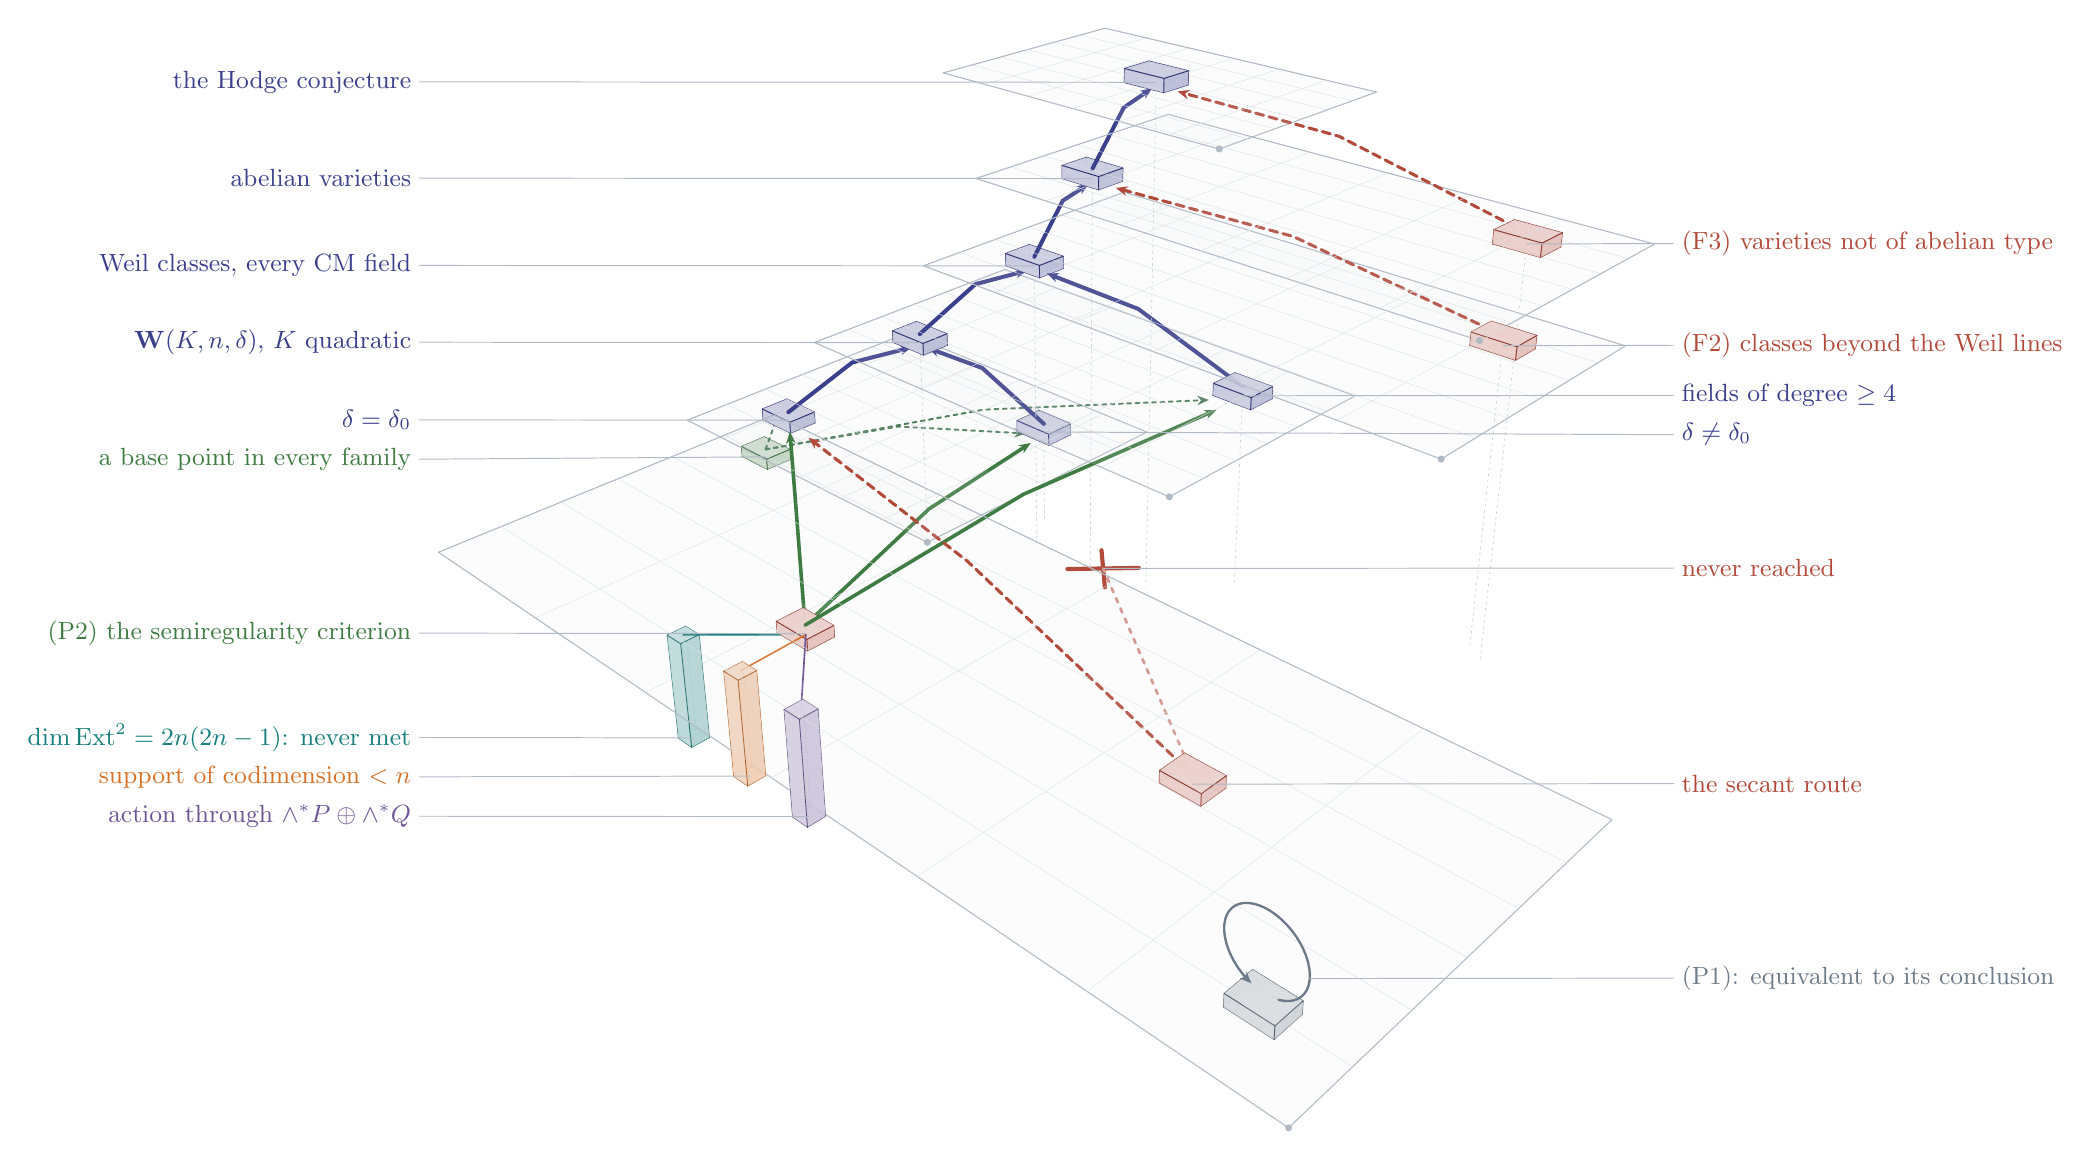
\begin{tikzpicture}[x=1cm,y=1cm,line join=round,line cap=round,
  font=\small,text=PInk]
  \path[draw=none,fill opacity=0.12,fill=PSlate!16!white] (-4.1723,-0.6797) -- (-3.5447,-0.9927) -- (-3.1261,-0.8128) -- (-3.7553,-0.5090) -- cycle;
  \path[draw=none,fill opacity=0.12,fill=PSlate!16!white] (-2.3547,0.4155) -- (-2.1253,0.3193) -- (-1.8425,0.4333) -- (-2.0720,0.5275) -- cycle;
  \draw[PGrass!80!black,line width=0.35pt] (-3.8643,-0.9120) -- (-3.8741,-0.7874);
  \path[draw=none,fill opacity=0.12,fill=PSlate!16!white] (-4.6019,-0.8555) -- (-3.9763,-1.1782) -- (-3.5447,-0.9927) -- (-4.1723,-0.6797) -- cycle;
  \path[draw=none,fill opacity=0.12,fill=PSlate!16!white] (-2.1253,0.3193) -- (-1.8917,0.2214) -- (-1.6089,0.3375) -- (-1.8425,0.4333) -- cycle;
  \draw[PGrass!80!black,line width=0.35pt] (-4.1557,-1.0350) -- (-3.8643,-0.9120);
  \path[draw=none,fill opacity=0.12,fill=PSlate!16!white] (-2.6435,0.3011) -- (-2.4143,0.2028) -- (-2.1253,0.3193) -- (-2.3547,0.4155) -- cycle;
  \path[draw=none,fill opacity=0.88,fill=PGrass!34!white] (-4.1557,-1.0350) -- (-3.8643,-0.9120) -- (-3.8741,-0.7874) -- (-4.1664,-0.9094) -- cycle;
  \draw[PGrass!80!black,line width=0.35pt] (-3.8643,-0.9120) -- (-3.5447,-1.0725);
  \draw[PGrass!80!black,line width=0.35pt] (-4.1664,-0.9094) -- (-3.8741,-0.7874);
  \path[draw=none,fill opacity=0.88,fill=PGrass!27!white] (-3.8643,-0.9120) -- (-3.5447,-1.0725) -- (-3.5538,-0.9466) -- (-3.8741,-0.7874) -- cycle;
  \draw[PGrass!80!black,line width=0.35pt] (-3.8741,-0.7874) -- (-3.5538,-0.9466);
  \draw[PGrass!80!black,line width=0.35pt] (-4.1557,-1.0350) -- (-4.1664,-0.9094);
  \path[draw=none,fill opacity=0.88,fill=PGrass!25!white] (-4.1557,-1.0350) -- (-3.8367,-1.1988) -- (-3.5447,-1.0725) -- (-3.8643,-0.9120) -- cycle;
  \path[draw=none,fill opacity=0.12,fill=PSlate!16!white] (-1.8917,0.2214) -- (-1.6538,0.1216) -- (-1.3709,0.2398) -- (-1.6089,0.3375) -- cycle;
  \path[draw=none,fill opacity=0.12,fill=PSlate!16!white] (-3.5447,-0.9927) -- (-2.8825,-1.3230) -- (-2.4627,-1.1331) -- (-3.1261,-0.8128) -- cycle;
  \path[draw=none,fill opacity=0.88,fill=PGrass!25!white] (-4.1664,-0.9094) -- (-3.8466,-1.0720) -- (-3.5538,-0.9466) -- (-3.8741,-0.7874) -- cycle;
  \draw[PGrass!80!black,line width=0.35pt] (-3.5447,-1.0725) -- (-3.5538,-0.9466);
  \path[draw=none,fill opacity=0.12,fill=PSlate!16!white] (-2.4143,0.2028) -- (-2.1808,0.1027) -- (-1.8917,0.2214) -- (-2.1253,0.3193) -- cycle;
  \path[draw=none,fill opacity=0.12,fill=PSlate!16!white] (-2.9386,0.1842) -- (-2.7096,0.0837) -- (-2.4143,0.2028) -- (-2.6435,0.3011) -- cycle;
  \draw[PGrass!80!black,line width=0.35pt] (-4.1557,-1.0350) -- (-3.8367,-1.1988);
  \path[draw=none,fill opacity=0.12,fill=PSlate!16!white] (-5.0447,-1.0368) -- (-4.4215,-1.3695) -- (-3.9763,-1.1782) -- (-4.6019,-0.8555) -- cycle;
  \path[draw=none,fill opacity=0.88,fill=PGrass!27!white] (-4.1557,-1.0350) -- (-3.8367,-1.1988) -- (-3.8466,-1.0720) -- (-4.1664,-0.9094) -- cycle;
  \draw[PGrass!80!black,line width=0.35pt] (-3.8367,-1.1988) -- (-3.5447,-1.0725);
  \draw[PGrass!80!black,line width=0.35pt] (-4.1664,-0.9094) -- (-3.8466,-1.0720);
  \path[draw=none,fill opacity=0.88,fill=PGrass!34!white] (-3.8367,-1.1988) -- (-3.5447,-1.0725) -- (-3.5538,-0.9466) -- (-3.8466,-1.0720) -- cycle;
  \draw[PGrass!80!black,line width=0.35pt] (-3.8466,-1.0720) -- (-3.5538,-0.9466);
  \path[draw=none,fill opacity=0.12,fill=PSlate!16!white] (-1.6538,0.1216) -- (-1.4114,0.0199) -- (-1.1286,0.1404) -- (-1.3709,0.2398) -- cycle;
  \path[draw=none,fill opacity=0.12,fill=PSlate!16!white] (-2.1808,0.1027) -- (-1.9429,0.0007) -- (-1.6538,0.1216) -- (-1.8917,0.2214) -- cycle;
  \draw[PGrass!80!black,line width=0.35pt] (-3.8367,-1.1988) -- (-3.8466,-1.0720);
  \path[draw=none,fill opacity=0.12,fill=PSlate!16!white] (-2.7096,0.0837) -- (-2.4763,-0.0186) -- (-2.1808,0.1027) -- (-2.4143,0.2028) -- cycle;
  \path[draw=none,fill opacity=0.12,fill=PSlate!16!white] (-3.2403,0.0647) -- (-3.0116,-0.0380) -- (-2.7096,0.0837) -- (-2.9386,0.1842) -- cycle;
  \path[draw=none,fill opacity=0.12,fill=PSlate!16!white] (-3.9763,-1.1782) -- (-3.3157,-1.5189) -- (-2.8825,-1.3230) -- (-3.5447,-0.9927) -- cycle;
  \path[draw=none,fill opacity=0.12,fill=PSlate!16!white] (-1.4114,0.0199) -- (-1.1645,-0.0836) -- (-0.8818,0.0391) -- (-1.1286,0.1404) -- cycle;
  \path[draw=none,fill opacity=0.12,fill=PSlate!16!white] (-5.5012,-1.2236) -- (-4.8809,-1.5669) -- (-4.4215,-1.3695) -- (-5.0447,-1.0368) -- cycle;
  \path[draw=none,fill opacity=0.12,fill=PSlate!16!white] (-1.9429,0.0007) -- (-1.7006,-0.1032) -- (-1.4114,0.0199) -- (-1.6538,0.1216) -- cycle;
  \path[draw=none,fill opacity=0.12,fill=PSlate!16!white] (-2.4763,-0.0186) -- (-2.2386,-0.1229) -- (-1.9429,0.0007) -- (-2.1808,0.1027) -- cycle;
  \path[draw=none,fill opacity=0.12,fill=PSlate!16!white] (-3.0116,-0.0380) -- (-2.7785,-0.1427) -- (-2.4763,-0.0186) -- (-2.7096,0.0837) -- cycle;
  \path[draw=none,fill opacity=0.12,fill=PSlate!16!white] (-3.5487,-0.0575) -- (-3.3203,-0.1625) -- (-3.0116,-0.0380) -- (-3.2403,0.0647) -- cycle;
  \path[draw=none,fill opacity=0.12,fill=PSlate!16!white] (-1.1645,-0.0836) -- (-0.9128,-0.1891) -- (-0.6303,-0.0641) -- (-0.8818,0.0391) -- cycle;
  \path[draw=none,fill opacity=0.12,fill=PSlate!16!white] (-2.8825,-1.3230) -- (-2.1828,-1.6720) -- (-1.7623,-1.4712) -- (-2.4627,-1.1331) -- cycle;
  \path[draw=none,fill opacity=0.12,fill=PSlate!16!white] (-1.0700,1.2434) -- (-0.7481,1.1250) -- (-0.5009,1.2222) -- (-0.8226,1.3383) -- cycle;
  \path[draw=none,fill opacity=0.12,fill=PSlate!16!white] (-1.7006,-0.1032) -- (-1.4536,-0.2092) -- (-1.1645,-0.0836) -- (-1.4114,0.0199) -- cycle;
  \path[draw=none,fill opacity=0.12,fill=PSlate!16!white] (-2.2386,-0.1229) -- (-1.9963,-0.2292) -- (-1.7006,-0.1032) -- (-1.9429,0.0007) -- cycle;
  \path[draw=none,fill opacity=0.12,fill=PSlate!16!white] (-4.4215,-1.3695) -- (-3.7628,-1.7212) -- (-3.3157,-1.5189) -- (-3.9763,-1.1782) -- cycle;
  \path[draw=none,fill opacity=0.12,fill=PSlate!16!white] (-2.7785,-0.1427) -- (-2.5409,-0.2494) -- (-2.2386,-0.1229) -- (-2.4763,-0.0186) -- cycle;
  \path[draw=none,fill opacity=0.12,fill=PSlate!16!white] (-3.3203,-0.1625) -- (-3.0875,-0.2696) -- (-2.7785,-0.1427) -- (-3.0116,-0.0380) -- cycle;
  \draw[PGrass!70!PSlate,line width=0.70pt,dash pattern=on 1.4pt off 1.6pt,-{Stealth[length=4.2pt,width=3.4pt]}] (-3.8591,-0.9469) -- (-3.7299,-0.5841) -- (-3.5812,-0.6042);
  \path[draw=none,fill opacity=0.12,fill=PSlate!16!white] (-5.9722,-1.4164) -- (-5.3552,-1.7708) -- (-4.8809,-1.5669) -- (-5.5012,-1.2236) -- cycle;
  \path[draw=none,fill opacity=0.12,fill=PSlate!16!white] (-3.8641,-0.1824) -- (-3.6361,-0.2899) -- (-3.3203,-0.1625) -- (-3.5487,-0.0575) -- cycle;
  \path[draw=none,fill opacity=0.12,fill=PSlate!16!white] (-0.9128,-0.1891) -- (-0.6563,-0.2967) -- (-0.3740,-0.1692) -- (-0.6303,-0.0641) -- cycle;
  \path[draw=none,fill opacity=0.12,fill=PSlate!16!white] (-1.3224,1.1466) -- (-1.0004,1.0258) -- (-0.7481,1.1250) -- (-1.0700,1.2434) -- cycle;
  \path[draw=none,fill opacity=0.12,fill=PSlate!16!white] (-1.4536,-0.2092) -- (-1.2018,-0.3171) -- (-0.9128,-0.1891) -- (-1.1645,-0.0836) -- cycle;
  \draw[PRule!45,line width=0.15pt] (-4.3976,-0.8074) -- (-1.6089,0.3375);
  \path[draw=none,fill opacity=0.12,fill=PSlate!16!white] (-1.9963,-0.2292) -- (-1.7493,-0.3376) -- (-1.4536,-0.2092) -- (-1.7006,-0.1032) -- cycle;
  \path[draw=none,fill opacity=0.12,fill=PSlate!16!white] (-0.7481,1.1250) -- (-0.4184,1.0037) -- (-0.1714,1.1033) -- (-0.5009,1.2222) -- cycle;
  \draw[PGrass!70!PSlate,line width=0.70pt,dash pattern=on 1.4pt off 1.6pt,-{Stealth[length=4.2pt,width=3.4pt]}] (-3.8591,-0.9469) -- (-2.1745,-0.6559) -- (-0.5545,-0.7440);
  \path[draw=none,fill opacity=0.12,fill=PSlate!16!white] (-2.5409,-0.2494) -- (-2.2988,-0.3581) -- (-1.9963,-0.2292) -- (-2.2386,-0.1229) -- cycle;
  \draw[PRule!45,line width=0.15pt] (-2.4983,0.3586) -- (0.5612,-0.9387);
  \path[draw=none,fill opacity=0.12,fill=PSlate!16!white] (-3.3157,-1.5189) -- (-2.6169,-1.8792) -- (-2.1828,-1.6720) -- (-2.8825,-1.3230) -- cycle;
  \path[draw=none,fill opacity=0.12,fill=PSlate!16!white] (-3.0875,-0.2696) -- (-2.8503,-0.3787) -- (-2.5409,-0.2494) -- (-2.7785,-0.1427) -- cycle;
  \path[draw=none,fill opacity=0.12,fill=PSlate!16!white] (-3.6361,-0.2899) -- (-3.4037,-0.3994) -- (-3.0875,-0.2696) -- (-3.3203,-0.1625) -- cycle;
  \path[draw=none,fill opacity=0.12,fill=PSlate!16!white] (-0.6563,-0.2967) -- (-0.3948,-0.4064) -- (-0.1128,-0.2764) -- (-0.3740,-0.1692) -- cycle;
  \path[draw=none,fill opacity=0.12,fill=PSlate!16!white] (-4.8809,-1.5669) -- (-4.2247,-1.9301) -- (-3.7628,-1.7212) -- (-4.4215,-1.3695) -- cycle;
  \path[draw=none,fill opacity=0.12,fill=PSlate!16!white] (-4.1867,-0.3102) -- (-3.9592,-0.4202) -- (-3.6361,-0.2899) -- (-3.8641,-0.1824) -- cycle;
  \path[draw=none,fill opacity=0.12,fill=PSlate!16!white] (-1.2018,-0.3171) -- (-0.9452,-0.4272) -- (-0.6563,-0.2967) -- (-0.9128,-0.1891) -- cycle;
  \path[draw=none,fill opacity=0.12,fill=PSlate!16!white] (-1.5798,1.0478) -- (-1.2577,0.9246) -- (-1.0004,1.0258) -- (-1.3224,1.1466) -- cycle;
  \path[draw=none,fill opacity=0.12,fill=PSlate!16!white] (-1.7493,-0.3376) -- (-1.4975,-0.4480) -- (-1.2018,-0.3171) -- (-1.4536,-0.2092) -- cycle;
  \path[draw=none,fill opacity=0.12,fill=PSlate!16!white] (-1.0004,1.0258) -- (-0.6704,0.9020) -- (-0.4184,1.0037) -- (-0.7481,1.1250) -- cycle;
  \path[draw=none,fill opacity=0.12,fill=PSlate!16!white] (-6.4582,-1.6153) -- (-5.8452,-1.9813) -- (-5.3552,-1.7708) -- (-5.9722,-1.4164) -- cycle;
  \path[draw=none,fill opacity=0.12,fill=PSlate!16!white] (-2.2988,-0.3581) -- (-2.0519,-0.4690) -- (-1.7493,-0.3376) -- (-1.9963,-0.2292) -- cycle;
  \path[draw=none,fill opacity=0.12,fill=PSlate!16!white] (-0.4184,1.0037) -- (-0.0804,0.8794) -- (0.1663,0.9815) -- (-0.1714,1.1033) -- cycle;
  \path[draw=none,fill opacity=0.12,fill=PSlate!16!white] (-2.8503,-0.3787) -- (-2.6083,-0.4900) -- (-2.2988,-0.3581) -- (-2.5409,-0.2494) -- cycle;
  \path[draw=none,fill opacity=0.12,fill=PSlate!16!white] (-3.4037,-0.3994) -- (-3.1668,-0.5111) -- (-2.8503,-0.3787) -- (-3.0875,-0.2696) -- cycle;
  \path[draw=none,fill opacity=0.12,fill=PSlate!16!white] (-2.1828,-1.6720) -- (-1.4422,-2.0413) -- (-1.0218,-1.8288) -- (-1.7623,-1.4712) -- cycle;
  \path[draw=none,fill opacity=0.12,fill=PSlate!16!white] (-0.3948,-0.4064) -- (-0.1282,-0.5182) -- (0.1535,-0.3857) -- (-0.1128,-0.2764) -- cycle;
  \path[draw=none,fill opacity=0.12,fill=PSlate!16!white] (-3.9592,-0.4202) -- (-3.7273,-0.5322) -- (-3.4037,-0.3994) -- (-3.6361,-0.2899) -- cycle;
  \path[draw=none,fill opacity=0.12,fill=PSlate!16!white] (-0.9452,-0.4272) -- (-0.6835,-0.5394) -- (-0.3948,-0.4064) -- (-0.6563,-0.2967) -- cycle;
  \draw[PRule!45,line width=0.15pt] (-3.9219,-1.0496) -- (-1.1286,0.1404);
  \path[draw=none,fill opacity=0.12,fill=PSlate!16!white] (-1.8425,0.9470) -- (-1.5204,0.8213) -- (-1.2577,0.9246) -- (-1.5798,1.0478) -- cycle;
  \path[draw=none,fill opacity=0.12,fill=PSlate!16!white] (-4.5167,-0.4410) -- (-4.2899,-0.5535) -- (-3.9592,-0.4202) -- (-4.1867,-0.3102) -- cycle;
  \path[draw=none,fill opacity=0.12,fill=PSlate!16!white] (-3.7628,-1.7212) -- (-3.0656,-2.0934) -- (-2.6169,-1.8792) -- (-3.3157,-1.5189) -- cycle;
  \path[draw=none,fill opacity=0.12,fill=PSlate!16!white] (-1.4975,-0.4480) -- (-1.2408,-0.5606) -- (-0.9452,-0.4272) -- (-1.2018,-0.3171) -- cycle;
  \draw[PIndigo!80!black,line width=0.35pt] (-3.5798,-0.4432) -- (-3.5896,-0.3080);
  \draw[PRule!70,line width=0.25pt,dash pattern=on 0.8pt off 1.4pt] (-3.4838,-1.6689) -- (-3.5625,-0.5761);
  \draw[PRule!45,line width=0.15pt] (-2.9386,0.1842) -- (0.1226,-1.1588);
  \path[draw=none,fill opacity=0.12,fill=PSlate!16!white] (-1.2577,0.9246) -- (-0.9276,0.7983) -- (-0.6704,0.9020) -- (-1.0004,1.0258) -- cycle;
  \path[draw=none,fill opacity=0.12,fill=PSlate!16!white] (-2.0519,-0.4690) -- (-1.8002,-0.5820) -- (-1.4975,-0.4480) -- (-1.7493,-0.3376) -- cycle;
  \path[draw=none,fill opacity=0.12,fill=PSlate!16!white] (-0.6704,0.9020) -- (-0.3321,0.7752) -- (-0.0804,0.8794) -- (-0.4184,1.0037) -- cycle;
  \path[draw=none,fill opacity=0.12,fill=PSlate!16!white] (-2.6083,-0.4900) -- (-2.3616,-0.6034) -- (-2.0519,-0.4690) -- (-2.2988,-0.3581) -- cycle;
  \path[draw=none,fill opacity=0.12,fill=PSlate!16!white] (-5.3552,-1.7708) -- (-4.7020,-2.1460) -- (-4.2247,-1.9301) -- (-4.8809,-1.5669) -- cycle;
  \draw[PIndigo!80!black,line width=0.35pt] (-3.8901,-0.5703) -- (-3.5798,-0.4432);
  \path[draw=none,fill opacity=0.12,fill=PSlate!16!white] (-3.1668,-0.5111) -- (-2.9251,-0.6249) -- (-2.6083,-0.4900) -- (-2.8503,-0.3787) -- cycle;
  \path[draw=none,fill opacity=0.12,fill=PSlate!16!white] (-0.0804,0.8794) -- (0.2662,0.7519) -- (0.5123,0.8566) -- (0.1663,0.9815) -- cycle;
  \path[draw=none,fill opacity=0.88,fill=PIndigo!34!white] (-3.8901,-0.5703) -- (-3.5798,-0.4432) -- (-3.5896,-0.3080) -- (-3.9009,-0.4339) -- cycle;
  \path[draw=none,fill opacity=0.12,fill=PSlate!16!white] (-0.1282,-0.5182) -- (0.1437,-0.6322) -- (0.4250,-0.4970) -- (0.1535,-0.3857) -- cycle;
  \draw[PIndigo!80!black,line width=0.35pt] (-3.5798,-0.4432) -- (-3.2318,-0.6091);
  \draw[PIndigo!80!black,line width=0.35pt] (-3.9009,-0.4339) -- (-3.5896,-0.3080);
  \path[draw=none,fill opacity=0.12,fill=PSlate!16!white] (-3.7273,-0.5322) -- (-3.4908,-0.6465) -- (-3.1668,-0.5111) -- (-3.4037,-0.3994) -- cycle;
  \path[draw=none,fill opacity=0.88,fill=PIndigo!27!white] (-3.5798,-0.4432) -- (-3.2318,-0.6091) -- (-3.2407,-0.4724) -- (-3.5896,-0.3080) -- cycle;
  \path[draw=none,fill opacity=0.12,fill=PSlate!16!white] (-6.9601,-1.8207) -- (-6.3516,-2.1989) -- (-5.8452,-1.9813) -- (-6.4582,-1.6153) -- cycle;
  \path[draw=none,fill opacity=0.12,fill=PSlate!16!white] (-0.6835,-0.5394) -- (-0.4166,-0.6538) -- (-0.1282,-0.5182) -- (-0.3948,-0.4064) -- cycle;
  \draw[PIndigo!80!black,line width=0.35pt] (-3.5896,-0.3080) -- (-3.2407,-0.4724);
  \path[draw=none,fill opacity=0.12,fill=PSlate!16!white] (-2.1105,0.8442) -- (-1.7885,0.7159) -- (-1.5204,0.8213) -- (-1.8425,0.9470) -- cycle;
  \path[draw=none,fill opacity=0.12,fill=PSlate!16!white] (-4.2899,-0.5535) -- (-4.0585,-0.6682) -- (-3.7273,-0.5322) -- (-3.9592,-0.4202) -- cycle;
  \path[draw=none,fill opacity=0.12,fill=PSlate!16!white] (0.4373,2.2261) -- (0.8778,2.0883) -- (1.1355,2.1861) -- (0.6959,2.3209) -- cycle;
  \path[draw=none,fill opacity=0.12,fill=PSlate!16!white] (-1.2408,-0.5606) -- (-0.9790,-0.6755) -- (-0.6835,-0.5394) -- (-0.9452,-0.4272) -- cycle;
  \path[draw=none,fill opacity=0.12,fill=PSlate!16!white] (-4.8545,-0.5748) -- (-4.6283,-0.6900) -- (-4.2899,-0.5535) -- (-4.5167,-0.4410) -- cycle;
  \path[draw=none,fill opacity=0.12,fill=PSlate!16!white] (-1.5204,0.8213) -- (-1.1901,0.6924) -- (-0.9276,0.7983) -- (-1.2577,0.9246) -- cycle;
  \draw[PIndigo!80!black,line width=0.35pt] (-3.8901,-0.5703) -- (-3.9009,-0.4339);
  \path[draw=none,fill opacity=0.12,fill=PSlate!16!white] (-1.8002,-0.5820) -- (-1.5434,-0.6973) -- (-1.2408,-0.5606) -- (-1.4975,-0.4480) -- cycle;
  \path[draw=none,fill opacity=0.88,fill=PIndigo!25!white] (-3.8901,-0.5703) -- (-3.5427,-0.7399) -- (-3.2318,-0.6091) -- (-3.5798,-0.4432) -- cycle;
  \path[draw=none,fill opacity=0.12,fill=PSlate!16!white] (-2.6169,-1.8792) -- (-1.8768,-2.2610) -- (-1.4422,-2.0413) -- (-2.1828,-1.6720) -- cycle;
  \draw[PIndigo!80!black,line width=0.35pt] (-0.3850,-0.5888) -- (-0.3861,-0.4522);
  \path[draw=none,fill opacity=0.12,fill=PSlate!16!white] (-2.3616,-0.6034) -- (-2.1100,-0.7192) -- (-1.8002,-0.5820) -- (-2.0519,-0.4690) -- cycle;
  \draw[PRule!70,line width=0.25pt,dash pattern=on 0.8pt off 1.4pt] (-0.3179,-1.8285) -- (-0.3251,-0.7252);
  \path[draw=none,fill opacity=0.12,fill=PSlate!16!white] (-0.9276,0.7983) -- (-0.5890,0.6688) -- (-0.3321,0.7752) -- (-0.6704,0.9020) -- cycle;
  \path[draw=none,fill opacity=0.88,fill=PIndigo!25!white] (-3.9009,-0.4339) -- (-3.5526,-0.6020) -- (-3.2407,-0.4724) -- (-3.5896,-0.3080) -- cycle;
  \draw[PIndigo!80!black,line width=0.35pt] (-3.2318,-0.6091) -- (-3.2407,-0.4724);
  \path[draw=none,fill opacity=0.12,fill=PSlate!16!white] (-2.9251,-0.6249) -- (-2.6787,-0.7411) -- (-2.3616,-0.6034) -- (-2.6083,-0.4900) -- cycle;
  \path[draw=none,fill opacity=0.12,fill=PSlate!16!white] (-0.3321,0.7752) -- (0.0149,0.6451) -- (0.2662,0.7519) -- (-0.0804,0.8794) -- cycle;
  \path[draw=none,fill opacity=0.12,fill=PSlate!16!white] (0.1437,-0.6322) -- (0.4210,-0.7485) -- (0.7018,-0.6106) -- (0.4250,-0.4970) -- cycle;
  \path[draw=none,fill opacity=0.12,fill=PSlate!16!white] (-4.2247,-1.9301) -- (-3.5294,-2.3149) -- (-3.0656,-2.0934) -- (-3.7628,-1.7212) -- cycle;
  \draw[PRule,line width=0.40pt] (-4.8545,-0.5748) -- (-1.8065,-2.1265) -- (0.9842,-0.7265) -- (-2.0720,0.5275) -- (-4.8545,-0.5748);
  \path[draw=none,fill opacity=0.12,fill=PSlate!16!white] (-3.4908,-0.6465) -- (-3.2495,-0.7631) -- (-2.9251,-0.6249) -- (-3.1668,-0.5111) -- cycle;
  \draw[PIndigo!80!black,line width=0.35pt] (-0.6634,-0.7191) -- (-0.3850,-0.5888);
  \draw[PIndigo!80!black,line width=0.35pt] (-3.8901,-0.5703) -- (-3.5427,-0.7399);
  \path[draw=none,fill opacity=0.12,fill=PSlate!16!white] (-0.4166,-0.6538) -- (-0.1444,-0.7705) -- (0.1437,-0.6322) -- (-0.1282,-0.5182) -- cycle;
  \path[draw=none,fill opacity=0.12,fill=PSlate!16!white] (0.2662,0.7519) -- (0.6215,0.6212) -- (0.8671,0.7286) -- (0.5123,0.8566) -- cycle;
  \draw[PRule!45,line width=0.15pt] (-6.7820,-3.0869) -- (-2.4627,-1.1331);
  \draw[PRule!45,line width=0.15pt] (-3.4263,-1.3019) -- (-0.6303,-0.0641);
  \draw[PRule!45,line width=0.15pt] (-3.3936,0.0039) -- (-0.3325,-1.3871);
  \path[draw=none,fill opacity=0.88,fill=PIndigo!34!white] (-0.6634,-0.7191) -- (-0.3850,-0.5888) -- (-0.3861,-0.4522) -- (-0.6652,-0.5814) -- cycle;
  \path[draw=none,fill opacity=0.88,fill=PIndigo!27!white] (-3.8901,-0.5703) -- (-3.5427,-0.7399) -- (-3.5526,-0.6020) -- (-3.9009,-0.4339) -- cycle;
  \draw[PIndigo!80!black,line width=0.35pt] (-0.3850,-0.5888) -- (0.0145,-0.7589);
  \draw[PIndigo!80!black,line width=0.35pt] (-3.5427,-0.7399) -- (-3.2318,-0.6091);
  \path[draw=none,fill opacity=0.12,fill=PSlate!16!white] (-4.0585,-0.6682) -- (-3.8225,-0.7852) -- (-3.4908,-0.6465) -- (-3.7273,-0.5322) -- cycle;
  \path[draw=none,fill opacity=0.12,fill=PSlate!16!white] (-2.3841,0.7393) -- (-2.0622,0.6083) -- (-1.7885,0.7159) -- (-2.1105,0.8442) -- cycle;
  \path[draw=none,fill opacity=0.12,fill=PSlate!16!white] (-0.9790,-0.6755) -- (-0.7119,-0.7927) -- (-0.4166,-0.6538) -- (-0.6835,-0.5394) -- cycle;
  \draw[PIndigo!80!black,line width=0.35pt] (-0.6652,-0.5814) -- (-0.3861,-0.4522);
  \draw[PIndigo!80!black,line width=0.35pt] (-3.9009,-0.4339) -- (-3.5526,-0.6020);
  \path[draw=none,fill opacity=0.12,fill=PSlate!16!white] (0.1730,2.1291) -- (0.6142,1.9882) -- (0.8778,2.0883) -- (0.4373,2.2261) -- cycle;
  \path[draw=none,fill opacity=0.88,fill=PIndigo!27!white] (-0.3850,-0.5888) -- (0.0145,-0.7589) -- (0.0145,-0.6208) -- (-0.3861,-0.4522) -- cycle;
  \path[draw=none,fill opacity=0.12,fill=PSlate!16!white] (-5.8452,-1.9813) -- (-5.1955,-2.3692) -- (-4.7020,-2.1460) -- (-5.3552,-1.7708) -- cycle;
  \path[draw=none,fill opacity=0.88,fill=PIndigo!34!white] (-3.5427,-0.7399) -- (-3.2318,-0.6091) -- (-3.2407,-0.4724) -- (-3.5526,-0.6020) -- cycle;
  \draw[PGrass!70!PSlate,line width=0.70pt,dash pattern=on 1.4pt off 1.6pt,-{Stealth[length=4.2pt,width=3.4pt]}] (-3.8591,-0.9469) -- (-1.0933,-0.4419) -- (1.7710,-0.3183);
  \path[draw=none,fill opacity=0.12,fill=PSlate!16!white] (-4.6283,-0.6900) -- (-4.3976,-0.8074) -- (-4.0585,-0.6682) -- (-4.2899,-0.5535) -- cycle;
  \path[draw=none,fill opacity=0.12,fill=PSlate!16!white] (-1.5434,-0.6973) -- (-1.2815,-0.8149) -- (-0.9790,-0.6755) -- (-1.2408,-0.5606) -- cycle;
  \path[draw=none,fill opacity=0.12,fill=PSlate!16!white] (-1.7885,0.7159) -- (-1.4582,0.5843) -- (-1.1901,0.6924) -- (-1.5204,0.8213) -- cycle;
  \draw[PIndigo!80!black,line width=0.35pt] (-0.3861,-0.4522) -- (0.0145,-0.6208);
  \draw[PIndigo!80!black,line width=0.35pt] (-3.5526,-0.6020) -- (-3.2407,-0.4724);
  \path[draw=none,fill opacity=0.12,fill=PSlate!16!white] (-2.1100,-0.7192) -- (-1.8533,-0.8372) -- (-1.5434,-0.6973) -- (-1.8002,-0.5820) -- cycle;
  \path[draw=none,fill opacity=0.12,fill=PSlate!16!white] (-1.1901,0.6924) -- (-0.8513,0.5602) -- (-0.5890,0.6688) -- (-0.9276,0.7983) -- cycle;
  \draw[PIndigo!80!black,line width=0.35pt] (-0.6634,-0.7191) -- (-0.6652,-0.5814);
  \path[draw=none,fill opacity=0.12,fill=PSlate!16!white] (-7.4786,-2.0330) -- (-6.8752,-2.4240) -- (-6.3516,-2.1989) -- (-6.9601,-1.8207) -- cycle;
  \path[draw=none,fill opacity=0.88,fill=PIndigo!25!white] (-0.6634,-0.7191) -- (-0.2634,-0.8932) -- (0.0145,-0.7589) -- (-0.3850,-0.5888) -- cycle;
  \path[draw=none,fill opacity=0.12,fill=PSlate!16!white] (0.8778,2.0883) -- (1.3323,1.9460) -- (1.5890,2.0470) -- (1.1355,2.1861) -- cycle;
  \path[draw=none,fill opacity=0.12,fill=PSlate!16!white] (-1.4422,-2.0413) -- (-0.6571,-2.4328) -- (-0.2375,-2.2075) -- (-1.0218,-1.8288) -- cycle;
  \path[draw=none,fill opacity=0.12,fill=PSlate!16!white] (-2.6787,-0.7411) -- (-2.4272,-0.8596) -- (-2.1100,-0.7192) -- (-2.3616,-0.6034) -- cycle;
  \path[draw=none,fill opacity=0.12,fill=PSlate!16!white] (0.4210,-0.7485) -- (0.7039,-0.8671) -- (0.9842,-0.7265) -- (0.7018,-0.6106) -- cycle;
  \draw[PIndigo!80!black,line width=0.35pt] (-3.5427,-0.7399) -- (-3.5526,-0.6020);
  \path[draw=none,fill opacity=0.12,fill=PSlate!16!white] (-0.5890,0.6688) -- (-0.2417,0.5359) -- (0.0149,0.6451) -- (-0.3321,0.7752) -- cycle;
  \draw[PRule!70,line width=0.25pt,dash pattern=on 0.8pt off 1.4pt] (-1.8129,-1.8515) -- (-1.8979,0.4098);
  \path[draw=none,fill opacity=0.12,fill=PSlate!16!white] (-3.2495,-0.7631) -- (-3.0034,-0.8821) -- (-2.6787,-0.7411) -- (-2.9251,-0.6249) -- cycle;
  \path[draw=none,fill opacity=0.88,fill=PIndigo!25!white] (-0.6652,-0.5814) -- (-0.2642,-0.7538) -- (0.0145,-0.6208) -- (-0.3861,-0.4522) -- cycle;
  \draw[PIndigo!80!black,line width=0.35pt] (0.0145,-0.7589) -- (0.0145,-0.6208);
  \path[draw=none,fill opacity=0.12,fill=PSlate!16!white] (-0.1444,-0.7705) -- (0.1334,-0.8896) -- (0.4210,-0.7485) -- (0.1437,-0.6322) -- cycle;
  \draw[PRule!45,line width=0.15pt] (-2.5891,0.1280) -- (-0.1714,1.1033);
  \path[draw=none,fill opacity=0.12,fill=PSlate!16!white] (0.0149,0.6451) -- (0.3708,0.5116) -- (0.6215,0.6212) -- (0.2662,0.7519) -- cycle;
  \path[draw=none,fill opacity=0.12,fill=PSlate!16!white] (-3.8225,-0.7852) -- (-3.5817,-0.9046) -- (-3.2495,-0.7631) -- (-3.4908,-0.6465) -- cycle;
  \path[draw=none,fill opacity=0.12,fill=PSlate!16!white] (-3.0656,-2.0934) -- (-2.3262,-2.4881) -- (-1.8768,-2.2610) -- (-2.6169,-1.8792) -- cycle;
  \path[draw=none,fill opacity=0.12,fill=PSlate!16!white] (-0.7119,-0.7927) -- (-0.4393,-0.9122) -- (-0.1444,-0.7705) -- (-0.4166,-0.6538) -- cycle;
  \path[draw=none,fill opacity=0.12,fill=PSlate!16!white] (-2.6634,0.6321) -- (-2.3417,0.4983) -- (-2.0622,0.6083) -- (-2.3841,0.7393) -- cycle;
  \draw[PIndigo!80!black,line width=0.35pt] (-0.6634,-0.7191) -- (-0.2634,-0.8932);
  \path[draw=none,fill opacity=0.12,fill=PSlate!16!white] (0.6215,0.6212) -- (0.9861,0.4872) -- (1.2310,0.5973) -- (0.8671,0.7286) -- cycle;
  \path[draw=none,fill opacity=0.12,fill=PSlate!16!white] (-4.3976,-0.8074) -- (-4.1622,-0.9273) -- (-3.8225,-0.7852) -- (-4.0585,-0.6682) -- cycle;
  \path[draw=none,fill opacity=0.12,fill=PSlate!16!white] (-0.0972,2.0301) -- (0.3446,1.8860) -- (0.6142,1.9882) -- (0.1730,2.1291) -- cycle;
  \path[draw=none,fill opacity=0.12,fill=PSlate!16!white] (-1.2815,-0.8149) -- (-1.0142,-0.9349) -- (-0.7119,-0.7927) -- (-0.9790,-0.6755) -- cycle;
  \path[draw=none,fill opacity=0.88,fill=PIndigo!27!white] (-0.6634,-0.7191) -- (-0.2634,-0.8932) -- (-0.2642,-0.7538) -- (-0.6652,-0.5814) -- cycle;
  \draw[PIndigo!80!black,line width=0.35pt] (-0.2634,-0.8932) -- (0.0145,-0.7589);
  \path[draw=none,fill opacity=0.12,fill=PSlate!16!white] (-2.0622,0.6083) -- (-1.7319,0.4738) -- (-1.4582,0.5843) -- (-1.7885,0.7159) -- cycle;
  \draw[PIndigo,line width=1.45pt,-{Stealth[length=4.2pt,width=3.4pt]}] (-3.5699,-0.4736) -- (-2.7597,0.1577) -- (-2.0014,0.3504);
  \draw[PIndigo!80!black,line width=0.35pt] (-0.6652,-0.5814) -- (-0.2642,-0.7538);
  \path[draw=none,fill opacity=0.12,fill=PSlate!16!white] (-4.7020,-2.1460) -- (-4.0092,-2.5439) -- (-3.5294,-2.3149) -- (-4.2247,-1.9301) -- cycle;
  \path[draw=none,fill opacity=0.88,fill=PIndigo!34!white] (-0.2634,-0.8932) -- (0.0145,-0.7589) -- (0.0145,-0.6208) -- (-0.2642,-0.7538) -- cycle;
  \path[draw=none,fill opacity=0.12,fill=PSlate!16!white] (-1.8533,-0.8372) -- (-1.5913,-0.9577) -- (-1.2815,-0.8149) -- (-1.5434,-0.6973) -- cycle;
  \path[draw=none,fill opacity=0.12,fill=PSlate!16!white] (-1.4582,0.5843) -- (-1.1193,0.4492) -- (-0.8513,0.5602) -- (-1.1901,0.6924) -- cycle;
  \draw[PIndigo!80!black,line width=0.35pt] (-0.2642,-0.7538) -- (0.0145,-0.6208);
  \path[draw=none,fill opacity=0.12,fill=PSlate!16!white] (-2.4272,-0.8596) -- (-2.1706,-0.9805) -- (-1.8533,-0.8372) -- (-2.1100,-0.7192) -- cycle;
  \path[draw=none,fill opacity=0.12,fill=PSlate!16!white] (0.6142,1.9882) -- (1.0696,1.8428) -- (1.3323,1.9460) -- (0.8778,2.0883) -- cycle;
  \draw[PRule!45,line width=0.15pt] (-3.8641,-0.1824) -- (-0.8050,-1.6241);
  \path[draw=none,fill opacity=0.12,fill=PSlate!16!white] (-0.8513,0.5602) -- (-0.5038,0.4245) -- (-0.2417,0.5359) -- (-0.5890,0.6688) -- cycle;
  \path[draw=none,fill opacity=0.12,fill=PSlate!16!white] (-6.3516,-2.1989) -- (-5.7061,-2.6001) -- (-5.1955,-2.3692) -- (-5.8452,-1.9813) -- cycle;
  \path[draw=none,fill opacity=0.12,fill=PSlate!16!white] (-3.0034,-0.8821) -- (-2.7522,-1.0035) -- (-2.4272,-0.8596) -- (-2.6787,-0.7411) -- cycle;
  \draw[PIndigo!80!black,line width=0.35pt] (-1.9382,0.5345) -- (-1.9437,0.6776);
  \path[draw=none,fill opacity=0.12,fill=PSlate!16!white] (0.1334,-0.8896) -- (0.4168,-1.0112) -- (0.7039,-0.8671) -- (0.4210,-0.7485) -- cycle;
  \draw[PRule!45,line width=0.15pt] (-2.9095,-1.5650) -- (-0.1128,-0.2764);
  \path[draw=none,fill opacity=0.12,fill=PSlate!16!white] (-0.2417,0.5359) -- (0.1146,0.3996) -- (0.3708,0.5116) -- (0.0149,0.6451) -- cycle;
  \draw[PIndigo!80!black,line width=0.35pt] (-0.2634,-0.8932) -- (-0.2642,-0.7538);
  \path[draw=none,fill opacity=0.12,fill=PSlate!16!white] (-3.5817,-0.9046) -- (-3.3359,-1.0265) -- (-3.0034,-0.8821) -- (-3.2495,-0.7631) -- cycle;
  \draw[PIndigo,line width=1.45pt,-{Stealth[length=4.2pt,width=3.4pt]}] (-0.3258,-0.6218) -- (-1.1072,0.0866) -- (-1.8013,0.3420);
  \path[draw=none,fill opacity=0.12,fill=PSlate!16!white] (-0.4393,-0.9122) -- (-0.1612,-1.0342) -- (0.1334,-0.8896) -- (-0.1444,-0.7705) -- cycle;
  \path[draw=none,fill opacity=0.12,fill=PSlate!16!white] (-2.9486,0.5227) -- (-2.6272,0.3861) -- (-2.3417,0.4983) -- (-2.6634,0.6321) -- cycle;
  \path[draw=none,fill opacity=0.12,fill=PSlate!16!white] (1.3323,1.9460) -- (1.8015,1.7992) -- (2.0571,1.9034) -- (1.5890,2.0470) -- cycle;
  \path[draw=none,fill opacity=0.12,fill=PSlate!16!white] (-4.1622,-0.9273) -- (-3.9219,-1.0496) -- (-3.5817,-0.9046) -- (-3.8225,-0.7852) -- cycle;
  \path[draw=none,fill opacity=0.12,fill=PSlate!16!white] (-8.0145,-2.2523) -- (-7.4171,-2.6569) -- (-6.8752,-2.4240) -- (-7.4786,-2.0330) -- cycle;
  \path[draw=none,fill opacity=0.12,fill=PSlate!16!white] (0.3708,0.5116) -- (0.7359,0.3747) -- (0.9861,0.4872) -- (0.6215,0.6212) -- cycle;
  \path[draw=none,fill opacity=0.12,fill=PSlate!16!white] (-1.0142,-0.9349) -- (-0.7415,-1.0574) -- (-0.4393,-0.9122) -- (-0.7119,-0.7927) -- cycle;
  \path[draw=none,fill opacity=0.12,fill=PSlate!16!white] (-1.8768,-2.2610) -- (-1.0914,-2.6660) -- (-0.6571,-2.4328) -- (-1.4422,-2.0413) -- cycle;
  \draw[PIndigo!80!black,line width=0.35pt] (-2.2415,0.4138) -- (-1.9382,0.5345);
  \path[draw=none,fill opacity=0.12,fill=PSlate!16!white] (-2.3417,0.4983) -- (-2.0115,0.3610) -- (-1.7319,0.4738) -- (-2.0622,0.6083) -- cycle;
  \path[draw=none,fill opacity=0.12,fill=PSlate!16!white] (-0.3736,1.9287) -- (0.0689,1.7813) -- (0.3446,1.8860) -- (-0.0972,2.0301) -- cycle;
  \path[draw=none,fill opacity=0.88,fill=PIndigo!34!white] (-2.2415,0.4138) -- (-1.9382,0.5345) -- (-1.9437,0.6776) -- (-2.2479,0.5583) -- cycle;
  \path[draw=none,fill opacity=0.12,fill=PSlate!16!white] (-1.5913,-0.9577) -- (-1.3240,-1.0806) -- (-1.0142,-0.9349) -- (-1.2815,-0.8149) -- cycle;
  \path[draw=none,fill opacity=0.12,fill=PSlate!16!white] (0.9861,0.4872) -- (1.3602,0.3496) -- (1.6043,0.4626) -- (1.2310,0.5973) -- cycle;
  \draw[PIndigo!80!black,line width=0.35pt] (-1.9382,0.5345) -- (-1.5520,0.3769);
  \draw[PIndigo!80!black,line width=0.35pt] (-2.2479,0.5583) -- (-1.9437,0.6776);
  \path[draw=none,fill opacity=0.12,fill=PSlate!16!white] (-1.7319,0.4738) -- (-1.3930,0.3359) -- (-1.1193,0.4492) -- (-1.4582,0.5843) -- cycle;
  \path[draw=none,fill opacity=0.88,fill=PIndigo!27!white] (-1.9382,0.5345) -- (-1.5520,0.3769) -- (-1.5564,0.5218) -- (-1.9437,0.6776) -- cycle;
  \path[draw=none,fill opacity=0.12,fill=PSlate!16!white] (-2.1706,-0.9805) -- (-1.9088,-1.1039) -- (-1.5913,-0.9577) -- (-1.8533,-0.8372) -- cycle;
  \path[draw=none,fill opacity=0.12,fill=PSlate!16!white] (-3.5294,-2.3149) -- (-2.7914,-2.7233) -- (-2.3262,-2.4881) -- (-3.0656,-2.0934) -- cycle;
  \draw[PIndigo!80!black,line width=0.35pt] (-1.9437,0.6776) -- (-1.5564,0.5218);
  \path[draw=none,fill opacity=0.12,fill=PSlate!16!white] (-1.1193,0.4492) -- (-0.7715,0.3106) -- (-0.5038,0.4245) -- (-0.8513,0.5602) -- cycle;
  \path[draw=none,fill opacity=0.12,fill=PSlate!16!white] (-2.7522,-1.0035) -- (-2.4958,-1.1273) -- (-2.1706,-0.9805) -- (-2.4272,-0.8596) -- cycle;
  \path[draw=none,fill opacity=0.12,fill=PSlate!16!white] (0.3446,1.8860) -- (0.8009,1.7371) -- (1.0696,1.8428) -- (0.6142,1.9882) -- cycle;
  \draw[PRule!45,line width=0.15pt] (-1.1956,1.1952) -- (3.2670,-0.4621);
  \draw[PIndigo!80!black,line width=0.35pt] (-2.2415,0.4138) -- (-2.2479,0.5583);
  \path[draw=none,fill opacity=0.12,fill=PSlate!16!white] (-3.3359,-1.0265) -- (-3.0851,-1.1508) -- (-2.7522,-1.0035) -- (-3.0034,-0.8821) -- cycle;
  \path[draw=none,fill opacity=0.88,fill=PIndigo!25!white] (-2.2415,0.4138) -- (-1.8554,0.2525) -- (-1.5520,0.3769) -- (-1.9382,0.5345) -- cycle;
  \path[draw=none,fill opacity=0.12,fill=PSlate!16!white] (-0.5038,0.4245) -- (-0.1470,0.2852) -- (0.1146,0.3996) -- (-0.2417,0.5359) -- cycle;
  \path[draw=none,fill opacity=0.12,fill=PSlate!16!white] (-0.1612,-1.0342) -- (0.1226,-1.1588) -- (0.4168,-1.0112) -- (0.1334,-0.8896) -- cycle;
  \path[draw=none,fill opacity=0.12,fill=PSlate!16!white] (-5.1955,-2.3692) -- (-4.5057,-2.7810) -- (-4.0092,-2.5439) -- (-4.7020,-2.1460) -- cycle;
  \path[draw=none,fill opacity=0.12,fill=PSlate!16!white] (-3.2399,0.4110) -- (-2.9188,0.2714) -- (-2.6272,0.3861) -- (-2.9486,0.5227) -- cycle;
  \path[draw=none,fill opacity=0.12,fill=PSlate!16!white] (-3.9219,-1.0496) -- (-3.6767,-1.1744) -- (-3.3359,-1.0265) -- (-3.5817,-0.9046) -- cycle;
  \path[draw=none,fill opacity=0.12,fill=PSlate!16!white] (-0.7415,-1.0574) -- (-0.4631,-1.1824) -- (-0.1612,-1.0342) -- (-0.4393,-0.9122) -- cycle;
  \path[draw=none,fill opacity=0.12,fill=PSlate!16!white] (0.1146,0.3996) -- (0.4804,0.2597) -- (0.7359,0.3747) -- (0.3708,0.5116) -- cycle;
  \path[draw=none,fill opacity=0.12,fill=PSlate!16!white] (1.0696,1.8428) -- (1.5400,1.6925) -- (1.8015,1.7992) -- (1.3323,1.9460) -- cycle;
  \path[draw=none,fill opacity=0.88,fill=PIndigo!25!white] (-2.2479,0.5583) -- (-1.8607,0.3988) -- (-1.5564,0.5218) -- (-1.9437,0.6776) -- cycle;
  \draw[PIndigo!80!black,line width=0.35pt] (-1.5520,0.3769) -- (-1.5564,0.5218);
  \path[draw=none,fill opacity=0.12,fill=PSlate!16!white] (-2.6272,0.3861) -- (-2.2972,0.2458) -- (-2.0115,0.3610) -- (-2.3417,0.4983) -- cycle;
  \path[draw=none,fill opacity=0.12,fill=PSlate!16!white] (-1.3240,-1.0806) -- (-1.0511,-1.2061) -- (-0.7415,-1.0574) -- (-1.0142,-0.9349) -- cycle;
  \draw[PRule!45,line width=0.15pt] (-1.9026,-0.1705) -- (0.5123,0.8566);
  \path[draw=none,fill opacity=0.12,fill=PSlate!16!white] (-0.6562,1.8251) -- (-0.2133,1.6743) -- (0.0689,1.7813) -- (-0.3736,1.9287) -- cycle;
  \path[draw=none,fill opacity=0.12,fill=PSlate!16!white] (-6.8752,-2.4240) -- (-6.2346,-2.8392) -- (-5.7061,-2.6001) -- (-6.3516,-2.1989) -- cycle;
  \path[draw=none,fill opacity=0.12,fill=PSlate!16!white] (0.7359,0.3747) -- (1.1108,0.2341) -- (1.3602,0.3496) -- (0.9861,0.4872) -- cycle;
  \draw[PRule!45,line width=0.15pt] (-4.3508,-0.3752) -- (-1.2959,-1.8704);
  \path[draw=none,fill opacity=0.12,fill=PSlate!16!white] (-0.6571,-2.4328) -- (0.1766,-2.8486) -- (0.5945,-2.6092) -- (-0.2375,-2.2075) -- cycle;
  \draw[PIndigo!80!black,line width=0.35pt] (-2.2415,0.4138) -- (-1.8554,0.2525);
  \path[draw=none,fill opacity=0.12,fill=PSlate!16!white] (-2.0115,0.3610) -- (-1.6726,0.2201) -- (-1.3930,0.3359) -- (-1.7319,0.4738) -- cycle;
  \path[draw=none,fill opacity=0.12,fill=PSlate!16!white] (-1.9088,-1.1039) -- (-1.6414,-1.2299) -- (-1.3240,-1.0806) -- (-1.5913,-0.9577) -- cycle;
  \path[draw=none,fill opacity=0.12,fill=PSlate!16!white] (1.3602,0.3496) -- (1.7442,0.2083) -- (1.9874,0.3244) -- (1.6043,0.4626) -- cycle;
  \path[draw=none,fill opacity=0.88,fill=PIndigo!27!white] (-2.2415,0.4138) -- (-1.8554,0.2525) -- (-1.8607,0.3988) -- (-2.2479,0.5583) -- cycle;
  \path[draw=none,fill opacity=0.12,fill=PSlate!16!white] (1.8015,1.7992) -- (2.2863,1.6475) -- (2.5404,1.7552) -- (2.0571,1.9034) -- cycle;
  \draw[PIndigo!80!black,line width=0.35pt] (-1.8554,0.2525) -- (-1.5520,0.3769);
  \path[draw=none,fill opacity=0.12,fill=PSlate!16!white] (-2.4958,-1.1273) -- (-2.2341,-1.2538) -- (-1.9088,-1.1039) -- (-2.1706,-0.9805) -- cycle;
  \path[draw=none,fill opacity=0.12,fill=PSlate!16!white] (-1.3930,0.3359) -- (-1.0450,0.1943) -- (-0.7715,0.3106) -- (-1.1193,0.4492) -- cycle;
  \path[draw=none,fill opacity=0.12,fill=PSlate!16!white] (1.0064,3.2247) -- (1.4375,3.1075) -- (1.6845,3.1926) -- (1.2544,3.3072) -- cycle;
  \draw[PIndigo!80!black,line width=0.35pt] (-2.2479,0.5583) -- (-1.8607,0.3988);
  \path[draw=none,fill opacity=0.88,fill=PIndigo!34!white] (-1.8554,0.2525) -- (-1.5520,0.3769) -- (-1.5564,0.5218) -- (-1.8607,0.3988) -- cycle;
  \path[draw=none,fill opacity=0.12,fill=PSlate!16!white] (0.0689,1.7813) -- (0.5259,1.6290) -- (0.8009,1.7371) -- (0.3446,1.8860) -- cycle;
  \draw[PRule!45,line width=0.15pt] (-2.3700,-1.8396) -- (0.4250,-0.4970);
  \path[draw=none,fill opacity=0.12,fill=PSlate!16!white] (-2.3262,-2.4881) -- (-1.5409,-2.9074) -- (-1.0914,-2.6660) -- (-1.8768,-2.2610) -- cycle;
  \path[draw=none,fill opacity=0.12,fill=PSlate!16!white] (-3.0851,-1.1508) -- (-2.8290,-1.2778) -- (-2.4958,-1.1273) -- (-2.7522,-1.0035) -- cycle;
  \draw[PIndigo!80!black,line width=0.35pt] (-1.8607,0.3988) -- (-1.5564,0.5218);
  \path[draw=none,fill opacity=0.12,fill=PSlate!16!white] (-0.7715,0.3106) -- (-0.4144,0.1683) -- (-0.1470,0.2852) -- (-0.5038,0.4245) -- cycle;
  \path[draw=none,fill opacity=0.12,fill=PSlate!16!white] (-3.6767,-1.1744) -- (-3.4263,-1.3019) -- (-3.0851,-1.1508) -- (-3.3359,-1.0265) -- cycle;
  \path[draw=none,fill opacity=0.12,fill=PSlate!16!white] (-0.4631,-1.1824) -- (-0.1789,-1.3100) -- (0.1226,-1.1588) -- (-0.1612,-1.0342) -- cycle;
  \draw[PRule!70,line width=0.25pt,dash pattern=on 0.8pt off 1.4pt] (-0.4148,-2.1546) -- (-0.4454,1.3845);
  \path[draw=none,fill opacity=0.12,fill=PSlate!16!white] (-0.1470,0.2852) -- (0.2192,0.1423) -- (0.4804,0.2597) -- (0.1146,0.3996) -- cycle;
  \path[draw=none,fill opacity=0.12,fill=PSlate!16!white] (-4.0092,-2.5439) -- (-3.2731,-2.9667) -- (-2.7914,-2.7233) -- (-3.5294,-2.3149) -- cycle;
  \path[draw=none,fill opacity=0.12,fill=PSlate!16!white] (0.8009,1.7371) -- (1.2724,1.5834) -- (1.5400,1.6925) -- (1.0696,1.8428) -- cycle;
  \draw[PRule!45,line width=0.15pt] (-1.5798,1.0478) -- (2.8953,-0.6641);
  \path[draw=none,fill opacity=0.12,fill=PSlate!16!white] (-2.9188,0.2714) -- (-2.5891,0.1280) -- (-2.2972,0.2458) -- (-2.6272,0.3861) -- cycle;
  \path[draw=none,fill opacity=0.12,fill=PSlate!16!white] (-1.0511,-1.2061) -- (-0.7725,-1.3342) -- (-0.4631,-1.1824) -- (-0.7415,-1.0574) -- cycle;
  \draw[PGrass,line width=1.30pt,-{Stealth[length=4.2pt,width=3.4pt]}] (-3.3581,-3.1785) -- (-3.4795,-1.6161) -- (-3.5510,-0.7225);
  \draw[PIndigo!80!black,line width=0.35pt] (-1.8554,0.2525) -- (-1.8607,0.3988);
  \path[draw=none,fill opacity=0.12,fill=PSlate!16!white] (0.4804,0.2597) -- (0.8559,0.1161) -- (1.1108,0.2341) -- (0.7359,0.3747) -- cycle;
  \path[draw=none,fill opacity=0.12,fill=PSlate!16!white] (-0.9454,1.7190) -- (-0.5021,1.5647) -- (-0.2133,1.6743) -- (-0.6562,1.8251) -- cycle;
  \path[draw=none,fill opacity=0.12,fill=PSlate!16!white] (-1.6414,-1.2299) -- (-1.3685,-1.3585) -- (-1.0511,-1.2061) -- (-1.3240,-1.0806) -- cycle;
  \path[draw=none,fill opacity=0.12,fill=PSlate!16!white] (-2.2972,0.2458) -- (-1.9584,0.1018) -- (-1.6726,0.2201) -- (-2.0115,0.3610) -- cycle;
  \path[draw=none,fill opacity=0.12,fill=PSlate!16!white] (-5.7061,-2.6001) -- (-5.0200,-3.0265) -- (-4.5057,-2.7810) -- (-5.1955,-2.3692) -- cycle;
  \path[draw=none,fill opacity=0.12,fill=PSlate!16!white] (1.1108,0.2341) -- (1.4957,0.0897) -- (1.7442,0.2083) -- (1.3602,0.3496) -- cycle;
  \path[draw=none,fill opacity=0.12,fill=PSlate!16!white] (-2.2341,-1.2538) -- (-1.9668,-1.3830) -- (-1.6414,-1.2299) -- (-1.9088,-1.1039) -- cycle;
  \path[draw=none,fill opacity=0.12,fill=PSlate!16!white] (1.5400,1.6925) -- (2.0261,1.5373) -- (2.2863,1.6475) -- (1.8015,1.7992) -- cycle;
  \path[draw=none,fill opacity=0.12,fill=PSlate!16!white] (-1.6726,0.2201) -- (-1.3246,0.0754) -- (-1.0450,0.1943) -- (-1.3930,0.3359) -- cycle;
  \path[draw=none,fill opacity=0.12,fill=PSlate!16!white] (0.7530,3.1403) -- (1.1850,3.0206) -- (1.4375,3.1075) -- (1.0064,3.2247) -- cycle;
  \path[draw=none,fill opacity=0.12,fill=PSlate!16!white] (1.7442,0.2083) -- (2.1386,0.0633) -- (2.3807,0.1824) -- (1.9874,0.3244) -- cycle;
  \path[draw=none,fill opacity=0.12,fill=PSlate!16!white] (-2.8290,-1.2778) -- (-2.5675,-1.4075) -- (-2.2341,-1.2538) -- (-2.4958,-1.1273) -- cycle;
  \path[draw=none,fill opacity=0.12,fill=PSlate!16!white] (-0.2133,1.6743) -- (0.2444,1.5184) -- (0.5259,1.6290) -- (0.0689,1.7813) -- cycle;
  \draw[PGrass,line width=1.30pt,-{Stealth[length=4.2pt,width=3.4pt]}] (-3.3581,-3.1785) -- (-1.7827,-1.7013) -- (-0.4927,-0.8652);
  \path[draw=none,fill opacity=0.12,fill=PSlate!16!white] (-1.0450,0.1943) -- (-0.6877,0.0489) -- (-0.4144,0.1683) -- (-0.7715,0.3106) -- cycle;
  \path[draw=none,fill opacity=0.12,fill=PSlate!16!white] (-7.4171,-2.6569) -- (-6.7820,-3.0869) -- (-6.2346,-2.8392) -- (-6.8752,-2.4240) -- cycle;
  \path[draw=none,fill opacity=0.12,fill=PSlate!16!white] (-3.4263,-1.3019) -- (-3.1706,-1.4321) -- (-2.8290,-1.2778) -- (-3.0851,-1.1508) -- cycle;
  \path[draw=none,fill opacity=0.12,fill=PSlate!16!white] (-1.0914,-2.6660) -- (-0.2564,-3.0966) -- (0.1766,-2.8486) -- (-0.6571,-2.4328) -- cycle;
  \path[draw=none,fill opacity=0.12,fill=PSlate!16!white] (1.4375,3.1075) -- (1.8818,2.9868) -- (2.1277,3.0744) -- (1.6845,3.1926) -- cycle;
  \path[draw=none,fill opacity=0.12,fill=PSlate!16!white] (2.2863,1.6475) -- (2.7873,1.4907) -- (3.0398,1.6020) -- (2.5404,1.7552) -- cycle;
  \path[draw=none,fill opacity=0.12,fill=PSlate!16!white] (-0.4144,0.1683) -- (-0.0477,0.0222) -- (0.2192,0.1423) -- (-0.1470,0.2852) -- cycle;
  \draw[PRule,line width=0.40pt] (-3.2399,0.4110) -- (1.2674,-1.5488) -- (3.6260,-0.2669) -- (-0.8226,1.3383) -- (-3.2399,0.4110);
  \path[draw=none,fill opacity=0.12,fill=PSlate!16!white] (-0.7725,-1.3342) -- (-0.4880,-1.4651) -- (-0.1789,-1.3100) -- (-0.4631,-1.1824) -- cycle;
  \draw[PTeal!80!black,line width=0.3pt] (-4.7397,-4.4934) -- (-4.5727,-4.6066);
  \draw[PTeal!80!black,line width=0.3pt] (-4.9661,-4.6140) -- (-4.7397,-4.4934);
  \path[draw=none,fill opacity=0.12,fill=PSlate!16!white] (0.5259,1.6290) -- (0.9983,1.4716) -- (1.2724,1.5834) -- (0.8009,1.7371) -- cycle;
  \draw[PIndigo,line width=1.45pt,-{Stealth[length=4.2pt,width=3.4pt]}] (-1.9019,0.5183) -- (-1.1956,1.1516) -- (-0.5367,1.3253);
  \path[draw=none,fill opacity=0.12,fill=PSlate!16!white] (0.2192,0.1423) -- (0.5954,-0.0046) -- (0.8559,0.1161) -- (0.4804,0.2597) -- cycle;
  \path[draw=none,fill opacity=0.12,fill=PSlate!16!white] (-2.7914,-2.7233) -- (-2.0067,-3.1575) -- (-1.5409,-2.9074) -- (-2.3262,-2.4881) -- cycle;
  \path[draw=none,fill opacity=0.12,fill=PSlate!16!white] (-1.3685,-1.3585) -- (-1.0897,-1.4899) -- (-0.7725,-1.3342) -- (-1.0511,-1.2061) -- cycle;
  \path[draw=none,fill opacity=0.12,fill=PSlate!16!white] (-1.2414,1.6105) -- (-0.7978,1.4525) -- (-0.5021,1.5647) -- (-0.9454,1.7190) -- cycle;
  \path[draw=none,fill opacity=0.12,fill=PSlate!16!white] (-2.5891,0.1280) -- (-2.2505,-0.0192) -- (-1.9584,0.1018) -- (-2.2972,0.2458) -- cycle;
  \path[draw=none,fill opacity=0.12,fill=PSlate!16!white] (0.8559,0.1161) -- (1.2417,-0.0315) -- (1.4957,0.0897) -- (1.1108,0.2341) -- cycle;
  \draw[PRule!45,line width=0.15pt] (-5.3838,-4.0336) -- (-1.0218,-1.8288);
  \path[draw=none,fill opacity=0.12,fill=PSlate!16!white] (-1.9668,-1.3830) -- (-1.6939,-1.5149) -- (-1.3685,-1.3585) -- (-1.6414,-1.2299) -- cycle;
  \draw[PRule!45,line width=0.15pt] (-0.9514,1.0483) -- (1.5890,2.0470);
  \path[draw=none,fill opacity=0.82,fill=PTeal!26!white] (-4.9661,-4.6140) -- (-4.7995,-4.7290) -- (-4.5727,-4.6066) -- (-4.7397,-4.4934) -- cycle;
  \path[draw=none,fill opacity=0.12,fill=PSlate!16!white] (-1.9584,0.1018) -- (-1.6104,-0.0462) -- (-1.3246,0.0754) -- (-1.6726,0.2201) -- cycle;
  \path[draw=none,fill opacity=0.12,fill=PSlate!16!white] (0.4940,3.0541) -- (0.9268,2.9317) -- (1.1850,3.0206) -- (0.7530,3.1403) -- cycle;
  \path[draw=none,fill opacity=0.12,fill=PSlate!16!white] (1.2724,1.5834) -- (1.7597,1.4244) -- (2.0261,1.5373) -- (1.5400,1.6925) -- cycle;
  \draw[PRule!45,line width=0.15pt] (-1.9758,0.8959) -- (2.5102,-0.8733);
  \draw[PRule!45,line width=0.15pt] (-1.1773,-0.4858) -- (1.2310,0.5973);
  \path[draw=none,fill opacity=0.12,fill=PSlate!16!white] (-2.5675,-1.4075) -- (-2.3005,-1.5399) -- (-1.9668,-1.3830) -- (-2.2341,-1.2538) -- cycle;
  \path[draw=none,fill opacity=0.12,fill=PSlate!16!white] (-4.5057,-2.7810) -- (-3.7721,-3.2190) -- (-3.2731,-2.9667) -- (-4.0092,-2.5439) -- cycle;
  \path[draw=none,fill opacity=0.12,fill=PSlate!16!white] (1.4957,0.0897) -- (1.8911,-0.0585) -- (2.1386,0.0633) -- (1.7442,0.2083) -- cycle;
  \path[draw=none,fill opacity=0.12,fill=PSlate!16!white] (-0.5021,1.5647) -- (-0.0438,1.4051) -- (0.2444,1.5184) -- (-0.2133,1.6743) -- cycle;
  \path[draw=none,fill opacity=0.12,fill=PSlate!16!white] (-1.3246,0.0754) -- (-0.9671,-0.0733) -- (-0.6877,0.0489) -- (-1.0450,0.1943) -- cycle;
  \path[draw=none,fill opacity=0.12,fill=PSlate!16!white] (-3.1706,-1.4321) -- (-2.9095,-1.5650) -- (-2.5675,-1.4075) -- (-2.8290,-1.2778) -- cycle;
  \draw[PTeal!80!black,line width=0.3pt] (-4.7995,-4.7290) -- (-4.5727,-4.6066);
  \draw[PTeal!80!black,line width=0.3pt] (-4.9661,-4.6140) -- (-4.7995,-4.7290);
  \path[draw=none,fill opacity=0.12,fill=PSlate!16!white] (2.1386,0.0633) -- (2.5437,-0.0857) -- (2.7846,0.0367) -- (2.3807,0.1824) -- cycle;
  \path[draw=none,fill opacity=0.12,fill=PSlate!16!white] (1.1850,3.0206) -- (1.6303,2.8972) -- (1.8818,2.9868) -- (1.4375,3.1075) -- cycle;
  \path[draw=none,fill opacity=0.12,fill=PSlate!16!white] (-0.6877,0.0489) -- (-0.3206,-0.1005) -- (-0.0477,0.0222) -- (-0.4144,0.1683) -- cycle;
  \path[draw=none,fill opacity=0.12,fill=PSlate!16!white] (-6.2346,-2.8392) -- (-5.5530,-3.2810) -- (-5.0200,-3.0265) -- (-5.7061,-2.6001) -- cycle;
  \path[draw=none,fill opacity=0.12,fill=PSlate!16!white] (2.0261,1.5373) -- (2.5287,1.3768) -- (2.7873,1.4907) -- (2.2863,1.6475) -- cycle;
  \draw[PTeal!80!black,line width=0.3pt] (-4.7397,-4.4934) -- (-4.8750,-3.1923);
  \path[draw=none,fill opacity=0.12,fill=PSlate!16!white] (0.1766,-2.8486) -- (1.0635,-3.2910) -- (1.4788,-3.0362) -- (0.5945,-2.6092) -- cycle;
  \draw[PIndigo!80!black,line width=0.35pt] (-0.5082,1.5016) -- (-0.5097,1.6547);
  \path[draw=none,fill opacity=0.12,fill=PSlate!16!white] (0.2444,1.5184) -- (0.7177,1.3572) -- (0.9983,1.4716) -- (0.5259,1.6290) -- cycle;
  \path[draw=none,fill opacity=0.12,fill=PSlate!16!white] (-0.0477,0.0222) -- (0.3290,-0.1279) -- (0.5954,-0.0046) -- (0.2192,0.1423) -- cycle;
  \path[draw=none,fill opacity=0.12,fill=PSlate!16!white] (-1.0897,-1.4899) -- (-0.8050,-1.6241) -- (-0.4880,-1.4651) -- (-0.7725,-1.3342) -- cycle;
  \draw[PRule!70,line width=0.25pt,dash pattern=on 0.8pt off 1.4pt] (2.0931,-2.6323) -- (2.1975,-0.2656);
  \draw[PRule!45,line width=0.15pt] (-4.3855,-0.7670) -- (6.3159,-6.1934);
  \path[draw=none,fill opacity=0.12,fill=PSlate!16!white] (1.8818,2.9868) -- (2.3399,2.8623) -- (2.5845,2.9527) -- (2.1277,3.0744) -- cycle;
  \path[draw=none,fill opacity=0.82,fill=PTeal!28!white] (-4.7397,-4.4934) -- (-4.5727,-4.6066) -- (-4.7042,-3.2990) -- (-4.8750,-3.1923) -- cycle;
  \path[draw=none,fill opacity=0.12,fill=PSlate!16!white] (-1.5444,1.4994) -- (-1.1006,1.3376) -- (-0.7978,1.4525) -- (-1.2414,1.6105) -- cycle;
  \path[draw=none,fill opacity=0.12,fill=PSlate!16!white] (-1.6939,-1.5149) -- (-1.4151,-1.6496) -- (-1.0897,-1.4899) -- (-1.3685,-1.3585) -- cycle;
  \path[draw=none,fill opacity=0.82,fill=PTeal!35!white] (-4.9661,-4.6140) -- (-4.7397,-4.4934) -- (-4.8750,-3.1923) -- (-5.1090,-3.3059) -- cycle;
  \path[draw=none,fill opacity=0.12,fill=PSlate!16!white] (0.5954,-0.0046) -- (0.9819,-0.1555) -- (1.2417,-0.0315) -- (0.8559,0.1161) -- cycle;
  \path[draw=none,fill opacity=0.12,fill=PSlate!16!white] (-1.5409,-2.9074) -- (-0.7052,-3.3536) -- (-0.2564,-3.0966) -- (-1.0914,-2.6660) -- cycle;
  \path[draw=none,fill opacity=0.12,fill=PSlate!16!white] (2.7873,1.4907) -- (3.3054,1.3286) -- (3.5560,1.4437) -- (3.0398,1.6020) -- cycle;
  \draw[PIndigo!80!black,line width=0.35pt] (-0.8092,1.3866) -- (-0.5082,1.5016);
  \path[draw=none,fill opacity=0.12,fill=PSlate!16!white] (-2.2505,-0.0192) -- (-1.9026,-0.1705) -- (-1.6104,-0.0462) -- (-1.9584,0.1018) -- cycle;
  \path[draw=none,fill opacity=0.12,fill=PSlate!16!white] (0.2293,2.9660) -- (0.6629,2.8409) -- (0.9268,2.9317) -- (0.4940,3.0541) -- cycle;
  \path[draw=none,fill opacity=0.12,fill=PSlate!16!white] (-2.3005,-1.5399) -- (-2.0276,-1.6752) -- (-1.6939,-1.5149) -- (-1.9668,-1.3830) -- cycle;
  \path[draw=none,fill opacity=0.88,fill=PIndigo!34!white] (-0.8092,1.3866) -- (-0.5082,1.5016) -- (-0.5097,1.6547) -- (-0.8117,1.5412) -- cycle;
  \path[draw=none,fill opacity=0.12,fill=PSlate!16!white] (1.2417,-0.0315) -- (1.6380,-0.1831) -- (1.8911,-0.0585) -- (1.4957,0.0897) -- cycle;
  \path[draw=none,fill opacity=0.12,fill=PSlate!16!white] (0.9983,1.4716) -- (1.4869,1.3089) -- (1.7597,1.4244) -- (1.2724,1.5834) -- cycle;
  \draw[PIndigo!80!black,line width=0.35pt] (-0.5082,1.5016) -- (-0.0800,1.3515);
  \draw[PTeal!80!black,line width=0.3pt] (-4.5727,-4.6066) -- (-4.7042,-3.2990);
  \path[draw=none,fill opacity=0.12,fill=PSlate!16!white] (-2.9095,-1.5650) -- (-2.6427,-1.7008) -- (-2.3005,-1.5399) -- (-2.5675,-1.4075) -- cycle;
  \draw[PTeal!80!black,line width=0.3pt] (-4.9661,-4.6140) -- (-5.1090,-3.3059);
  \path[draw=none,fill opacity=0.12,fill=PSlate!16!white] (-1.6104,-0.0462) -- (-1.2528,-0.1982) -- (-0.9671,-0.0733) -- (-1.3246,0.0754) -- cycle;
  \draw[PIndigo!80!black,line width=0.35pt] (-0.8117,1.5412) -- (-0.5097,1.6547);
  \path[draw=none,fill opacity=0.88,fill=PIndigo!27!white] (-0.5082,1.5016) -- (-0.0800,1.3515) -- (-0.0802,1.5066) -- (-0.5097,1.6547) -- cycle;
  \path[draw=none,fill opacity=0.12,fill=PSlate!16!white] (-0.7978,1.4525) -- (-0.3390,1.2890) -- (-0.0438,1.4051) -- (-0.5021,1.5647) -- cycle;
  \path[draw=none,fill opacity=0.12,fill=PSlate!16!white] (-3.2731,-2.9667) -- (-2.4895,-3.4168) -- (-2.0067,-3.1575) -- (-2.7914,-2.7233) -- cycle;
  \path[draw=none,fill opacity=0.12,fill=PSlate!16!white] (1.8911,-0.0585) -- (2.2974,-0.2109) -- (2.5437,-0.0857) -- (2.1386,0.0633) -- cycle;
  \draw[PIndigo!80!black,line width=0.35pt] (-0.5097,1.6547) -- (-0.0802,1.5066);
  \path[draw=none,fill opacity=0.12,fill=PSlate!16!white] (0.9268,2.9317) -- (1.3732,2.8055) -- (1.6303,2.8972) -- (1.1850,3.0206) -- cycle;
  \path[draw=none,fill opacity=0.12,fill=PSlate!16!white] (-0.9671,-0.0733) -- (-0.5997,-0.2261) -- (-0.3206,-0.1005) -- (-0.6877,0.0489) -- cycle;
  \draw[PRule!70,line width=0.25pt,dash pattern=on 0.8pt off 1.4pt] (0.2632,-2.4270) -- (0.2904,2.4934);
  \path[draw=none,fill opacity=0.82,fill=PTeal!35!white] (-4.7995,-4.7290) -- (-4.5727,-4.6066) -- (-4.7042,-3.2990) -- (-4.9386,-3.4143) -- cycle;
  \path[draw=none,fill opacity=0.82,fill=PTeal!28!white] (-4.9661,-4.6140) -- (-4.7995,-4.7290) -- (-4.9386,-3.4143) -- (-5.1090,-3.3059) -- cycle;
  \path[draw=none,fill opacity=0.12,fill=PSlate!16!white] (2.5437,-0.0857) -- (2.9600,-0.2388) -- (3.1996,-0.1130) -- (2.7846,0.0367) -- cycle;
  \path[draw=none,fill opacity=0.12,fill=PSlate!16!white] (1.7597,1.4244) -- (2.2639,1.2600) -- (2.5287,1.3768) -- (2.0261,1.5373) -- cycle;
  \draw[PRule!45,line width=0.15pt] (-2.3841,0.7393) -- (2.1111,-1.0902);
  \draw[PClay!80!black,line width=0.35pt] (-3.3726,-3.1005) -- (-3.3827,-2.9595);
  \draw[PIndigo!80!black,line width=0.35pt] (-0.8092,1.3866) -- (-0.8117,1.5412);
  \path[draw=none,fill opacity=0.12,fill=PSlate!16!white] (-0.3206,-0.1005) -- (0.0566,-0.2541) -- (0.3290,-0.1279) -- (-0.0477,0.0222) -- cycle;
  \path[draw=none,fill opacity=0.88,fill=PIndigo!25!white] (-0.8092,1.3866) -- (-0.3806,1.2328) -- (-0.0800,1.3515) -- (-0.5082,1.5016) -- cycle;
  \path[draw=none,fill opacity=0.12,fill=PSlate!16!white] (-5.0200,-3.0265) -- (-4.2896,-3.4805) -- (-3.7721,-3.2190) -- (-4.5057,-2.7810) -- cycle;
  \draw[PIndigo!80!black,line width=0.35pt] (2.0963,-0.1235) -- (2.1026,0.0268);
  \path[draw=none,fill opacity=0.12,fill=PSlate!16!white] (-0.0438,1.4051) -- (0.4303,1.2400) -- (0.7177,1.3572) -- (0.2444,1.5184) -- cycle;
  \path[draw=none,fill opacity=0.12,fill=PSlate!16!white] (1.6303,2.8972) -- (2.0897,2.7699) -- (2.3399,2.8623) -- (1.8818,2.9868) -- cycle;
  \path[draw=none,fill opacity=0.12,fill=PSlate!16!white] (-1.4151,-1.6496) -- (-1.1302,-1.7873) -- (-0.8050,-1.6241) -- (-1.0897,-1.4899) -- cycle;
  \draw[PTeal!80!black,line width=0.3pt] (-4.7995,-4.7290) -- (-4.9386,-3.4143);
  \path[draw=none,fill opacity=0.12,fill=PSlate!16!white] (0.3290,-0.1279) -- (0.7162,-0.2822) -- (0.9819,-0.1555) -- (0.5954,-0.0046) -- cycle;
  \path[draw=none,fill opacity=0.12,fill=PSlate!16!white] (-1.8547,1.3856) -- (-1.4108,1.2199) -- (-1.1006,1.3376) -- (-1.5444,1.4994) -- cycle;
  \path[draw=none,fill opacity=0.88,fill=PIndigo!25!white] (-0.8117,1.5412) -- (-0.3818,1.3894) -- (-0.0802,1.5066) -- (-0.5097,1.6547) -- cycle;
  \draw[PClay!80!black,line width=0.35pt] (-3.7122,-3.2732) -- (-3.3726,-3.1005);
  \draw[PIndigo!80!black,line width=0.35pt] (-0.0800,1.3515) -- (-0.0802,1.5066);
  \path[draw=none,fill opacity=0.12,fill=PSlate!16!white] (-2.0276,-1.6752) -- (-1.7488,-1.8134) -- (-1.4151,-1.6496) -- (-1.6939,-1.5149) -- cycle;
  \path[draw=none,fill opacity=0.12,fill=PSlate!16!white] (2.5287,1.3768) -- (3.0487,1.2107) -- (3.3054,1.3286) -- (2.7873,1.4907) -- cycle;
  \path[draw=none,fill opacity=0.12,fill=PSlate!16!white] (-0.0413,2.8760) -- (0.3929,2.7480) -- (0.6629,2.8409) -- (0.2293,2.9660) -- cycle;
  \path[draw=none,fill opacity=0.12,fill=PSlate!16!white] (-6.7820,-3.0869) -- (-6.1057,-3.5448) -- (-5.5530,-3.2810) -- (-6.2346,-2.8392) -- cycle;
  \path[draw=none,fill opacity=0.88,fill=PClay!34!white] (-3.7122,-3.2732) -- (-3.3726,-3.1005) -- (-3.3827,-2.9595) -- (-3.7234,-3.1309) -- cycle;
  \path[draw=none,fill opacity=0.12,fill=PSlate!16!white] (0.9819,-0.1555) -- (1.3792,-0.3105) -- (1.6380,-0.1831) -- (1.2417,-0.0315) -- cycle;
  \draw[PTeal!80!black,line width=0.3pt] (-4.8750,-3.1923) -- (-4.7042,-3.2990);
  \path[draw=none,fill opacity=0.12,fill=PSlate!16!white] (-0.2564,-3.0966) -- (0.6329,-3.5552) -- (1.0635,-3.2910) -- (0.1766,-2.8486) -- cycle;
  \draw[PTeal!80!black,line width=0.3pt] (-5.1090,-3.3059) -- (-4.8750,-3.1923);
  \draw[PClay!80!black,line width=0.35pt] (-3.3726,-3.1005) -- (-2.9854,-3.3260);
  \draw[PIndigo!80!black,line width=0.35pt] (1.8232,-0.2599) -- (2.0963,-0.1235);
  \path[draw=none,fill opacity=0.12,fill=PSlate!16!white] (-2.6427,-1.7008) -- (-2.3700,-1.8396) -- (-2.0276,-1.6752) -- (-2.3005,-1.5399) -- cycle;
  \path[draw=none,fill opacity=0.12,fill=PSlate!16!white] (2.3399,2.8623) -- (2.8125,2.7339) -- (3.0556,2.8271) -- (2.5845,2.9527) -- cycle;
  \path[draw=none,fill opacity=0.12,fill=PSlate!16!white] (0.7177,1.3572) -- (1.2074,1.1905) -- (1.4869,1.3089) -- (0.9983,1.4716) -- cycle;
  \draw[PIndigo!80!black,line width=0.35pt] (-0.8092,1.3866) -- (-0.3806,1.2328);
  \path[draw=none,fill opacity=0.12,fill=PSlate!16!white] (-1.9026,-0.1705) -- (-1.5450,-0.3259) -- (-1.2528,-0.1982) -- (-1.6104,-0.0462) -- cycle;
  \draw[PClay!80!black,line width=0.35pt] (-3.7234,-3.1309) -- (-3.3827,-2.9595);
  \path[draw=none,fill opacity=0.88,fill=PClay!27!white] (-3.3726,-3.1005) -- (-2.9854,-3.3260) -- (-2.9945,-3.1834) -- (-3.3827,-2.9595) -- cycle;
  \path[draw=none,fill opacity=0.88,fill=PIndigo!34!white] (1.8232,-0.2599) -- (2.0963,-0.1235) -- (2.1026,0.0268) -- (1.8287,-0.1082) -- cycle;
  \draw[PIndigo!80!black,line width=0.35pt] (2.0963,-0.1235) -- (2.5719,-0.3016);
  \draw[PAmber!80!black,line width=0.3pt] (-4.0362,-4.9705) -- (-3.8587,-5.0908);
  \path[draw=none,fill opacity=0.12,fill=PSlate!16!white] (1.6380,-0.1831) -- (2.0454,-0.3390) -- (2.2974,-0.2109) -- (1.8911,-0.0585) -- cycle;
  \draw[PAmber!80!black,line width=0.3pt] (-4.2640,-5.0986) -- (-4.0362,-4.9705);
  \path[draw=none,fill opacity=0.12,fill=PSlate!16!white] (0.2400,4.3439) -- (0.4985,4.2821) -- (0.7104,4.3418) -- (0.4523,4.4025) -- cycle;
  \path[draw=none,fill opacity=0.88,fill=PIndigo!27!white] (-0.8092,1.3866) -- (-0.3806,1.2328) -- (-0.3818,1.3894) -- (-0.8117,1.5412) -- cycle;
  \path[draw=none,fill opacity=0.12,fill=PSlate!16!white] (-1.1006,1.3376) -- (-0.6414,1.1701) -- (-0.3390,1.2890) -- (-0.7978,1.4525) -- cycle;
  \draw[PIndigo!80!black,line width=0.35pt] (-0.3806,1.2328) -- (-0.0800,1.3515);
  \draw[PClay!80!black,line width=0.35pt] (-3.3827,-2.9595) -- (-2.9945,-3.1834);
  \draw[PIndigo!80!black,line width=0.35pt] (1.8287,-0.1082) -- (2.1026,0.0268);
  \path[draw=none,fill opacity=0.12,fill=PSlate!16!white] (0.6629,2.8409) -- (1.1101,2.7118) -- (1.3732,2.8055) -- (0.9268,2.9317) -- cycle;
  \path[draw=none,fill opacity=0.88,fill=PIndigo!27!white] (2.0963,-0.1235) -- (2.5719,-0.3016) -- (2.5797,-0.1495) -- (2.1026,0.0268) -- cycle;
  \path[draw=none,fill opacity=0.12,fill=PSlate!16!white] (3.3054,1.3286) -- (3.8415,1.1608) -- (4.0899,1.2800) -- (3.5560,1.4437) -- cycle;
  \path[draw=none,fill opacity=0.12,fill=PSlate!16!white] (-1.2528,-0.1982) -- (-0.8852,-0.3545) -- (-0.5997,-0.2261) -- (-0.9671,-0.0733) -- cycle;
  \path[draw=none,fill opacity=0.82,fill=PTeal!26!white] (-5.1090,-3.3059) -- (-4.9386,-3.4143) -- (-4.7042,-3.2990) -- (-4.8750,-3.1923) -- cycle;
  \draw[PIndigo!80!black,line width=0.35pt] (-0.8117,1.5412) -- (-0.3818,1.3894);
  \draw[PRule!45,line width=0.15pt] (-0.4098,-0.8195) -- (1.9874,0.3244);
  \path[draw=none,fill opacity=0.12,fill=PSlate!16!white] (-2.0067,-3.1575) -- (-1.1706,-3.6202) -- (-0.7052,-3.3536) -- (-1.5409,-2.9074) -- cycle;
  \path[draw=none,fill opacity=0.88,fill=PIndigo!34!white] (-0.3806,1.2328) -- (-0.0800,1.3515) -- (-0.0802,1.5066) -- (-0.3818,1.3894) -- cycle;
  \draw[PIndigo,line width=1.45pt,-{Stealth[length=4.2pt,width=3.4pt]}] (2.2025,-0.1517) -- (0.8721,0.8380) -- (-0.2888,1.2887);
  \path[draw=none,fill opacity=0.12,fill=PSlate!16!white] (2.2974,-0.2109) -- (2.7150,-0.3675) -- (2.9600,-0.2388) -- (2.5437,-0.0857) -- cycle;
  \draw[PIndigo!80!black,line width=0.35pt] (2.1026,0.0268) -- (2.5797,-0.1495);
  \draw[PTeal,line width=0.60pt] (-4.9066,-3.3025) -- (-3.3494,-3.2995);
  \path[draw=none,fill opacity=0.12,fill=PSlate!16!white] (1.4869,1.3089) -- (1.9925,1.1404) -- (2.2639,1.2600) -- (1.7597,1.4244) -- cycle;
  \draw[PClay!80!black,line width=0.35pt] (-3.7122,-3.2732) -- (-3.7234,-3.1309);
  \draw[PIndigo!80!black,line width=0.35pt] (-0.3818,1.3894) -- (-0.0802,1.5066);
  \path[draw=none,fill opacity=0.82,fill=PAmber!26!white] (-4.2640,-5.0986) -- (-4.0868,-5.2209) -- (-3.8587,-5.0908) -- (-4.0362,-4.9705) -- cycle;
  \path[draw=none,fill opacity=0.12,fill=PSlate!16!white] (-0.5997,-0.2261) -- (-0.2221,-0.3831) -- (0.0566,-0.2541) -- (-0.3206,-0.1005) -- cycle;
  \path[draw=none,fill opacity=0.88,fill=PClay!25!white] (-3.7122,-3.2732) -- (-3.3256,-3.5042) -- (-2.9854,-3.3260) -- (-3.3726,-3.1005) -- cycle;
  \draw[PRule!45,line width=0.15pt] (0.3059,2.1779) -- (6.7094,0.1536);
  \path[draw=none,fill opacity=0.12,fill=PSlate!16!white] (2.9600,-0.2388) -- (3.3880,-0.3963) -- (3.6260,-0.2669) -- (3.1996,-0.1130) -- cycle;
  \path[draw=none,fill opacity=0.12,fill=PSlate!16!white] (1.3732,2.8055) -- (1.8337,2.6753) -- (2.0897,2.7699) -- (1.6303,2.8972) -- cycle;
  \draw[PTeal!80!black,line width=0.3pt] (-4.9386,-3.4143) -- (-4.7042,-3.2990);
  \path[draw=none,fill opacity=0.12,fill=PSlate!16!white] (-0.3390,1.2890) -- (0.1358,1.1199) -- (0.4303,1.2400) -- (-0.0438,1.4051) -- cycle;
  \draw[PIndigo!80!black,line width=0.35pt] (1.8232,-0.2599) -- (1.8287,-0.1082);
  \draw[PTeal!80!black,line width=0.3pt] (-5.1090,-3.3059) -- (-4.9386,-3.4143);
  \path[draw=none,fill opacity=0.88,fill=PIndigo!25!white] (1.8232,-0.2599) -- (2.3003,-0.4425) -- (2.5719,-0.3016) -- (2.0963,-0.1235) -- cycle;
  \path[draw=none,fill opacity=0.12,fill=PSlate!16!white] (0.0566,-0.2541) -- (0.4444,-0.4119) -- (0.7162,-0.2822) -- (0.3290,-0.1279) -- cycle;
  \path[draw=none,fill opacity=0.12,fill=PSlate!16!white] (-3.7721,-3.2190) -- (-2.9903,-3.6857) -- (-2.4895,-3.4168) -- (-3.2731,-2.9667) -- cycle;
  \draw[PRule!45,line width=0.15pt] (0.0176,0.6864) -- (2.5404,1.7552);
  \path[draw=none,fill opacity=0.88,fill=PClay!25!white] (-3.7234,-3.1309) -- (-3.3359,-3.3604) -- (-2.9945,-3.1834) -- (-3.3827,-2.9595) -- cycle;
  \path[draw=none,fill opacity=0.12,fill=PSlate!16!white] (-1.7488,-1.8134) -- (-1.4639,-1.9547) -- (-1.1302,-1.7873) -- (-1.4151,-1.6496) -- cycle;
  \draw[PClay!80!black,line width=0.35pt] (-2.9854,-3.3260) -- (-2.9945,-3.1834);
  \draw[PAmber!80!black,line width=0.3pt] (-4.0868,-5.2209) -- (-3.8587,-5.0908);
  \draw[PGrass,line width=1.30pt,-{Stealth[length=4.2pt,width=3.4pt]}] (-3.3581,-3.1785) -- (-0.5822,-1.5149) -- (1.8641,-0.4451);
  \draw[PAmber!80!black,line width=0.3pt] (-4.2640,-5.0986) -- (-4.0868,-5.2209);
  \path[draw=none,fill opacity=0.12,fill=PSlate!16!white] (-0.3181,2.7838) -- (0.1167,2.6529) -- (0.3929,2.7480) -- (-0.0413,2.8760) -- cycle;
  \draw[PRule!45,line width=0.15pt] (-2.8053,0.5777) -- (1.6971,-1.3152);
  \draw[PIndigo!80!black,line width=0.35pt] (-0.3806,1.2328) -- (-0.3818,1.3894);
  \path[draw=none,fill opacity=0.12,fill=PSlate!16!white] (2.2639,1.2600) -- (2.7856,1.0898) -- (3.0487,1.2107) -- (2.5287,1.3768) -- cycle;
  \path[draw=none,fill opacity=0.12,fill=PSlate!16!white] (0.7162,-0.2822) -- (1.1143,-0.4409) -- (1.3792,-0.3105) -- (0.9819,-0.1555) -- cycle;
  \path[draw=none,fill opacity=0.88,fill=PIndigo!25!white] (1.8287,-0.1082) -- (2.3074,-0.2889) -- (2.5797,-0.1495) -- (2.1026,0.0268) -- cycle;
  \draw[PRule!45,line width=0.15pt] (-5.0447,-1.0368) -- (5.7050,-6.7759);
  \path[draw=none,fill opacity=0.12,fill=PSlate!16!white] (-2.3700,-1.8396) -- (-2.0914,-1.9815) -- (-1.7488,-1.8134) -- (-2.0276,-1.6752) -- cycle;
  \draw[PIndigo!80!black,line width=0.35pt] (2.5719,-0.3016) -- (2.5797,-0.1495);
  \path[draw=none,fill opacity=0.12,fill=PSlate!16!white] (0.0240,4.2843) -- (0.2828,4.2214) -- (0.4985,4.2821) -- (0.2400,4.3439) -- cycle;
  \path[draw=none,fill opacity=0.12,fill=PSlate!16!white] (0.4985,4.2821) -- (0.7618,4.2192) -- (0.9733,4.2800) -- (0.7104,4.3418) -- cycle;
  \draw[PClay,line width=1.5pt] (-0.0260,-2.4660) -- (0.8802,-2.4513);
  \draw[PClay,line width=1.5pt] (0.4061,-2.2274) -- (0.4493,-2.6982);
  \path[draw=none,fill opacity=0.12,fill=PSlate!16!white] (2.0897,2.7699) -- (2.5637,2.6385) -- (2.8125,2.7339) -- (2.3399,2.8623) -- cycle;
  \draw[PClay!80!black,line width=0.35pt] (-3.7122,-3.2732) -- (-3.3256,-3.5042);
  \draw[PAmber!80!black,line width=0.3pt] (-4.0362,-4.9705) -- (-4.1551,-3.6422);
  \path[draw=none,fill opacity=0.12,fill=PSlate!16!white] (0.4303,1.2400) -- (0.9210,1.0691) -- (1.2074,1.1905) -- (0.7177,1.3572) -- cycle;
  \path[draw=none,fill opacity=0.12,fill=PSlate!16!white] (-5.5530,-3.2810) -- (-4.8264,-3.7519) -- (-4.2896,-3.4805) -- (-5.0200,-3.0265) -- cycle;
  \path[draw=none,fill opacity=0.12,fill=PSlate!16!white] (1.3792,-0.3105) -- (1.7876,-0.4700) -- (2.0454,-0.3390) -- (1.6380,-0.1831) -- cycle;
  \path[draw=none,fill opacity=0.12,fill=PSlate!16!white] (1.0635,-3.2910) -- (2.0091,-3.7625) -- (2.4204,-3.4908) -- (1.4788,-3.0362) -- cycle;
  \path[draw=none,fill opacity=0.88,fill=PClay!27!white] (-3.7122,-3.2732) -- (-3.3256,-3.5042) -- (-3.3359,-3.3604) -- (-3.7234,-3.1309) -- cycle;
  \draw[PClay!80!black,line width=0.35pt] (-3.3256,-3.5042) -- (-2.9854,-3.3260);
  \draw[PIndigo!80!black,line width=0.35pt] (1.8232,-0.2599) -- (2.3003,-0.4425);
  \path[draw=none,fill opacity=0.12,fill=PSlate!16!white] (0.3929,2.7480) -- (0.8410,2.6159) -- (1.1101,2.7118) -- (0.6629,2.8409) -- cycle;
  \path[draw=none,fill opacity=0.12,fill=PSlate!16!white] (-1.4108,1.2199) -- (-0.9514,1.0483) -- (-0.6414,1.1701) -- (-1.1006,1.3376) -- cycle;
  \path[draw=none,fill opacity=0.12,fill=PSlate!16!white] (-1.5450,-0.3259) -- (-1.1773,-0.4858) -- (-0.8852,-0.3545) -- (-1.2528,-0.1982) -- cycle;
  \draw[PClay!80!black,line width=0.35pt] (-3.7234,-3.1309) -- (-3.3359,-3.3604);
  \path[draw=none,fill opacity=0.12,fill=PSlate!16!white] (3.0487,1.2107) -- (3.5870,1.0388) -- (3.8415,1.1608) -- (3.3054,1.3286) -- cycle;
  \path[draw=none,fill opacity=0.88,fill=PClay!34!white] (-3.3256,-3.5042) -- (-2.9854,-3.3260) -- (-2.9945,-3.1834) -- (-3.3359,-3.3604) -- cycle;
  \path[draw=none,fill opacity=0.88,fill=PIndigo!27!white] (1.8232,-0.2599) -- (2.3003,-0.4425) -- (2.3074,-0.2889) -- (1.8287,-0.1082) -- cycle;
  \draw[PIndigo!80!black,line width=0.35pt] (2.3003,-0.4425) -- (2.5719,-0.3016);
  \path[draw=none,fill opacity=0.12,fill=PSlate!16!white] (2.0454,-0.3390) -- (2.4643,-0.4992) -- (2.7150,-0.3675) -- (2.2974,-0.2109) -- cycle;
  \path[draw=none,fill opacity=0.12,fill=PSlate!16!white] (2.8125,2.7339) -- (3.3002,2.6013) -- (3.5416,2.6976) -- (3.0556,2.8271) -- cycle;
  \path[draw=none,fill opacity=0.82,fill=PAmber!28!white] (-4.0362,-4.9705) -- (-3.8587,-5.0908) -- (-3.9733,-3.7557) -- (-4.1551,-3.6422) -- cycle;
  \draw[PRule,line width=0.40pt] (-8.0145,-2.2523) -- (2.7819,-9.5626) -- (6.8881,-5.6479) -- (-3.7553,-0.5090) -- (-8.0145,-2.2523);
  \path[draw=none,fill opacity=0.82,fill=PAmber!35!white] (-4.2640,-5.0986) -- (-4.0362,-4.9705) -- (-4.1551,-3.6422) -- (-4.3906,-3.7631) -- cycle;
  \draw[PClay!80!black,line width=0.35pt] (-3.3359,-3.3604) -- (-2.9945,-3.1834);
  \draw[PIndigo!80!black,line width=0.35pt] (1.8287,-0.1082) -- (2.3074,-0.2889);
  \path[draw=none,fill opacity=0.12,fill=PSlate!16!white] (-0.8852,-0.3545) -- (-0.5072,-0.5151) -- (-0.2221,-0.3831) -- (-0.5997,-0.2261) -- cycle;
  \path[draw=none,fill opacity=0.88,fill=PIndigo!34!white] (2.3003,-0.4425) -- (2.5719,-0.3016) -- (2.5797,-0.1495) -- (2.3074,-0.2889) -- cycle;
  \path[draw=none,fill opacity=0.12,fill=PSlate!16!white] (1.2074,1.1905) -- (1.7144,1.0178) -- (1.9925,1.1404) -- (1.4869,1.3089) -- cycle;
  \path[draw=none,fill opacity=0.12,fill=PSlate!16!white] (-0.7052,-3.3536) -- (0.1860,-3.8294) -- (0.6329,-3.5552) -- (-0.2564,-3.0966) -- cycle;
  \path[draw=none,fill opacity=0.12,fill=PSlate!16!white] (2.7150,-0.3675) -- (3.1445,-0.5286) -- (3.3880,-0.3963) -- (2.9600,-0.2388) -- cycle;
  \path[draw=none,fill opacity=0.12,fill=PSlate!16!white] (1.1101,2.7118) -- (1.5718,2.5785) -- (1.8337,2.6753) -- (1.3732,2.8055) -- cycle;
  \draw[PIndigo!80!black,line width=0.35pt] (2.3074,-0.2889) -- (2.5797,-0.1495);
  \path[draw=none,fill opacity=0.12,fill=PSlate!16!white] (-0.6414,1.1701) -- (-0.1661,0.9968) -- (0.1358,1.1199) -- (-0.3390,1.2890) -- cycle;
  \path[draw=none,fill opacity=0.12,fill=PSlate!16!white] (-0.2221,-0.3831) -- (0.1663,-0.5446) -- (0.4444,-0.4119) -- (0.0566,-0.2541) -- cycle;
  \draw[PAmber!80!black,line width=0.3pt] (-3.8587,-5.0908) -- (-3.9733,-3.7557);
  \draw[PIndigo,line width=1.45pt,-{Stealth[length=4.2pt,width=3.4pt]}] (-0.4464,1.5006) -- (-0.0867,2.2110) -- (0.2442,2.4260);
  \path[draw=none,fill opacity=0.12,fill=PSlate!16!white] (-0.1960,4.2237) -- (0.0631,4.1596) -- (0.2828,4.2214) -- (0.0240,4.2843) -- cycle;
  \draw[PAmber,line width=0.60pt] (-4.1819,-3.7594) -- (-3.3494,-3.2995);
  \draw[PAmber!80!black,line width=0.3pt] (-4.2640,-5.0986) -- (-4.3906,-3.7631);
  \path[draw=none,fill opacity=0.12,fill=PSlate!16!white] (0.2828,4.2214) -- (0.5464,4.1574) -- (0.7618,4.2192) -- (0.4985,4.2821) -- cycle;
  \path[draw=none,fill opacity=0.12,fill=PSlate!16!white] (3.8415,1.1608) -- (4.3966,0.9872) -- (4.6425,1.1105) -- (4.0899,1.2800) -- cycle;
  \path[draw=none,fill opacity=0.12,fill=PSlate!16!white] (0.7618,4.2192) -- (1.0301,4.1551) -- (1.2412,4.2170) -- (0.9733,4.2800) -- cycle;
  \draw[PClay,line width=1.10pt,dash pattern=on 3pt off 2pt,-{Stealth[length=4.2pt,width=3.4pt]}] (1.5657,-5.0810) -- (-1.2926,-2.3704) -- (-3.3137,-0.7987);
  \path[draw=none,fill opacity=0.12,fill=PSlate!16!white] (-0.6013,2.6896) -- (-0.1660,2.5556) -- (0.1167,2.6529) -- (-0.3181,2.7838) -- cycle;
  \draw[PClay!80!black,line width=0.35pt] (-3.3256,-3.5042) -- (-3.3359,-3.3604);
  \path[draw=none,fill opacity=0.12,fill=PSlate!16!white] (-2.0914,-1.9815) -- (-1.8065,-2.1265) -- (-1.4639,-1.9547) -- (-1.7488,-1.8134) -- cycle;
  \draw[PRule!45,line width=0.15pt] (-0.3008,2.2089) -- (2.1277,3.0744);
  \path[draw=none,fill opacity=0.12,fill=PSlate!16!white] (0.4444,-0.4119) -- (0.8433,-0.5743) -- (1.1143,-0.4409) -- (0.7162,-0.2822) -- cycle;
  \path[draw=none,fill opacity=0.12,fill=PSlate!16!white] (-2.4895,-3.4168) -- (-1.6537,-3.8968) -- (-1.1706,-3.6202) -- (-2.0067,-3.1575) -- cycle;
  \path[draw=none,fill opacity=0.12,fill=PSlate!16!white] (1.9925,1.1404) -- (2.5160,0.9660) -- (2.7856,1.0898) -- (2.2639,1.2600) -- cycle;
  \path[draw=none,fill opacity=0.12,fill=PSlate!16!white] (1.8337,2.6753) -- (2.3092,2.5408) -- (2.5637,2.6385) -- (2.0897,2.7699) -- cycle;
  \draw[PIndigo!80!black,line width=0.35pt] (2.3003,-0.4425) -- (2.3074,-0.2889);
  \path[draw=none,fill opacity=0.82,fill=PAmber!35!white] (-4.0868,-5.2209) -- (-3.8587,-5.0908) -- (-3.9733,-3.7557) -- (-4.2091,-3.8786) -- cycle;
  \path[draw=none,fill opacity=0.82,fill=PAmber!28!white] (-4.2640,-5.0986) -- (-4.0868,-5.2209) -- (-4.2091,-3.8786) -- (-4.3906,-3.7631) -- cycle;
  \path[draw=none,fill opacity=0.12,fill=PSlate!16!white] (0.1358,1.1199) -- (0.6275,0.9447) -- (0.9210,1.0691) -- (0.4303,1.2400) -- cycle;
  \path[draw=none,fill opacity=0.12,fill=PSlate!16!white] (1.1143,-0.4409) -- (1.5238,-0.6040) -- (1.7876,-0.4700) -- (1.3792,-0.3105) -- cycle;
  \draw[PRule!45,line width=0.15pt] (-0.0972,2.0301) -- (6.3444,-0.0708);
  \path[draw=none,fill opacity=0.12,fill=PSlate!16!white] (0.1167,2.6529) -- (0.5656,2.5177) -- (0.8410,2.6159) -- (0.3929,2.7480) -- cycle;
  \draw[PRule!70,line width=0.25pt,dash pattern=on 0.8pt off 1.4pt] (0.9698,-2.7109) -- (1.1014,3.7158);
  \path[draw=none,fill opacity=0.12,fill=PSlate!16!white] (-4.2896,-3.4805) -- (-3.5102,-3.9649) -- (-2.9903,-3.6857) -- (-3.7721,-3.2190) -- cycle;
  \path[draw=none,fill opacity=0.12,fill=PSlate!16!white] (1.7876,-0.4700) -- (2.2078,-0.6340) -- (2.4643,-0.4992) -- (2.0454,-0.3390) -- cycle;
  \path[draw=none,fill opacity=0.12,fill=PSlate!16!white] (2.5637,2.6385) -- (3.0532,2.5028) -- (3.3002,2.6013) -- (2.8125,2.7339) -- cycle;
  \path[draw=none,fill opacity=0.12,fill=PSlate!16!white] (2.7856,1.0898) -- (3.3260,0.9136) -- (3.5870,1.0388) -- (3.0487,1.2107) -- cycle;
  \draw[PAmber!80!black,line width=0.3pt] (-4.0868,-5.2209) -- (-4.2091,-3.8786);
  \path[draw=none,fill opacity=0.12,fill=PSlate!16!white] (-1.1773,-0.4858) -- (-0.7990,-0.6503) -- (-0.5072,-0.5151) -- (-0.8852,-0.3545) -- cycle;
  \draw[PIndigo!80!black,line width=0.35pt] (0.2138,2.5998) -- (0.2144,2.7637);
  \path[draw=none,fill opacity=0.12,fill=PSlate!16!white] (-0.4199,4.1619) -- (-0.1606,4.0967) -- (0.0631,4.1596) -- (-0.1960,4.2237) -- cycle;
  \path[draw=none,fill opacity=0.12,fill=PSlate!16!white] (0.0631,4.1596) -- (0.3271,4.0944) -- (0.5464,4.1574) -- (0.2828,4.2214) -- cycle;
  \path[draw=none,fill opacity=0.12,fill=PSlate!16!white] (0.9210,1.0691) -- (1.4293,0.8921) -- (1.7144,1.0178) -- (1.2074,1.1905) -- cycle;
  \path[draw=none,fill opacity=0.12,fill=PSlate!16!white] (2.4643,-0.4992) -- (2.8953,-0.6641) -- (3.1445,-0.5286) -- (2.7150,-0.3675) -- cycle;
  \path[draw=none,fill opacity=0.12,fill=PSlate!16!white] (0.5464,4.1574) -- (0.8151,4.0921) -- (1.0301,4.1551) -- (0.7618,4.2192) -- cycle;
  \path[draw=none,fill opacity=0.12,fill=PSlate!16!white] (0.8410,2.6159) -- (1.3038,2.4795) -- (1.5718,2.5785) -- (1.1101,2.7118) -- cycle;
  \path[draw=none,fill opacity=0.12,fill=PSlate!16!white] (1.0301,4.1551) -- (1.3035,4.0898) -- (1.5141,4.1528) -- (1.2412,4.2170) -- cycle;
  \draw[PAmber!80!black,line width=0.3pt] (-4.1551,-3.6422) -- (-3.9733,-3.7557);
  \draw[PAmber!80!black,line width=0.3pt] (-4.3906,-3.7631) -- (-4.1551,-3.6422);
  \path[draw=none,fill opacity=0.12,fill=PSlate!16!white] (-6.1057,-3.5448) -- (-5.3838,-4.0336) -- (-4.8264,-3.7519) -- (-5.5530,-3.2810) -- cycle;
  \path[draw=none,fill opacity=0.12,fill=PSlate!16!white] (-0.5072,-0.5151) -- (-0.1183,-0.6805) -- (0.1663,-0.5446) -- (-0.2221,-0.3831) -- cycle;
  \draw[PRule!45,line width=0.15pt] (0.4037,-1.1732) -- (2.7846,0.0367);
  \path[draw=none,fill opacity=0.12,fill=PSlate!16!white] (3.3002,2.6013) -- (3.8039,2.4645) -- (4.0433,2.5638) -- (3.5416,2.6976) -- cycle;
  \path[draw=none,fill opacity=0.12,fill=PSlate!16!white] (-0.9514,1.0483) -- (-0.4755,0.8706) -- (-0.1661,0.9968) -- (-0.6414,1.1701) -- cycle;
  \path[draw=none,fill opacity=0.12,fill=PSlate!16!white] (0.6329,-3.5552) -- (1.5820,-4.0447) -- (2.0091,-3.7625) -- (1.0635,-3.2910) -- cycle;
  \path[draw=none,fill opacity=0.12,fill=PSlate!16!white] (3.5870,1.0388) -- (4.1445,0.8607) -- (4.3966,0.9872) -- (3.8415,1.1608) -- cycle;
  \path[draw=none,fill opacity=0.12,fill=PSlate!16!white] (-0.8910,2.5932) -- (-0.4553,2.4560) -- (-0.1660,2.5556) -- (-0.6013,2.6896) -- cycle;
  \draw[PViolet!80!black,line width=0.3pt] (-3.2880,-5.4779) -- (-3.0990,-5.6060);
  \draw[PViolet!80!black,line width=0.3pt] (-3.5169,-5.6143) -- (-3.2880,-5.4779);
  \path[draw=none,fill opacity=0.12,fill=PSlate!16!white] (0.1663,-0.5446) -- (0.5659,-0.7108) -- (0.8433,-0.5743) -- (0.4444,-0.4119) -- cycle;
  \draw[PRule,line width=0.40pt] (-1.8547,1.3856) -- (4.7194,-1.0696) -- (7.0600,0.3690) -- (0.6959,2.3209) -- (-1.8547,1.3856);
  \draw[PIndigo!80!black,line width=0.35pt] (-0.0928,2.4931) -- (0.2138,2.5998);
  \node[circle,fill=PRule,inner sep=0.9pt] at (-1.8065,-2.1265) {};
  \path[draw=none,fill opacity=0.12,fill=PSlate!16!white] (1.5718,2.5785) -- (2.0486,2.4409) -- (2.3092,2.5408) -- (1.8337,2.6753) -- cycle;
  \path[draw=none,fill opacity=0.82,fill=PAmber!26!white] (-4.3906,-3.7631) -- (-4.2091,-3.8786) -- (-3.9733,-3.7557) -- (-4.1551,-3.6422) -- cycle;
  \path[draw=none,fill opacity=0.12,fill=PSlate!16!white] (1.7144,1.0178) -- (2.2395,0.8390) -- (2.5160,0.9660) -- (1.9925,1.1404) -- cycle;
  \path[draw=none,fill opacity=0.88,fill=PIndigo!34!white] (-0.0928,2.4931) -- (0.2138,2.5998) -- (0.2144,2.7637) -- (-0.0931,2.6588) -- cycle;
  \draw[PIndigo!80!black,line width=0.35pt] (0.2138,2.5998) -- (0.6748,2.4605);
  \draw[PViolet,line width=0.60pt] (-3.4093,-4.2466) -- (-3.3494,-3.2995);
  \path[draw=none,fill opacity=0.12,fill=PSlate!16!white] (0.8433,-0.5743) -- (1.2537,-0.7413) -- (1.5238,-0.6040) -- (1.1143,-0.4409) -- cycle;
  \path[draw=none,fill opacity=0.12,fill=PSlate!16!white] (-1.1706,-3.6202) -- (-0.2781,-4.1141) -- (0.1860,-3.8294) -- (-0.7052,-3.3536) -- cycle;
  \draw[PIndigo!80!black,line width=0.35pt] (-0.0931,2.6588) -- (0.2144,2.7637);
  \path[draw=none,fill opacity=0.12,fill=PSlate!16!white] (-0.1661,0.9968) -- (0.3264,0.8172) -- (0.6275,0.9447) -- (0.1358,1.1199) -- cycle;
  \path[draw=none,fill opacity=0.82,fill=PViolet!26!white] (-3.5169,-5.6143) -- (-3.3282,-5.7446) -- (-3.0990,-5.6060) -- (-3.2880,-5.4779) -- cycle;
  \path[draw=none,fill opacity=0.12,fill=PSlate!16!white] (-0.1660,2.5556) -- (0.2836,2.4172) -- (0.5656,2.5177) -- (0.1167,2.6529) -- cycle;
  \path[draw=none,fill opacity=0.88,fill=PIndigo!27!white] (0.2138,2.5998) -- (0.6748,2.4605) -- (0.6769,2.6267) -- (0.2144,2.7637) -- cycle;
  \path[draw=none,fill opacity=0.12,fill=PSlate!16!white] (4.3966,0.9872) -- (4.9716,0.8072) -- (5.2146,0.9350) -- (4.6425,1.1105) -- cycle;
  \path[draw=none,fill opacity=0.12,fill=PSlate!16!white] (-0.6480,4.0990) -- (-0.3885,4.0325) -- (-0.1606,4.0967) -- (-0.4199,4.1619) -- cycle;
  \draw[PRule!45,line width=0.15pt] (-3.7839,-5.1169) -- (0.5945,-2.6092);
  \draw[PRule!45,line width=0.15pt] (-5.7349,-1.3193) -- (5.0511,-7.3993);
  \path[draw=none,fill opacity=0.12,fill=PSlate!16!white] (-0.1606,4.0967) -- (0.1037,4.0302) -- (0.3271,4.0944) -- (0.0631,4.1596) -- cycle;
  \draw[PAmber!80!black,line width=0.3pt] (-4.2091,-3.8786) -- (-3.9733,-3.7557);
  \draw[PIndigo!80!black,line width=0.35pt] (0.2144,2.7637) -- (0.6769,2.6267);
  \path[draw=none,fill opacity=0.12,fill=PSlate!16!white] (1.5238,-0.6040) -- (1.9451,-0.7719) -- (2.2078,-0.6340) -- (1.7876,-0.4700) -- cycle;
  \path[draw=none,fill opacity=0.12,fill=PSlate!16!white] (0.3271,4.0944) -- (0.5962,4.0278) -- (0.8151,4.0921) -- (0.5464,4.1574) -- cycle;
  \path[draw=none,fill opacity=0.12,fill=PSlate!16!white] (2.3092,2.5408) -- (2.8003,2.4020) -- (3.0532,2.5028) -- (2.5637,2.6385) -- cycle;
  \draw[PAmber!80!black,line width=0.3pt] (-4.3906,-3.7631) -- (-4.2091,-3.8786);
  \path[draw=none,fill opacity=0.12,fill=PSlate!16!white] (0.8151,4.0921) -- (1.0890,4.0255) -- (1.3035,4.0898) -- (1.0301,4.1551) -- cycle;
  \path[draw=none,fill opacity=0.12,fill=PSlate!16!white] (1.3035,4.0898) -- (1.5822,4.0231) -- (1.7922,4.0874) -- (1.5141,4.1528) -- cycle;
  \path[draw=none,fill opacity=0.12,fill=PSlate!16!white] (2.5160,0.9660) -- (3.0584,0.7853) -- (3.3260,0.9136) -- (2.7856,1.0898) -- cycle;
  \path[draw=none,fill opacity=0.12,fill=PSlate!16!white] (-2.9903,-3.6857) -- (-2.1554,-4.1842) -- (-1.6537,-3.8968) -- (-2.4895,-3.4168) -- cycle;
  \draw[PViolet!80!black,line width=0.3pt] (-3.3282,-5.7446) -- (-3.0990,-5.6060);
  \draw[PViolet!80!black,line width=0.3pt] (-3.5169,-5.6143) -- (-3.3282,-5.7446);
  \path[draw=none,fill opacity=0.12,fill=PSlate!16!white] (2.2078,-0.6340) -- (2.6401,-0.8027) -- (2.8953,-0.6641) -- (2.4643,-0.4992) -- cycle;
  \draw[PIndigo!80!black,line width=0.35pt] (-0.0928,2.4931) -- (-0.0931,2.6588);
  \path[draw=none,fill opacity=0.12,fill=PSlate!16!white] (0.5656,2.5177) -- (1.0293,2.3781) -- (1.3038,2.4795) -- (0.8410,2.6159) -- cycle;
  \path[draw=none,fill opacity=0.88,fill=PIndigo!25!white] (-0.0928,2.4931) -- (0.3691,2.3503) -- (0.6748,2.4605) -- (0.2138,2.5998) -- cycle;
  \path[draw=none,fill opacity=0.12,fill=PSlate!16!white] (0.6275,0.9447) -- (1.1369,0.7633) -- (1.4293,0.8921) -- (0.9210,1.0691) -- cycle;
  \path[draw=none,fill opacity=0.12,fill=PSlate!16!white] (-0.7990,-0.6503) -- (-0.4098,-0.8195) -- (-0.1183,-0.6805) -- (-0.5072,-0.5151) -- cycle;
  \path[draw=none,fill opacity=0.12,fill=PSlate!16!white] (3.0532,2.5028) -- (3.5588,2.3627) -- (3.8039,2.4645) -- (3.3002,2.6013) -- cycle;
  \draw[PRule!45,line width=0.15pt] (1.0599,0.2971) -- (3.5560,1.4437);
  \draw[PRule!45,line width=0.15pt] (-0.5141,1.8772) -- (5.9639,-0.3047);
  \draw[PViolet!80!black,line width=0.3pt] (-3.2880,-5.4779) -- (-3.3880,-4.1215);
  \path[draw=none,fill opacity=0.12,fill=PSlate!16!white] (-1.1876,2.4945) -- (-0.7515,2.3540) -- (-0.4553,2.4560) -- (-0.8910,2.5932) -- cycle;
  \path[draw=none,fill opacity=0.88,fill=PIndigo!25!white] (-0.0931,2.6588) -- (0.3702,2.5183) -- (0.6769,2.6267) -- (0.2144,2.7637) -- cycle;
  \path[draw=none,fill opacity=0.12,fill=PSlate!16!white] (3.3260,0.9136) -- (3.8859,0.7310) -- (4.1445,0.8607) -- (3.5870,1.0388) -- cycle;
  \path[draw=none,fill opacity=0.12,fill=PSlate!16!white] (-4.8264,-3.7519) -- (-4.0503,-4.2549) -- (-3.5102,-3.9649) -- (-4.2896,-3.4805) -- cycle;
  \path[draw=none,fill opacity=0.12,fill=PSlate!16!white] (-0.1183,-0.6805) -- (0.2819,-0.8506) -- (0.5659,-0.7108) -- (0.1663,-0.5446) -- cycle;
  \draw[PIndigo!80!black,line width=0.35pt] (0.6748,2.4605) -- (0.6769,2.6267);
  \path[draw=none,fill opacity=0.12,fill=PSlate!16!white] (2.0091,-3.7625) -- (3.0192,-4.2663) -- (3.4251,-3.9759) -- (2.4204,-3.4908) -- cycle;
  \path[draw=none,fill opacity=0.12,fill=PSlate!16!white] (1.3038,2.4795) -- (1.7818,2.3386) -- (2.0486,2.4409) -- (1.5718,2.5785) -- cycle;
  \path[draw=none,fill opacity=0.12,fill=PSlate!16!white] (1.4293,0.8921) -- (1.9560,0.7087) -- (2.2395,0.8390) -- (1.7144,1.0178) -- cycle;
  \path[draw=none,fill opacity=0.12,fill=PSlate!16!white] (-0.8804,4.0349) -- (-0.6207,3.9672) -- (-0.3885,4.0325) -- (-0.6480,4.0990) -- cycle;
  \path[draw=none,fill opacity=0.12,fill=PSlate!16!white] (-0.3885,4.0325) -- (-0.1240,3.9648) -- (0.1037,4.0302) -- (-0.1606,4.0967) -- cycle;
  \path[draw=none,fill opacity=0.82,fill=PViolet!28!white] (-3.2880,-5.4779) -- (-3.0990,-5.6060) -- (-3.1940,-4.2427) -- (-3.3880,-4.1215) -- cycle;
  \path[draw=none,fill opacity=0.12,fill=PSlate!16!white] (3.8039,2.4645) -- (4.3243,2.3230) -- (4.5614,2.4257) -- (4.0433,2.5638) -- cycle;
  \path[draw=none,fill opacity=0.12,fill=PSlate!16!white] (0.5659,-0.7108) -- (0.9772,-0.8818) -- (1.2537,-0.7413) -- (0.8433,-0.5743) -- cycle;
  \path[draw=none,fill opacity=0.82,fill=PViolet!35!white] (-3.5169,-5.6143) -- (-3.2880,-5.4779) -- (-3.3880,-4.1215) -- (-3.6248,-4.2505) -- cycle;
  \path[draw=none,fill opacity=0.12,fill=PSlate!16!white] (0.1037,4.0302) -- (0.3731,3.9624) -- (0.5962,4.0278) -- (0.3271,4.0944) -- cycle;
  \draw[PIndigo!80!black,line width=0.35pt] (-0.0928,2.4931) -- (0.3691,2.3503);
  \path[draw=none,fill opacity=0.12,fill=PSlate!16!white] (0.5962,4.0278) -- (0.8705,3.9600) -- (1.0890,4.0255) -- (0.8151,4.0921) -- cycle;
  \path[draw=none,fill opacity=0.12,fill=PSlate!16!white] (1.0890,4.0255) -- (1.3683,3.9576) -- (1.5822,4.0231) -- (1.3035,4.0898) -- cycle;
  \path[draw=none,fill opacity=0.12,fill=PSlate!16!white] (-0.4553,2.4560) -- (-0.0051,2.3143) -- (0.2836,2.4172) -- (-0.1660,2.5556) -- cycle;
  \path[draw=none,fill opacity=0.12,fill=PSlate!16!white] (1.5822,4.0231) -- (1.8663,3.9552) -- (2.0757,4.0208) -- (1.7922,4.0874) -- cycle;
  \path[draw=none,fill opacity=0.12,fill=PSlate!16!white] (-0.4755,0.8706) -- (0.0176,0.6864) -- (0.3264,0.8172) -- (-0.1661,0.9968) -- cycle;
  \path[draw=none,fill opacity=0.88,fill=PIndigo!27!white] (-0.0928,2.4931) -- (0.3691,2.3503) -- (0.3702,2.5183) -- (-0.0931,2.6588) -- cycle;
  \draw[PIndigo!80!black,line width=0.35pt] (0.3691,2.3503) -- (0.6748,2.4605);
  \path[draw=none,fill opacity=0.12,fill=PSlate!16!white] (4.1445,0.8607) -- (4.7223,0.6761) -- (4.9716,0.8072) -- (4.3966,0.9872) -- cycle;
  \path[draw=none,fill opacity=0.12,fill=PSlate!16!white] (1.2537,-0.7413) -- (1.6761,-0.9132) -- (1.9451,-0.7719) -- (1.5238,-0.6040) -- cycle;
  \path[draw=none,fill opacity=0.12,fill=PSlate!16!white] (0.1860,-3.8294) -- (1.1383,-4.3378) -- (1.5820,-4.0447) -- (0.6329,-3.5552) -- cycle;
  \path[draw=none,fill opacity=0.12,fill=PSlate!16!white] (2.0486,2.4409) -- (2.5413,2.2987) -- (2.8003,2.4020) -- (2.3092,2.5408) -- cycle;
  \draw[PIndigo!80!black,line width=0.35pt] (-0.0931,2.6588) -- (0.3702,2.5183);
  \draw[PRule!45,line width=0.15pt] (0.8804,3.1827) -- (7.0958,1.4771);
  \draw[PViolet!80!black,line width=0.3pt] (-3.0990,-5.6060) -- (-3.1940,-4.2427);
  \path[draw=none,fill opacity=0.88,fill=PIndigo!34!white] (0.3691,2.3503) -- (0.6748,2.4605) -- (0.6769,2.6267) -- (0.3702,2.5183) -- cycle;
  \draw[PViolet!80!black,line width=0.3pt] (-3.5169,-5.6143) -- (-3.6248,-4.2505);
  \path[draw=none,fill opacity=0.12,fill=PSlate!16!white] (2.2395,0.8390) -- (2.7838,0.6536) -- (3.0584,0.7853) -- (2.5160,0.9660) -- cycle;
  \draw[PRule!45,line width=0.15pt] (-1.0789,3.6906) -- (0.9733,4.2800);
  \path[draw=none,fill opacity=0.12,fill=PSlate!16!white] (1.9451,-0.7719) -- (2.3788,-0.9448) -- (2.6401,-0.8027) -- (2.2078,-0.6340) -- cycle;
  \draw[PIndigo!80!black,line width=0.35pt] (0.3702,2.5183) -- (0.6769,2.6267);
  \path[draw=none,fill opacity=0.12,fill=PSlate!16!white] (0.2836,2.4172) -- (0.7482,2.2742) -- (1.0293,2.3781) -- (0.5656,2.5177) -- cycle;
  \draw[PRule!45,line width=0.15pt] (0.6475,1.9035) -- (3.0556,2.8271);
  \path[draw=none,fill opacity=0.12,fill=PSlate!16!white] (0.3264,0.8172) -- (0.8369,0.6310) -- (1.1369,0.7633) -- (0.6275,0.9447) -- cycle;
  \draw[PRule!70,line width=0.25pt,dash pattern=on 0.8pt off 1.4pt] (5.0855,-3.4375) -- (5.5008,0.3704);
  \path[draw=none,fill opacity=0.12,fill=PSlate!16!white] (-1.6537,-3.8968) -- (-0.7603,-4.4100) -- (-0.2781,-4.1141) -- (-1.1706,-3.6202) -- cycle;
  \path[draw=none,fill opacity=0.12,fill=PSlate!16!white] (2.8003,2.4020) -- (3.3078,2.2585) -- (3.5588,2.3627) -- (3.0532,2.5028) -- cycle;
  \path[draw=none,fill opacity=0.12,fill=PSlate!16!white] (4.9716,0.8072) -- (5.5677,0.6207) -- (5.8075,0.7532) -- (5.2146,0.9350) -- cycle;
  \path[draw=none,fill opacity=0.82,fill=PViolet!35!white] (-3.3282,-5.7446) -- (-3.0990,-5.6060) -- (-3.1940,-4.2427) -- (-3.4311,-4.3738) -- cycle;
  \path[draw=none,fill opacity=0.82,fill=PViolet!28!white] (-3.5169,-5.6143) -- (-3.3282,-5.7446) -- (-3.4311,-4.3738) -- (-3.6248,-4.2505) -- cycle;
  \path[draw=none,fill opacity=0.12,fill=PSlate!16!white] (-1.1171,3.9696) -- (-0.8573,3.9007) -- (-0.6207,3.9672) -- (-0.8804,4.0349) -- cycle;
  \path[draw=none,fill opacity=0.12,fill=PSlate!16!white] (-0.6207,3.9672) -- (-0.3559,3.8982) -- (-0.1240,3.9648) -- (-0.3885,4.0325) -- cycle;
  \path[draw=none,fill opacity=0.12,fill=PSlate!16!white] (-0.4098,-0.8195) -- (-0.0090,-0.9938) -- (0.2819,-0.8506) -- (-0.1183,-0.6805) -- cycle;
  \path[draw=none,fill opacity=0.12,fill=PSlate!16!white] (-0.1240,3.9648) -- (0.1458,3.8958) -- (0.3731,3.9624) -- (0.1037,4.0302) -- cycle;
  \path[draw=none,fill opacity=0.12,fill=PSlate!16!white] (0.3731,3.9624) -- (0.6478,3.8933) -- (0.8705,3.9600) -- (0.5962,4.0278) -- cycle;
  \path[draw=none,fill opacity=0.12,fill=PSlate!16!white] (3.0584,0.7853) -- (3.6206,0.5980) -- (3.8859,0.7310) -- (3.3260,0.9136) -- cycle;
  \path[draw=none,fill opacity=0.12,fill=PSlate!16!white] (1.0293,2.3781) -- (1.5086,2.2338) -- (1.7818,2.3386) -- (1.3038,2.4795) -- cycle;
  \path[draw=none,fill opacity=0.12,fill=PSlate!16!white] (0.8705,3.9600) -- (1.1502,3.8909) -- (1.3683,3.9576) -- (1.0890,4.0255) -- cycle;
  \draw[PIndigo!80!black,line width=0.35pt] (0.3691,2.3503) -- (0.3702,2.5183);
  \path[draw=none,fill opacity=0.12,fill=PSlate!16!white] (1.3683,3.9576) -- (1.6530,3.8884) -- (1.8663,3.9552) -- (1.5822,4.0231) -- cycle;
  \path[draw=none,fill opacity=0.12,fill=PSlate!16!white] (1.8663,3.9552) -- (2.1561,3.8860) -- (2.3648,3.9528) -- (2.0757,4.0208) -- cycle;
  \path[draw=none,fill opacity=0.12,fill=PSlate!16!white] (-3.5102,-3.9649) -- (-2.6769,-4.4829) -- (-2.1554,-4.1842) -- (-2.9903,-3.6857) -- cycle;
  \path[draw=none,fill opacity=0.12,fill=PSlate!16!white] (3.5588,2.3627) -- (4.0814,2.2179) -- (4.3243,2.3230) -- (3.8039,2.4645) -- cycle;
  \path[draw=none,fill opacity=0.12,fill=PSlate!16!white] (0.2819,-0.8506) -- (0.6939,-1.0258) -- (0.9772,-0.8818) -- (0.5659,-0.7108) -- cycle;
  \path[draw=none,fill opacity=0.12,fill=PSlate!16!white] (1.1369,0.7633) -- (1.6650,0.5751) -- (1.9560,0.7087) -- (1.4293,0.8921) -- cycle;
  \draw[PViolet!80!black,line width=0.3pt] (-3.3282,-5.7446) -- (-3.4311,-4.3738);
  \path[draw=none,fill opacity=0.12,fill=PSlate!16!white] (-0.7515,2.3540) -- (-0.3008,2.2089) -- (-0.0051,2.3143) -- (-0.4553,2.4560) -- cycle;
  \path[draw=none,fill opacity=0.12,fill=PSlate!16!white] (0.9772,-0.8818) -- (1.4006,-1.0579) -- (1.6761,-0.9132) -- (1.2537,-0.7413) -- cycle;
  \path[draw=none,fill opacity=0.12,fill=PSlate!16!white] (1.7818,2.3386) -- (2.2760,2.1929) -- (2.5413,2.2987) -- (2.0486,2.4409) -- cycle;
  \draw[PRule!45,line width=0.15pt] (-0.9454,1.7190) -- (5.5670,-0.5486);
  \draw[PViolet!80!black,line width=0.3pt] (-3.3880,-4.1215) -- (-3.1940,-4.2427);
  \path[draw=none,fill opacity=0.12,fill=PSlate!16!white] (3.8859,0.7310) -- (4.4665,0.5417) -- (4.7223,0.6761) -- (4.1445,0.8607) -- cycle;
  \draw[PViolet!80!black,line width=0.3pt] (-3.6248,-4.2505) -- (-3.3880,-4.1215);
  \draw[PRule!45,line width=0.15pt] (0.1325,4.3143) -- (3.5910,3.4808);
  \path[draw=none,fill opacity=0.12,fill=PSlate!16!white] (-5.3838,-4.0336) -- (-4.6117,-4.5564) -- (-4.0503,-4.2549) -- (-4.8264,-3.7519) -- cycle;
  \path[draw=none,fill opacity=0.12,fill=PSlate!16!white] (4.3243,2.3230) -- (4.8622,2.1769) -- (5.0968,2.2830) -- (4.5614,2.4257) -- cycle;
  \path[draw=none,fill opacity=0.12,fill=PSlate!16!white] (1.5820,-4.0447) -- (2.5973,-4.5683) -- (3.0192,-4.2663) -- (2.0091,-3.7625) -- cycle;
  \path[draw=none,fill opacity=0.12,fill=PSlate!16!white] (1.6761,-0.9132) -- (2.1111,-1.0902) -- (2.3788,-0.9448) -- (1.9451,-0.7719) -- cycle;
  \path[draw=none,fill opacity=0.12,fill=PSlate!16!white] (1.9560,0.7087) -- (2.5021,0.5186) -- (2.7838,0.6536) -- (2.2395,0.8390) -- cycle;
  \path[draw=none,fill opacity=0.12,fill=PSlate!16!white] (-0.0051,2.3143) -- (0.4603,2.1678) -- (0.7482,2.2742) -- (0.2836,2.4172) -- cycle;
  \path[draw=none,fill opacity=0.12,fill=PSlate!16!white] (-1.3583,3.9031) -- (-1.0984,3.8328) -- (-0.8573,3.9007) -- (-1.1171,3.9696) -- cycle;
  \path[draw=none,fill opacity=0.12,fill=PSlate!16!white] (-0.8573,3.9007) -- (-0.5923,3.8303) -- (-0.3559,3.8982) -- (-0.6207,3.9672) -- cycle;
  \path[draw=none,fill opacity=0.12,fill=PSlate!16!white] (-0.3559,3.8982) -- (-0.0859,3.8278) -- (0.1458,3.8958) -- (-0.1240,3.9648) -- cycle;
  \draw[PRule!45,line width=0.15pt] (-6.4582,-1.6153) -- (4.3497,-8.0679);
  \path[draw=none,fill opacity=0.12,fill=PSlate!16!white] (2.5413,2.2987) -- (3.0506,2.1517) -- (3.3078,2.2585) -- (2.8003,2.4020) -- cycle;
  \path[draw=none,fill opacity=0.82,fill=PViolet!26!white] (-3.6248,-4.2505) -- (-3.4311,-4.3738) -- (-3.1940,-4.2427) -- (-3.3880,-4.1215) -- cycle;
  \path[draw=none,fill opacity=0.12,fill=PSlate!16!white] (0.1458,3.8958) -- (0.4209,3.8254) -- (0.6478,3.8933) -- (0.3731,3.9624) -- cycle;
  \path[draw=none,fill opacity=0.12,fill=PSlate!16!white] (0.0176,0.6864) -- (0.5291,0.4954) -- (0.8369,0.6310) -- (0.3264,0.8172) -- cycle;
  \path[draw=none,fill opacity=0.12,fill=PSlate!16!white] (0.6478,3.8933) -- (0.9280,3.8229) -- (1.1502,3.8909) -- (0.8705,3.9600) -- cycle;
  \path[draw=none,fill opacity=0.12,fill=PSlate!16!white] (1.1502,3.8909) -- (1.4355,3.8204) -- (1.6530,3.8884) -- (1.3683,3.9576) -- cycle;
  \path[draw=none,fill opacity=0.12,fill=PSlate!16!white] (1.6530,3.8884) -- (1.9434,3.8179) -- (2.1561,3.8860) -- (1.8663,3.9552) -- cycle;
  \path[draw=none,fill opacity=0.12,fill=PSlate!16!white] (4.7223,0.6761) -- (5.3216,0.4847) -- (5.5677,0.6207) -- (4.9716,0.8072) -- cycle;
  \draw[PIndigo,line width=1.45pt,-{Stealth[length=4.2pt,width=3.4pt]}] (0.2910,2.6178) -- (0.6897,3.3956) -- (1.0505,3.6412);
  \path[draw=none,fill opacity=0.12,fill=PSlate!16!white] (2.1561,3.8860) -- (2.4515,3.8154) -- (2.6595,3.8835) -- (2.3648,3.9528) -- cycle;
  \draw[PRule!45,line width=0.15pt] (0.4940,3.0541) -- (6.7485,1.2855);
  \path[draw=none,fill opacity=0.12,fill=PSlate!16!white] (-0.2781,-4.1141) -- (0.6770,-4.6426) -- (1.1383,-4.3378) -- (0.1860,-3.8294) -- cycle;
  \path[draw=none,fill opacity=0.12,fill=PSlate!16!white] (0.7482,2.2742) -- (1.2286,2.1264) -- (1.5086,2.2338) -- (1.0293,2.3781) -- cycle;
  \path[draw=none,fill opacity=0.12,fill=PSlate!16!white] (2.7838,0.6536) -- (3.3484,0.4614) -- (3.6206,0.5980) -- (3.0584,0.7853) -- cycle;
  \draw[PClay!55,line width=1.0pt,dash pattern=on 1.6pt off 2.4pt] (1.5657,-5.0810) -- (0.4274,-2.4587);
  \draw[PViolet!80!black,line width=0.3pt] (-3.4311,-4.3738) -- (-3.1940,-4.2427);
  \draw[PViolet!80!black,line width=0.3pt] (-3.6248,-4.2505) -- (-3.4311,-4.3738);
  \path[draw=none,fill opacity=0.12,fill=PSlate!16!white] (3.3078,2.2585) -- (3.8325,2.1101) -- (4.0814,2.2179) -- (3.5588,2.3627) -- cycle;
  \path[draw=none,fill opacity=0.12,fill=PSlate!16!white] (-0.0090,-0.9938) -- (0.4037,-1.1732) -- (0.6939,-1.0258) -- (0.2819,-0.8506) -- cycle;
  \draw[PClay,line width=1.10pt,dash pattern=on 3pt off 2pt,-{Stealth[length=4.2pt,width=3.4pt]}] (5.5145,0.4963) -- (2.8431,1.7572) -- (0.5878,2.3744);
  \draw[PRule!45,line width=0.15pt] (-0.5320,3.5399) -- (1.5141,4.1528);
  \path[draw=none,fill opacity=0.12,fill=PSlate!16!white] (0.8369,0.6310) -- (1.3664,0.4380) -- (1.6650,0.5751) -- (1.1369,0.7633) -- cycle;
  \path[draw=none,fill opacity=0.12,fill=PSlate!16!white] (5.5677,0.6207) -- (6.1860,0.4272) -- (6.4222,0.5646) -- (5.8075,0.7532) -- cycle;
  \path[draw=none,fill opacity=0.12,fill=PSlate!16!white] (-2.1554,-4.1842) -- (-1.2618,-4.7177) -- (-0.7603,-4.4100) -- (-1.6537,-3.8968) -- cycle;
  \path[draw=none,fill opacity=0.12,fill=PSlate!16!white] (0.6939,-1.0258) -- (1.1183,-1.2062) -- (1.4006,-1.0579) -- (0.9772,-0.8818) -- cycle;
  \path[draw=none,fill opacity=0.12,fill=PSlate!16!white] (1.5086,2.2338) -- (2.0041,2.0845) -- (2.2760,2.1929) -- (1.7818,2.3386) -- cycle;
  \path[draw=none,fill opacity=0.12,fill=PSlate!16!white] (-1.6041,3.8353) -- (-1.3441,3.7637) -- (-1.0984,3.8328) -- (-1.3583,3.9031) -- cycle;
  \path[draw=none,fill opacity=0.12,fill=PSlate!16!white] (-1.0984,3.8328) -- (-0.8332,3.7611) -- (-0.5923,3.8303) -- (-0.8573,3.9007) -- cycle;
  \path[draw=none,fill opacity=0.12,fill=PSlate!16!white] (3.6206,0.5980) -- (4.2039,0.4036) -- (4.4665,0.5417) -- (3.8859,0.7310) -- cycle;
  \path[draw=none,fill opacity=0.12,fill=PSlate!16!white] (-0.5923,3.8303) -- (-0.3220,3.7586) -- (-0.0859,3.8278) -- (-0.3559,3.8982) -- cycle;
  \path[draw=none,fill opacity=0.12,fill=PSlate!16!white] (4.0814,2.2179) -- (4.6218,2.0681) -- (4.8622,2.1769) -- (4.3243,2.3230) -- cycle;
  \path[draw=none,fill opacity=0.12,fill=PSlate!16!white] (-0.0859,3.8278) -- (0.1896,3.7561) -- (0.4209,3.8254) -- (0.1458,3.8958) -- cycle;
  \path[draw=none,fill opacity=0.12,fill=PSlate!16!white] (0.4209,3.8254) -- (0.7016,3.7535) -- (0.9280,3.8229) -- (0.6478,3.8933) -- cycle;
  \path[draw=none,fill opacity=0.12,fill=PSlate!16!white] (1.4006,-1.0579) -- (1.8368,-1.2393) -- (2.1111,-1.0902) -- (1.6761,-0.9132) -- cycle;
  \path[draw=none,fill opacity=0.12,fill=PSlate!16!white] (0.9280,3.8229) -- (1.2139,3.7510) -- (1.4355,3.8204) -- (1.1502,3.8909) -- cycle;
  \path[draw=none,fill opacity=0.12,fill=PSlate!16!white] (-0.3008,2.2089) -- (0.1652,2.0588) -- (0.4603,2.1678) -- (-0.0051,2.3143) -- cycle;
  \draw[PRule!45,line width=0.15pt] (-0.1960,4.2237) -- (3.2738,3.3660);
  \path[draw=none,fill opacity=0.12,fill=PSlate!16!white] (1.4355,3.8204) -- (1.7265,3.7484) -- (1.9434,3.8179) -- (1.6530,3.8884) -- cycle;
  \draw[PIndigo!80!black,line width=0.35pt] (1.0084,3.8085) -- (1.0117,3.9847);
  \path[draw=none,fill opacity=0.12,fill=PSlate!16!white] (1.9434,3.8179) -- (2.2396,3.7459) -- (2.4515,3.8154) -- (2.1561,3.8860) -- cycle;
  \path[draw=none,fill opacity=0.12,fill=PSlate!16!white] (1.6650,0.5751) -- (2.2130,0.3799) -- (2.5021,0.5186) -- (1.9560,0.7087) -- cycle;
  \draw[PRule,line width=0.40pt] (-1.1876,2.4945) -- (5.2073,0.4352) -- (7.4296,1.6612) -- (1.2544,3.3072) -- (-1.1876,2.4945);
  \path[draw=none,fill opacity=0.12,fill=PSlate!16!white] (2.4515,3.8154) -- (2.7530,3.7433) -- (2.9601,3.8129) -- (2.6595,3.8835) -- cycle;
  \path[draw=none,fill opacity=0.12,fill=PSlate!16!white] (-4.0503,-4.2549) -- (-3.2193,-4.7935) -- (-2.6769,-4.4829) -- (-3.5102,-3.9649) -- cycle;
  \path[draw=none,fill opacity=0.12,fill=PSlate!16!white] (2.2760,2.1929) -- (2.7871,2.0423) -- (3.0506,2.1517) -- (2.5413,2.2987) -- cycle;
  \path[draw=none,fill opacity=0.12,fill=PSlate!16!white] (3.0192,-4.2663) -- (4.1008,-4.8057) -- (4.4994,-4.4946) -- (3.4251,-3.9759) -- cycle;
  \draw[PRule!45,line width=0.15pt] (2.1839,-0.1227) -- (4.6425,1.1105);
  \draw[PRule!70,line width=0.25pt,dash pattern=on 0.8pt off 1.4pt] (5.2148,-3.6054) -- (5.8060,1.6625);
  \draw[PClay!80!black,line width=0.35pt] (5.3392,0.5154) -- (5.3567,0.6813);
  \path[draw=none,fill opacity=0.12,fill=PSlate!16!white] (4.8622,2.1769) -- (5.4186,2.0257) -- (5.6504,2.1355) -- (5.0968,2.2830) -- cycle;
  \path[draw=none,fill opacity=0.12,fill=PSlate!16!white] (4.4665,0.5417) -- (5.0689,0.3452) -- (5.3216,0.4847) -- (4.7223,0.6761) -- cycle;
  \draw[PRule!45,line width=0.15pt] (-1.3920,1.5553) -- (5.1525,-0.8034);
  \path[draw=none,fill opacity=0.12,fill=PSlate!16!white] (0.4603,2.1678) -- (0.9417,2.0163) -- (1.2286,2.1264) -- (0.7482,2.2742) -- cycle;
  \draw[PIndigo!80!black,line width=0.35pt] (0.6968,3.7126) -- (1.0084,3.8085);
  \path[draw=none,fill opacity=0.12,fill=PSlate!16!white] (2.5021,0.5186) -- (3.0689,0.3212) -- (3.3484,0.4614) -- (2.7838,0.6536) -- cycle;
  \path[draw=none,fill opacity=0.12,fill=PSlate!16!white] (3.0506,2.1517) -- (3.5774,1.9996) -- (3.8325,2.1101) -- (3.3078,2.2585) -- cycle;
  \path[draw=none,fill opacity=0.12,fill=PSlate!16!white] (1.1383,-4.3378) -- (2.1583,-4.8824) -- (2.5973,-4.5683) -- (1.5820,-4.0447) -- cycle;
  \path[draw=none,fill opacity=0.88,fill=PIndigo!34!white] (0.6968,3.7126) -- (1.0084,3.8085) -- (1.0117,3.9847) -- (0.6991,3.8908) -- cycle;
  \draw[PIndigo!80!black,line width=0.35pt] (1.0084,3.8085) -- (1.5069,3.6833);
  \path[draw=none,fill opacity=0.12,fill=PSlate!16!white] (-1.3441,3.7637) -- (-1.0789,3.6906) -- (-0.8332,3.7611) -- (-1.0984,3.8328) -- cycle;
  \path[draw=none,fill opacity=0.12,fill=PSlate!16!white] (0.5291,0.4954) -- (1.0599,0.2971) -- (1.3664,0.4380) -- (0.8369,0.6310) -- cycle;
  \draw[PClay!80!black,line width=0.35pt] (5.0847,0.3751) -- (5.3392,0.5154);
  \path[draw=none,fill opacity=0.12,fill=PSlate!16!white] (-0.8332,3.7611) -- (-0.5627,3.6880) -- (-0.3220,3.7586) -- (-0.5923,3.8303) -- cycle;
  \path[draw=none,fill opacity=0.12,fill=PSlate!16!white] (-0.3220,3.7586) -- (-0.0462,3.6854) -- (0.1896,3.7561) -- (-0.0859,3.8278) -- cycle;
  \draw[PIndigo!80!black,line width=0.35pt] (0.6991,3.8908) -- (1.0117,3.9847);
  \path[draw=none,fill opacity=0.12,fill=PSlate!16!white] (0.4037,-1.1732) -- (0.8290,-1.3581) -- (1.1183,-1.2062) -- (0.6939,-1.0258) -- cycle;
  \path[draw=none,fill opacity=0.12,fill=PSlate!16!white] (0.1896,3.7561) -- (0.4706,3.6828) -- (0.7016,3.7535) -- (0.4209,3.8254) -- cycle;
  \path[draw=none,fill opacity=0.88,fill=PIndigo!27!white] (1.0084,3.8085) -- (1.5069,3.6833) -- (1.5119,3.8621) -- (1.0117,3.9847) -- cycle;
  \path[draw=none,fill opacity=0.12,fill=PSlate!16!white] (1.2286,2.1264) -- (1.7255,1.9734) -- (2.0041,2.0845) -- (1.5086,2.2338) -- cycle;
  \path[draw=none,fill opacity=0.12,fill=PSlate!16!white] (5.3216,0.4847) -- (5.9435,0.2861) -- (6.1860,0.4272) -- (5.5677,0.6207) -- cycle;
  \path[draw=none,fill opacity=0.12,fill=PSlate!16!white] (0.7016,3.7535) -- (0.9879,3.6802) -- (1.2139,3.7510) -- (0.9280,3.8229) -- cycle;
  \path[draw=none,fill opacity=0.12,fill=PSlate!16!white] (1.2139,3.7510) -- (1.5055,3.6776) -- (1.7265,3.7484) -- (1.4355,3.8204) -- cycle;
  \path[draw=none,fill opacity=0.88,fill=PClay!34!white] (5.0847,0.3751) -- (5.3392,0.5154) -- (5.3567,0.6813) -- (5.1016,0.5427) -- cycle;
  \draw[PRule!45,line width=0.15pt] (1.6643,1.5761) -- (4.0433,2.5638);
  \draw[PRule!45,line width=0.15pt] (0.0947,2.9212) -- (6.3870,1.0860);
  \path[draw=none,fill opacity=0.12,fill=PSlate!16!white] (1.7265,3.7484) -- (2.0234,3.6750) -- (2.2396,3.7459) -- (1.9434,3.8179) -- cycle;
  \draw[PClay!80!black,line width=0.35pt] (5.3392,0.5154) -- (5.9149,0.3322);
  \path[draw=none,fill opacity=0.12,fill=PSlate!16!white] (2.2396,3.7459) -- (2.5418,3.6724) -- (2.7530,3.7433) -- (2.4515,3.8154) -- cycle;
  \draw[PIndigo!80!black,line width=0.35pt] (1.0117,3.9847) -- (1.5119,3.8621);
  \path[draw=none,fill opacity=0.12,fill=PSlate!16!white] (2.7530,3.7433) -- (3.0605,3.6698) -- (3.2667,3.7408) -- (2.9601,3.8129) -- cycle;
  \path[draw=none,fill opacity=0.12,fill=PSlate!16!white] (3.8325,2.1101) -- (4.3754,1.9566) -- (4.6218,2.0681) -- (4.0814,2.2179) -- cycle;
  \draw[PRule,line width=0.40pt] (-1.6041,3.8353) -- (1.9016,2.8693) -- (3.8988,3.5922) -- (0.4523,4.4025) -- (-1.6041,3.8353);
  \path[draw=none,fill opacity=0.12,fill=PSlate!16!white] (3.3484,0.4614) -- (3.9343,0.2619) -- (4.2039,0.4036) -- (3.6206,0.5980) -- cycle;
  \path[draw=none,fill opacity=0.12,fill=PSlate!16!white] (-0.7603,-4.4100) -- (0.1969,-4.9598) -- (0.6770,-4.6426) -- (-0.2781,-4.1141) -- cycle;
  \draw[PClay!80!black,line width=0.35pt] (5.1016,0.5427) -- (5.3567,0.6813);
  \path[draw=none,fill opacity=0.12,fill=PSlate!16!white] (1.1183,-1.2062) -- (1.5557,-1.3921) -- (1.8368,-1.2393) -- (1.4006,-1.0579) -- cycle;
  \path[draw=none,fill opacity=0.88,fill=PClay!27!white] (5.3392,0.5154) -- (5.9149,0.3322) -- (5.9347,0.5003) -- (5.3567,0.6813) -- cycle;
  \draw[PClay!80!black,line width=0.35pt] (5.3567,0.6813) -- (5.9347,0.5003);
  \path[draw=none,fill opacity=0.12,fill=PSlate!16!white] (1.3664,0.4380) -- (1.9161,0.2375) -- (2.2130,0.3799) -- (1.6650,0.5751) -- cycle;
  \draw[PIndigo!80!black,line width=0.35pt] (0.6968,3.7126) -- (0.6991,3.8908);
  \path[draw=none,fill opacity=0.12,fill=PSlate!16!white] (2.0041,2.0845) -- (2.5169,1.9301) -- (2.7871,2.0423) -- (2.2760,2.1929) -- cycle;
  \path[draw=none,fill opacity=0.88,fill=PIndigo!25!white] (0.6968,3.7126) -- (1.1966,3.5840) -- (1.5069,3.6833) -- (1.0084,3.8085) -- cycle;
  \draw[PRule!45,line width=0.15pt] (0.0379,3.3828) -- (2.0757,4.0208);
  \draw[PRule!45,line width=0.15pt] (-0.5335,4.1306) -- (2.9467,3.2476);
  \path[draw=none,fill opacity=0.12,fill=PSlate!16!white] (6.1860,0.4272) -- (6.8278,0.2264) -- (7.0600,0.3690) -- (6.4222,0.5646) -- cycle;
  \path[draw=none,fill opacity=0.12,fill=PSlate!16!white] (4.6218,2.0681) -- (5.1810,1.9131) -- (5.4186,2.0257) -- (4.8622,2.1769) -- cycle;
  \path[draw=none,fill opacity=0.12,fill=PSlate!16!white] (-2.6769,-4.4829) -- (-1.7838,-5.0380) -- (-1.2618,-4.7177) -- (-2.1554,-4.1842) -- cycle;
  \draw[PClay!80!black,line width=0.35pt] (5.0847,0.3751) -- (5.1016,0.5427);
  \path[draw=none,fill opacity=0.12,fill=PSlate!16!white] (0.1652,2.0588) -- (0.6475,1.9035) -- (0.9417,2.0163) -- (0.4603,2.1678) -- cycle;
  \path[draw=none,fill opacity=0.12,fill=PSlate!16!white] (4.2039,0.4036) -- (4.8095,0.2019) -- (5.0689,0.3452) -- (4.4665,0.5417) -- cycle;
  \path[draw=none,fill opacity=0.88,fill=PClay!25!white] (5.0847,0.3751) -- (5.6638,0.1869) -- (5.9149,0.3322) -- (5.3392,0.5154) -- cycle;
  \path[draw=none,fill opacity=0.88,fill=PIndigo!25!white] (0.6991,3.8908) -- (1.2006,3.7649) -- (1.5119,3.8621) -- (1.0117,3.9847) -- cycle;
  \draw[PIndigo!80!black,line width=0.35pt] (1.5069,3.6833) -- (1.5119,3.8621);
  \path[draw=none,fill opacity=0.12,fill=PSlate!16!white] (-1.0789,3.6906) -- (-0.8082,3.6160) -- (-0.5627,3.6880) -- (-0.8332,3.7611) -- cycle;
  \path[draw=none,fill opacity=0.12,fill=PSlate!16!white] (-0.5627,3.6880) -- (-0.2867,3.6134) -- (-0.0462,3.6854) -- (-0.3220,3.7586) -- cycle;
  \path[draw=none,fill opacity=0.12,fill=PSlate!16!white] (2.7871,2.0423) -- (3.3159,1.8864) -- (3.5774,1.9996) -- (3.0506,2.1517) -- cycle;
  \draw[PRule!45,line width=0.15pt] (-7.2172,-1.9260) -- (3.5954,-8.7871);
  \path[draw=none,fill opacity=0.12,fill=PSlate!16!white] (-0.0462,3.6854) -- (0.2352,3.6107) -- (0.4706,3.6828) -- (0.1896,3.7561) -- cycle;
  \path[draw=none,fill opacity=0.12,fill=PSlate!16!white] (0.4706,3.6828) -- (0.7574,3.6081) -- (0.9879,3.6802) -- (0.7016,3.7535) -- cycle;
  \path[draw=none,fill opacity=0.12,fill=PSlate!16!white] (2.2130,0.3799) -- (2.7819,0.1772) -- (3.0689,0.3212) -- (2.5021,0.5186) -- cycle;
  \path[draw=none,fill opacity=0.12,fill=PSlate!16!white] (0.9879,3.6802) -- (1.2800,3.6054) -- (1.5055,3.6776) -- (1.2139,3.7510) -- cycle;
  \path[draw=none,fill opacity=0.12,fill=PSlate!16!white] (1.5055,3.6776) -- (1.8031,3.6028) -- (2.0234,3.6750) -- (1.7265,3.7484) -- cycle;
  \path[draw=none,fill opacity=0.12,fill=PSlate!16!white] (2.0234,3.6750) -- (2.3264,3.6001) -- (2.5418,3.6724) -- (2.2396,3.7459) -- cycle;
  \path[draw=none,fill opacity=0.88,fill=PClay!25!white] (5.1016,0.5427) -- (5.6829,0.3568) -- (5.9347,0.5003) -- (5.3567,0.6813) -- cycle;
  \path[draw=none,fill opacity=0.12,fill=PSlate!16!white] (5.4186,2.0257) -- (5.9944,1.8692) -- (6.2230,1.9828) -- (5.6504,2.1355) -- cycle;
  \path[draw=none,fill opacity=0.12,fill=PSlate!16!white] (2.5418,3.6724) -- (2.8502,3.5975) -- (3.0605,3.6698) -- (2.7530,3.7433) -- cycle;
  \draw[PClay!80!black,line width=0.35pt] (5.9149,0.3322) -- (5.9347,0.5003);
  \draw[PIndigo!80!black,line width=0.35pt] (0.6968,3.7126) -- (1.1966,3.5840);
  \path[draw=none,fill opacity=0.12,fill=PSlate!16!white] (3.0605,3.6698) -- (3.3743,3.5948) -- (3.5796,3.6672) -- (3.2667,3.7408) -- cycle;
  \path[draw=none,fill opacity=0.12,fill=PSlate!16!white] (-4.6117,-4.5564) -- (-3.7839,-5.1169) -- (-3.2193,-4.7935) -- (-4.0503,-4.2549) -- cycle;
  \path[draw=none,fill opacity=0.12,fill=PSlate!16!white] (0.9417,2.0163) -- (1.4399,1.8595) -- (1.7255,1.9734) -- (1.2286,2.1264) -- cycle;
  \path[draw=none,fill opacity=0.12,fill=PSlate!16!white] (2.5973,-4.5683) -- (3.6858,-5.1296) -- (4.1008,-4.8057) -- (3.0192,-4.2663) -- cycle;
  \path[draw=none,fill opacity=0.88,fill=PIndigo!27!white] (0.6968,3.7126) -- (1.1966,3.5840) -- (1.2006,3.7649) -- (0.6991,3.8908) -- cycle;
  \path[draw=none,fill opacity=0.12,fill=PSlate!16!white] (5.0689,0.3452) -- (5.6944,0.1412) -- (5.9435,0.2861) -- (5.3216,0.4847) -- cycle;
  \draw[PIndigo!80!black,line width=0.35pt] (1.1966,3.5840) -- (1.5069,3.6833);
  \path[draw=none,fill opacity=0.12,fill=PSlate!16!white] (3.5774,1.9996) -- (4.1227,1.8422) -- (4.3754,1.9566) -- (3.8325,2.1101) -- cycle;
  \draw[PClay!80!black,line width=0.35pt] (5.0847,0.3751) -- (5.6638,0.1869);
  \path[draw=none,fill opacity=0.12,fill=PSlate!16!white] (0.8290,-1.3581) -- (1.2674,-1.5488) -- (1.5557,-1.3921) -- (1.1183,-1.2062) -- cycle;
  \draw[PIndigo!80!black,line width=0.35pt] (0.6991,3.8908) -- (1.2006,3.7649);
  \path[draw=none,fill opacity=0.88,fill=PIndigo!34!white] (1.1966,3.5840) -- (1.5069,3.6833) -- (1.5119,3.8621) -- (1.2006,3.7649) -- cycle;
  \path[draw=none,fill opacity=0.12,fill=PSlate!16!white] (3.0689,0.3212) -- (3.6574,0.1163) -- (3.9343,0.2619) -- (3.3484,0.4614) -- cycle;
  \path[draw=none,fill opacity=0.88,fill=PClay!27!white] (5.0847,0.3751) -- (5.6638,0.1869) -- (5.6829,0.3568) -- (5.1016,0.5427) -- cycle;
  \draw[PClay!80!black,line width=0.35pt] (5.6638,0.1869) -- (5.9149,0.3322);
  \draw[PIndigo!80!black,line width=0.35pt] (1.2006,3.7649) -- (1.5119,3.8621);
  \path[draw=none,fill opacity=0.12,fill=PSlate!16!white] (1.7255,1.9734) -- (2.2399,1.8151) -- (2.5169,1.9301) -- (2.0041,2.0845) -- cycle;
  \path[draw=none,fill opacity=0.12,fill=PSlate!16!white] (0.6770,-4.6426) -- (1.7012,-5.2095) -- (2.1583,-4.8824) -- (1.1383,-4.3378) -- cycle;
  \path[draw=none,fill opacity=0.12,fill=PSlate!16!white] (1.0599,0.2971) -- (1.6111,0.0913) -- (1.9161,0.2375) -- (1.3664,0.4380) -- cycle;
  \draw[PClay!80!black,line width=0.35pt] (5.1016,0.5427) -- (5.6829,0.3568);
  \path[draw=none,fill opacity=0.88,fill=PClay!34!white] (5.6638,0.1869) -- (5.9149,0.3322) -- (5.9347,0.5003) -- (5.6829,0.3568) -- cycle;
  \path[draw=none,fill opacity=0.12,fill=PSlate!16!white] (5.9435,0.2861) -- (6.5894,0.0798) -- (6.8278,0.2264) -- (6.1860,0.4272) -- cycle;
  \path[draw=none,fill opacity=0.12,fill=PSlate!16!white] (4.3754,1.9566) -- (4.9374,1.7976) -- (5.1810,1.9131) -- (4.6218,2.0681) -- cycle;
  \path[draw=none,fill opacity=0.12,fill=PSlate!16!white] (-0.8082,3.6160) -- (-0.5320,3.5399) -- (-0.2867,3.6134) -- (-0.5627,3.6880) -- cycle;
  \path[draw=none,fill opacity=0.12,fill=PSlate!16!white] (-0.2867,3.6134) -- (-0.0050,3.5372) -- (0.2352,3.6107) -- (-0.0462,3.6854) -- cycle;
  \draw[PRule!45,line width=0.15pt] (-0.3181,2.7838) -- (6.0102,0.8782);
  \path[draw=none,fill opacity=0.12,fill=PSlate!16!white] (0.2352,3.6107) -- (0.5224,3.5345) -- (0.7574,3.6081) -- (0.4706,3.6828) -- cycle;
  \draw[PRule!45,line width=0.15pt] (-1.9354,-6.3685) -- (2.4204,-3.4908);
  \draw[PRule!45,line width=0.15pt] (-0.8804,4.0349) -- (2.6093,3.1255);
  \draw[PClay!80!black,line width=0.35pt] (5.6829,0.3568) -- (5.9347,0.5003);
  \path[draw=none,fill opacity=0.12,fill=PSlate!16!white] (0.7574,3.6081) -- (1.0501,3.5318) -- (1.2800,3.6054) -- (0.9879,3.6802) -- cycle;
  \path[draw=none,fill opacity=0.12,fill=PSlate!16!white] (1.2800,3.6054) -- (1.5783,3.5291) -- (1.8031,3.6028) -- (1.5055,3.6776) -- cycle;
  \path[draw=none,fill opacity=0.12,fill=PSlate!16!white] (1.8031,3.6028) -- (2.1068,3.5264) -- (2.3264,3.6001) -- (2.0234,3.6750) -- cycle;
  \path[draw=none,fill opacity=0.12,fill=PSlate!16!white] (3.9343,0.2619) -- (4.5429,0.0546) -- (4.8095,0.2019) -- (4.2039,0.4036) -- cycle;
  \path[draw=none,fill opacity=0.12,fill=PSlate!16!white] (2.3264,3.6001) -- (2.6357,3.5237) -- (2.8502,3.5975) -- (2.5418,3.6724) -- cycle;
  \path[draw=none,fill opacity=0.12,fill=PSlate!16!white] (2.8502,3.5975) -- (3.1650,3.5210) -- (3.3743,3.5948) -- (3.0605,3.6698) -- cycle;
  \path[draw=none,fill opacity=0.12,fill=PSlate!16!white] (3.3743,3.5948) -- (3.6946,3.5183) -- (3.8988,3.5922) -- (3.5796,3.6672) -- cycle;
  \path[draw=none,fill opacity=0.12,fill=PSlate!16!white] (2.5169,1.9301) -- (3.0478,1.7703) -- (3.3159,1.8864) -- (2.7871,2.0423) -- cycle;
  \draw[PIndigo!80!black,line width=0.35pt] (1.1966,3.5840) -- (1.2006,3.7649);
  \path[draw=none,fill opacity=0.12,fill=PSlate!16!white] (-1.2618,-4.7177) -- (-0.3031,-5.2901) -- (0.1969,-4.9598) -- (-0.7603,-4.4100) -- cycle;
  \path[draw=none,fill opacity=0.12,fill=PSlate!16!white] (1.9161,0.2375) -- (2.4870,0.0293) -- (2.7819,0.1772) -- (2.2130,0.3799) -- cycle;
  \path[draw=none,fill opacity=0.12,fill=PSlate!16!white] (5.1810,1.9131) -- (5.7600,1.7526) -- (5.9944,1.8692) -- (5.4186,2.0257) -- cycle;
  \path[draw=none,fill opacity=0.12,fill=PSlate!16!white] (0.6475,1.9035) -- (1.1469,1.7427) -- (1.4399,1.8595) -- (0.9417,2.0163) -- cycle;
  \draw[PClay!80!black,line width=0.35pt] (5.6638,0.1869) -- (5.6829,0.3568);
  \draw[PRule!45,line width=0.15pt] (0.6324,3.2190) -- (2.6595,3.8835);
  \path[draw=none,fill opacity=0.12,fill=PSlate!16!white] (4.8095,0.2019) -- (5.4385,-0.0077) -- (5.6944,0.1412) -- (5.0689,0.3452) -- cycle;
  \path[draw=none,fill opacity=0.12,fill=PSlate!16!white] (3.3159,1.8864) -- (3.8636,1.7250) -- (4.1227,1.8422) -- (3.5774,1.9996) -- cycle;
  \path[draw=none,fill opacity=0.12,fill=PSlate!16!white] (-3.2193,-4.7935) -- (-2.3275,-5.3715) -- (-1.7838,-5.0380) -- (-2.6769,-4.4829) -- cycle;
  \path[draw=none,fill opacity=0.12,fill=PSlate!16!white] (4.1008,-4.8057) -- (5.2616,-5.3847) -- (5.6509,-5.0506) -- (4.4994,-4.4946) -- cycle;
  \path[draw=none,fill opacity=0.12,fill=PSlate!16!white] (5.9944,1.8692) -- (6.5907,1.7072) -- (6.8157,1.8249) -- (6.2230,1.9828) -- cycle;
  \node[circle,fill=PRule,inner sep=0.9pt] at (1.2674,-1.5488) {};
  \path[draw=none,fill opacity=0.12,fill=PSlate!16!white] (2.7819,0.1772) -- (3.3729,-0.0333) -- (3.6574,0.1163) -- (3.0689,0.3212) -- cycle;
  \path[draw=none,fill opacity=0.12,fill=PSlate!16!white] (-0.5320,3.5399) -- (-0.2500,3.4622) -- (-0.0050,3.5372) -- (-0.2867,3.6134) -- cycle;
  \path[draw=none,fill opacity=0.12,fill=PSlate!16!white] (-0.0050,3.5372) -- (0.2826,3.4594) -- (0.5224,3.5345) -- (0.2352,3.6107) -- cycle;
  \path[draw=none,fill opacity=0.12,fill=PSlate!16!white] (1.4399,1.8595) -- (1.9558,1.6972) -- (2.2399,1.8151) -- (1.7255,1.9734) -- cycle;
  \path[draw=none,fill opacity=0.12,fill=PSlate!16!white] (0.5224,3.5345) -- (0.8156,3.4567) -- (1.0501,3.5318) -- (0.7574,3.6081) -- cycle;
  \draw[PClay!80!black,line width=0.35pt] (1.4575,-4.9572) -- (1.4625,-4.8039);
  \path[draw=none,fill opacity=0.12,fill=PSlate!16!white] (1.0501,3.5318) -- (1.3489,3.4539) -- (1.5783,3.5291) -- (1.2800,3.6054) -- cycle;
  \draw[PClay,line width=1.10pt,dash pattern=on 3pt off 2pt,-{Stealth[length=4.2pt,width=3.4pt]}] (5.8211,1.7970) -- (3.4232,3.0301) -- (1.3725,3.5998);
  \draw[PRule!45,line width=0.15pt] (3.3999,-0.5768) -- (5.8075,0.7532);
  \path[draw=none,fill opacity=0.12,fill=PSlate!16!white] (1.5783,3.5291) -- (1.8827,3.4512) -- (2.1068,3.5264) -- (1.8031,3.6028) -- cycle;
  \path[draw=none,fill opacity=0.12,fill=PSlate!16!white] (2.1068,3.5264) -- (2.4169,3.4484) -- (2.6357,3.5237) -- (2.3264,3.6001) -- cycle;
  \path[draw=none,fill opacity=0.12,fill=PSlate!16!white] (2.6357,3.5237) -- (2.9514,3.4457) -- (3.1650,3.5210) -- (2.8502,3.5975) -- cycle;
  \path[draw=none,fill opacity=0.12,fill=PSlate!16!white] (4.1227,1.8422) -- (4.6874,1.6792) -- (4.9374,1.7976) -- (4.3754,1.9566) -- cycle;
  \path[draw=none,fill opacity=0.12,fill=PSlate!16!white] (3.1650,3.5210) -- (3.4863,3.4429) -- (3.6946,3.5183) -- (3.3743,3.5948) -- cycle;
  \path[draw=none,fill opacity=0.12,fill=PSlate!16!white] (5.6944,0.1412) -- (6.3444,-0.0708) -- (6.5894,0.0798) -- (5.9435,0.2861) -- cycle;
  \path[draw=none,fill opacity=0.12,fill=PSlate!16!white] (2.1583,-4.8824) -- (3.2534,-5.4671) -- (3.6858,-5.1296) -- (2.5973,-4.5683) -- cycle;
  \draw[PClay!80!black,line width=0.35pt] (5.6329,1.7925) -- (5.6521,1.9695);
  \path[draw=none,fill opacity=0.12,fill=PSlate!16!white] (2.2399,1.8151) -- (2.7727,1.6511) -- (3.0478,1.7703) -- (2.5169,1.9301) -- cycle;
  \path[draw=none,fill opacity=0.12,fill=PSlate!16!white] (3.6574,0.1163) -- (4.2690,-0.0967) -- (4.5429,0.0546) -- (3.9343,0.2619) -- cycle;
  \draw[PRule!45,line width=0.15pt] (-1.2371,3.9365) -- (2.2611,2.9994);
  \draw[PClay!80!black,line width=0.35pt] (1.1397,-5.1788) -- (1.4575,-4.9572);
  \draw[PRule!45,line width=0.15pt] (2.7570,1.2242) -- (5.0968,2.2830);
  \path[draw=none,fill opacity=0.12,fill=PSlate!16!white] (4.9374,1.7976) -- (5.5195,1.6330) -- (5.7600,1.7526) -- (5.1810,1.9131) -- cycle;
  \path[draw=none,fill opacity=0.12,fill=PSlate!16!white] (1.6111,0.0913) -- (2.1839,-0.1227) -- (2.4870,0.0293) -- (1.9161,0.2375) -- cycle;
  \path[draw=none,fill opacity=0.88,fill=PClay!34!white] (1.1397,-5.1788) -- (1.4575,-4.9572) -- (1.4625,-4.8039) -- (1.1436,-5.0240) -- cycle;
  \draw[PClay!80!black,line width=0.35pt] (1.4575,-4.9572) -- (1.9843,-5.2466);
  \path[draw=none,fill opacity=0.12,fill=PSlate!16!white] (0.1969,-4.9598) -- (1.2249,-5.5503) -- (1.7012,-5.2095) -- (0.6770,-4.6426) -- cycle;
  \draw[PRule!45,line width=0.15pt] (-0.7453,2.6416) -- (5.6174,0.6615);
  \draw[PClay!80!black,line width=0.35pt] (1.1436,-5.0240) -- (1.4625,-4.8039);
  \path[draw=none,fill opacity=0.88,fill=PClay!27!white] (1.4575,-4.9572) -- (1.9843,-5.2466) -- (1.9912,-5.0915) -- (1.4625,-4.8039) -- cycle;
  \draw[PClay!80!black,line width=0.35pt] (5.3720,1.6642) -- (5.6329,1.7925);
  \path[draw=none,fill opacity=0.12,fill=PSlate!16!white] (3.0478,1.7703) -- (3.5977,1.6047) -- (3.8636,1.7250) -- (3.3159,1.8864) -- cycle;
  \path[draw=none,fill opacity=0.12,fill=PSlate!16!white] (-0.2500,3.4622) -- (0.0379,3.3828) -- (0.2826,3.4594) -- (-0.0050,3.5372) -- cycle;
  \path[draw=none,fill opacity=0.12,fill=PSlate!16!white] (0.2826,3.4594) -- (0.5762,3.3800) -- (0.8156,3.4567) -- (0.5224,3.5345) -- cycle;
  \path[draw=none,fill opacity=0.12,fill=PSlate!16!white] (4.5429,0.0546) -- (5.1755,-0.1608) -- (5.4385,-0.0077) -- (4.8095,0.2019) -- cycle;
  \path[draw=none,fill opacity=0.12,fill=PSlate!16!white] (0.8156,3.4567) -- (1.1150,3.3772) -- (1.3489,3.4539) -- (1.0501,3.5318) -- cycle;
  \path[draw=none,fill opacity=0.12,fill=PSlate!16!white] (1.3489,3.4539) -- (1.6541,3.3744) -- (1.8827,3.4512) -- (1.5783,3.5291) -- cycle;
  \draw[PClay!80!black,line width=0.35pt] (1.4625,-4.8039) -- (1.9912,-5.0915);
  \path[draw=none,fill opacity=0.88,fill=PClay!34!white] (5.3720,1.6642) -- (5.6329,1.7925) -- (5.6521,1.9695) -- (5.3906,1.8432) -- cycle;
  \path[draw=none,fill opacity=0.12,fill=PSlate!16!white] (1.8827,3.4512) -- (2.1936,3.3716) -- (2.4169,3.4484) -- (2.1068,3.5264) -- cycle;
  \draw[PClay!80!black,line width=0.35pt] (5.6329,1.7925) -- (6.2378,1.6249);
  \path[draw=none,fill opacity=0.12,fill=PSlate!16!white] (5.7600,1.7526) -- (6.3598,1.5864) -- (6.5907,1.7072) -- (5.9944,1.8692) -- cycle;
  \path[draw=none,fill opacity=0.12,fill=PSlate!16!white] (2.4169,3.4484) -- (2.7335,3.3688) -- (2.9514,3.4457) -- (2.6357,3.5237) -- cycle;
  \path[draw=none,fill opacity=0.12,fill=PSlate!16!white] (2.9514,3.4457) -- (3.2738,3.3660) -- (3.4863,3.4429) -- (3.1650,3.5210) -- cycle;
  \path[draw=none,fill opacity=0.12,fill=PSlate!16!white] (1.1469,1.7427) -- (1.6643,1.5761) -- (1.9558,1.6972) -- (1.4399,1.8595) -- cycle;
  \path[draw=none,fill opacity=0.12,fill=PSlate!16!white] (2.4870,0.0293) -- (3.0805,-0.1871) -- (3.3729,-0.0333) -- (2.7819,0.1772) -- cycle;
  \path[draw=none,fill opacity=0.12,fill=PSlate!16!white] (-1.7838,-5.0380) -- (-0.8242,-5.6344) -- (-0.3031,-5.2901) -- (-1.2618,-4.7177) -- cycle;
  \draw[PClay!80!black,line width=0.35pt] (5.3906,1.8432) -- (5.6521,1.9695);
  \path[draw=none,fill opacity=0.88,fill=PClay!27!white] (5.6329,1.7925) -- (6.2378,1.6249) -- (6.2595,1.8046) -- (5.6521,1.9695) -- cycle;
  \draw[PClay!80!black,line width=0.35pt] (1.1397,-5.1788) -- (1.1436,-5.0240);
  \path[draw=none,fill opacity=0.12,fill=PSlate!16!white] (3.8636,1.7250) -- (4.4310,1.5577) -- (4.6874,1.6792) -- (4.1227,1.8422) -- cycle;
  \path[draw=none,fill opacity=0.88,fill=PClay!25!white] (1.1397,-5.1788) -- (1.6681,-5.4763) -- (1.9843,-5.2466) -- (1.4575,-4.9572) -- cycle;
  \draw[PClay!80!black,line width=0.35pt] (5.6521,1.9695) -- (6.2595,1.8046);
  \path[draw=none,fill opacity=0.12,fill=PSlate!16!white] (5.4385,-0.0077) -- (6.0925,-0.2256) -- (6.3444,-0.0708) -- (5.6944,0.1412) -- cycle;
  \path[draw=none,fill opacity=0.12,fill=PSlate!16!white] (6.5907,1.7072) -- (7.2085,1.5393) -- (7.4296,1.6612) -- (6.8157,1.8249) -- cycle;
  \draw[PRule!45,line width=0.15pt] (1.2530,3.0480) -- (3.2667,3.7408);
  \path[draw=none,fill opacity=0.12,fill=PSlate!16!white] (1.9558,1.6972) -- (2.4904,1.5289) -- (2.7727,1.6511) -- (2.2399,1.8151) -- cycle;
  \path[draw=none,fill opacity=0.12,fill=PSlate!16!white] (-3.7839,-5.1169) -- (-2.8943,-5.7193) -- (-2.3275,-5.3715) -- (-3.2193,-4.7935) -- cycle;
  \path[draw=none,fill opacity=0.88,fill=PClay!25!white] (1.1436,-5.0240) -- (1.6739,-5.3198) -- (1.9912,-5.0915) -- (1.4625,-4.8039) -- cycle;
  \draw[PClay!80!black,line width=0.35pt] (5.3720,1.6642) -- (5.3906,1.8432);
  \draw[PClay!80!black,line width=0.35pt] (1.9843,-5.2466) -- (1.9912,-5.0915);
  \path[draw=none,fill opacity=0.88,fill=PClay!25!white] (5.3720,1.6642) -- (5.9807,1.4919) -- (6.2378,1.6249) -- (5.6329,1.7925) -- cycle;
  \path[draw=none,fill opacity=0.12,fill=PSlate!16!white] (3.3729,-0.0333) -- (3.9874,-0.2522) -- (4.2690,-0.0967) -- (3.6574,0.1163) -- cycle;
  \path[draw=none,fill opacity=0.12,fill=PSlate!16!white] (3.6858,-5.1296) -- (4.8558,-5.7330) -- (5.2616,-5.3847) -- (4.1008,-4.8057) -- cycle;
  \path[draw=none,fill opacity=0.12,fill=PSlate!16!white] (4.6874,1.6792) -- (5.2726,1.5103) -- (5.5195,1.6330) -- (4.9374,1.7976) -- cycle;
  \path[draw=none,fill opacity=0.12,fill=PSlate!16!white] (0.0379,3.3828) -- (0.3320,3.3018) -- (0.5762,3.3800) -- (0.2826,3.4594) -- cycle;
  \path[draw=none,fill opacity=0.12,fill=PSlate!16!white] (0.5762,3.3800) -- (0.8762,3.2989) -- (1.1150,3.3772) -- (0.8156,3.4567) -- cycle;
  \path[draw=none,fill opacity=0.12,fill=PSlate!16!white] (1.1150,3.3772) -- (1.4207,3.2961) -- (1.6541,3.3744) -- (1.3489,3.4539) -- cycle;
  \path[draw=none,fill opacity=0.12,fill=PSlate!16!white] (1.6541,3.3744) -- (1.9657,3.2932) -- (2.1936,3.3716) -- (1.8827,3.4512) -- cycle;
  \draw[PClay!80!black,line width=0.35pt] (1.1397,-5.1788) -- (1.6681,-5.4763);
  \path[draw=none,fill opacity=0.12,fill=PSlate!16!white] (2.1936,3.3716) -- (2.5111,3.2903) -- (2.7335,3.3688) -- (2.4169,3.4484) -- cycle;
  \path[draw=none,fill opacity=0.88,fill=PClay!25!white] (5.3906,1.8432) -- (6.0018,1.6736) -- (6.2595,1.8046) -- (5.6521,1.9695) -- cycle;
  \path[draw=none,fill opacity=0.12,fill=PSlate!16!white] (2.7335,3.3688) -- (3.0569,3.2875) -- (3.2738,3.3660) -- (2.9514,3.4457) -- cycle;
  \draw[PClay!80!black,line width=0.35pt] (6.2378,1.6249) -- (6.2595,1.8046);
  \path[draw=none,fill opacity=0.12,fill=PSlate!16!white] (2.7727,1.6511) -- (3.3248,1.4812) -- (3.5977,1.6047) -- (3.0478,1.7703) -- cycle;
  \path[draw=none,fill opacity=0.88,fill=PClay!27!white] (1.1397,-5.1788) -- (1.6681,-5.4763) -- (1.6739,-5.3198) -- (1.1436,-5.0240) -- cycle;
  \path[draw=none,fill opacity=0.12,fill=PSlate!16!white] (1.7012,-5.2095) -- (2.8026,-5.8189) -- (3.2534,-5.4671) -- (2.1583,-4.8824) -- cycle;
  \draw[PClay!80!black,line width=0.35pt] (1.6681,-5.4763) -- (1.9843,-5.2466);
  \path[draw=none,fill opacity=0.12,fill=PSlate!16!white] (4.2690,-0.0967) -- (4.9050,-0.3181) -- (5.1755,-0.1608) -- (4.5429,0.0546) -- cycle;
  \path[draw=none,fill opacity=0.12,fill=PSlate!16!white] (5.5195,1.6330) -- (6.1228,1.4624) -- (6.3598,1.5864) -- (5.7600,1.7526) -- cycle;
  \draw[PClay!80!black,line width=0.35pt] (1.1436,-5.0240) -- (1.6739,-5.3198);
  \path[draw=none,fill opacity=0.88,fill=PClay!34!white] (1.6681,-5.4763) -- (1.9843,-5.2466) -- (1.9912,-5.0915) -- (1.6739,-5.3198) -- cycle;
  \draw[PClay!80!black,line width=0.35pt] (5.3720,1.6642) -- (5.9807,1.4919);
  \path[draw=none,fill opacity=0.12,fill=PSlate!16!white] (2.1839,-0.1227) -- (2.7797,-0.3452) -- (3.0805,-0.1871) -- (2.4870,0.0293) -- cycle;
  \draw[PClay!80!black,line width=0.35pt] (1.6739,-5.3198) -- (1.9912,-5.0915);
  \path[draw=none,fill opacity=0.88,fill=PClay!27!white] (5.3720,1.6642) -- (5.9807,1.4919) -- (6.0018,1.6736) -- (5.3906,1.8432) -- cycle;
  \path[draw=none,fill opacity=0.12,fill=PSlate!16!white] (3.5977,1.6047) -- (4.1678,1.4330) -- (4.4310,1.5577) -- (3.8636,1.7250) -- cycle;
  \draw[PClay!80!black,line width=0.35pt] (5.9807,1.4919) -- (6.2378,1.6249);
  \path[draw=none,fill opacity=0.12,fill=PSlate!16!white] (-0.3031,-5.2901) -- (0.7282,-5.9058) -- (1.2249,-5.5503) -- (0.1969,-4.9598) -- cycle;
  \draw[PClay!80!black,line width=0.35pt] (5.3906,1.8432) -- (6.0018,1.6736);
  \path[draw=none,fill opacity=0.88,fill=PClay!34!white] (5.9807,1.4919) -- (6.2378,1.6249) -- (6.2595,1.8046) -- (6.0018,1.6736) -- cycle;
  \path[draw=none,fill opacity=0.12,fill=PSlate!16!white] (6.3598,1.5864) -- (6.9816,1.4141) -- (7.2085,1.5393) -- (6.5907,1.7072) -- cycle;
  \path[draw=none,fill opacity=0.12,fill=PSlate!16!white] (5.1755,-0.1608) -- (5.8335,-0.3848) -- (6.0925,-0.2256) -- (5.4385,-0.0077) -- cycle;
  \path[draw=none,fill opacity=0.12,fill=PSlate!16!white] (1.6643,1.5761) -- (2.2006,1.4034) -- (2.4904,1.5289) -- (1.9558,1.6972) -- cycle;
  \path[draw=none,fill opacity=0.12,fill=PSlate!16!white] (0.3320,3.3018) -- (0.6324,3.2190) -- (0.8762,3.2989) -- (0.5762,3.3800) -- cycle;
  \draw[PClay!80!black,line width=0.35pt] (6.0018,1.6736) -- (6.2595,1.8046);
  \path[draw=none,fill opacity=0.12,fill=PSlate!16!white] (0.8762,3.2989) -- (1.1825,3.2161) -- (1.4207,3.2961) -- (1.1150,3.3772) -- cycle;
  \path[draw=none,fill opacity=0.12,fill=PSlate!16!white] (1.4207,3.2961) -- (1.7331,3.2132) -- (1.9657,3.2932) -- (1.6541,3.3744) -- cycle;
  \path[draw=none,fill opacity=0.12,fill=PSlate!16!white] (1.9657,3.2932) -- (2.2841,3.2102) -- (2.5111,3.2903) -- (2.1936,3.3716) -- cycle;
  \path[draw=none,fill opacity=0.12,fill=PSlate!16!white] (3.0805,-0.1871) -- (3.6978,-0.4122) -- (3.9874,-0.2522) -- (3.3729,-0.0333) -- cycle;
  \path[draw=none,fill opacity=0.12,fill=PSlate!16!white] (2.5111,3.2903) -- (2.8354,3.2073) -- (3.0569,3.2875) -- (2.7335,3.3688) -- cycle;
  \draw[PClay!80!black,line width=0.35pt] (1.6681,-5.4763) -- (1.6739,-5.3198);
  \path[draw=none,fill opacity=0.12,fill=PSlate!16!white] (4.4310,1.5577) -- (5.0192,1.3843) -- (5.2726,1.5103) -- (4.6874,1.6792) -- cycle;
  \path[draw=none,fill opacity=0.12,fill=PSlate!16!white] (-2.3275,-5.3715) -- (-1.3678,-5.9935) -- (-0.8242,-5.6344) -- (-1.7838,-5.0380) -- cycle;
  \path[draw=none,fill opacity=0.12,fill=PSlate!16!white] (5.2616,-5.3847) -- (6.5108,-6.0077) -- (6.8881,-5.6479) -- (5.6509,-5.0506) -- cycle;
  \path[draw=none,fill opacity=0.12,fill=PSlate!16!white] (2.4904,1.5289) -- (3.0447,1.3544) -- (3.3248,1.4812) -- (2.7727,1.6511) -- cycle;
  \draw[PClay!80!black,line width=0.35pt] (5.9807,1.4919) -- (6.0018,1.6736);
  \path[draw=none,fill opacity=0.12,fill=PSlate!16!white] (5.2726,1.5103) -- (5.8794,1.3352) -- (6.1228,1.4624) -- (5.5195,1.6330) -- cycle;
  \path[draw=none,fill opacity=0.12,fill=PSlate!16!white] (3.9874,-0.2522) -- (4.6268,-0.4800) -- (4.9050,-0.3181) -- (4.2690,-0.0967) -- cycle;
  \path[draw=none,fill opacity=0.12,fill=PSlate!16!white] (3.2534,-5.4671) -- (4.4323,-6.0965) -- (4.8558,-5.7330) -- (3.6858,-5.1296) -- cycle;
  \path[draw=none,fill opacity=0.12,fill=PSlate!16!white] (3.3248,1.4812) -- (3.8975,1.3050) -- (4.1678,1.4330) -- (3.5977,1.6047) -- cycle;
  \draw[PRule!45,line width=0.15pt] (3.9346,0.8450) -- (6.2230,1.9828);
  \path[draw=none,fill opacity=0.12,fill=PSlate!16!white] (0.6324,3.2190) -- (0.9393,3.1345) -- (1.1825,3.2161) -- (0.8762,3.2989) -- cycle;
  \path[draw=none,fill opacity=0.12,fill=PSlate!16!white] (1.1825,3.2161) -- (1.4956,3.1315) -- (1.7331,3.2132) -- (1.4207,3.2961) -- cycle;
  \path[draw=none,fill opacity=0.12,fill=PSlate!16!white] (1.7331,3.2132) -- (2.0523,3.1285) -- (2.2841,3.2102) -- (1.9657,3.2932) -- cycle;
  \path[draw=none,fill opacity=0.12,fill=PSlate!16!white] (6.1228,1.4624) -- (6.7485,1.2855) -- (6.9816,1.4141) -- (6.3598,1.5864) -- cycle;
  \path[draw=none,fill opacity=0.12,fill=PSlate!16!white] (2.2841,3.2102) -- (2.6093,3.1255) -- (2.8354,3.2073) -- (2.5111,3.2903) -- cycle;
  \path[draw=none,fill opacity=0.12,fill=PSlate!16!white] (4.9050,-0.3181) -- (5.5670,-0.5486) -- (5.8335,-0.3848) -- (5.1755,-0.1608) -- cycle;
  \path[draw=none,fill opacity=0.12,fill=PSlate!16!white] (1.2249,-5.5503) -- (2.3320,-6.1862) -- (2.8026,-5.8189) -- (1.7012,-5.2095) -- cycle;
  \path[draw=none,fill opacity=0.12,fill=PSlate!16!white] (4.1678,1.4330) -- (4.7590,1.2550) -- (5.0192,1.3843) -- (4.4310,1.5577) -- cycle;
  \path[draw=none,fill opacity=0.12,fill=PSlate!16!white] (2.7797,-0.3452) -- (3.3999,-0.5768) -- (3.6978,-0.4122) -- (3.0805,-0.1871) -- cycle;
  \path[draw=none,fill opacity=0.12,fill=PSlate!16!white] (2.2006,1.4034) -- (2.7570,1.2242) -- (3.0447,1.3544) -- (2.4904,1.5289) -- cycle;
  \path[draw=none,fill opacity=0.12,fill=PSlate!16!white] (-0.8242,-5.6344) -- (0.2096,-6.2769) -- (0.7282,-5.9058) -- (-0.3031,-5.2901) -- cycle;
  \path[draw=none,fill opacity=0.12,fill=PSlate!16!white] (5.0192,1.3843) -- (5.6295,1.2045) -- (5.8794,1.3352) -- (5.2726,1.5103) -- cycle;
  \path[draw=none,fill opacity=0.12,fill=PSlate!16!white] (3.6978,-0.4122) -- (4.3406,-0.6466) -- (4.6268,-0.4800) -- (3.9874,-0.2522) -- cycle;
  \path[draw=none,fill opacity=0.12,fill=PSlate!16!white] (0.9393,3.1345) -- (1.2530,3.0480) -- (1.4956,3.1315) -- (1.1825,3.2161) -- cycle;
  \path[draw=none,fill opacity=0.12,fill=PSlate!16!white] (1.4956,3.1315) -- (1.8155,3.0450) -- (2.0523,3.1285) -- (1.7331,3.2132) -- cycle;
  \path[draw=none,fill opacity=0.12,fill=PSlate!16!white] (2.0523,3.1285) -- (2.3784,3.0419) -- (2.6093,3.1255) -- (2.2841,3.2102) -- cycle;
  \path[draw=none,fill opacity=0.12,fill=PSlate!16!white] (3.0447,1.3544) -- (3.6198,1.1734) -- (3.8975,1.3050) -- (3.3248,1.4812) -- cycle;
  \path[draw=none,fill opacity=0.12,fill=PSlate!16!white] (-2.8943,-5.7193) -- (-1.9354,-6.3685) -- (-1.3678,-5.9935) -- (-2.3275,-5.3715) -- cycle;
  \path[draw=none,fill opacity=0.12,fill=PSlate!16!white] (4.8558,-5.7330) -- (6.1168,-6.3833) -- (6.5108,-6.0077) -- (5.2616,-5.3847) -- cycle;
  \path[draw=none,fill opacity=0.12,fill=PSlate!16!white] (5.8794,1.3352) -- (6.5091,1.1534) -- (6.7485,1.2855) -- (6.1228,1.4624) -- cycle;
  \path[draw=none,fill opacity=0.12,fill=PSlate!16!white] (4.6268,-0.4800) -- (5.2927,-0.7172) -- (5.5670,-0.5486) -- (4.9050,-0.3181) -- cycle;
  \path[draw=none,fill opacity=0.12,fill=PSlate!16!white] (3.8975,1.3050) -- (4.4917,1.1221) -- (4.7590,1.2550) -- (4.1678,1.4330) -- cycle;
  \path[draw=none,fill opacity=0.12,fill=PSlate!16!white] (2.8026,-5.8189) -- (3.9900,-6.4761) -- (4.4323,-6.0965) -- (3.2534,-5.4671) -- cycle;
  \draw[PRule!45,line width=0.15pt] (0.2245,-7.8310) -- (4.4994,-4.4946);
  \path[draw=none,fill opacity=0.12,fill=PSlate!16!white] (1.2530,3.0480) -- (1.5737,2.9597) -- (1.8155,3.0450) -- (1.4956,3.1315) -- cycle;
  \path[draw=none,fill opacity=0.12,fill=PSlate!16!white] (1.8155,3.0450) -- (2.1426,2.9565) -- (2.3784,3.0419) -- (2.0523,3.1285) -- cycle;
  \path[draw=none,fill opacity=0.12,fill=PSlate!16!white] (4.7590,1.2550) -- (5.3728,1.0702) -- (5.6295,1.2045) -- (5.0192,1.3843) -- cycle;
  \path[draw=none,fill opacity=0.12,fill=PSlate!16!white] (0.7282,-5.9058) -- (1.8405,-6.5698) -- (2.3320,-6.1862) -- (1.2249,-5.5503) -- cycle;
  \path[draw=none,fill opacity=0.12,fill=PSlate!16!white] (3.3999,-0.5768) -- (4.0459,-0.8181) -- (4.3406,-0.6466) -- (3.6978,-0.4122) -- cycle;
  \path[draw=none,fill opacity=0.12,fill=PSlate!16!white] (2.7570,1.2242) -- (3.3346,1.0383) -- (3.6198,1.1734) -- (3.0447,1.3544) -- cycle;
  \path[draw=none,fill opacity=0.12,fill=PSlate!16!white] (5.6295,1.2045) -- (6.2631,1.0177) -- (6.5091,1.1534) -- (5.8794,1.3352) -- cycle;
  \path[draw=none,fill opacity=0.12,fill=PSlate!16!white] (-1.3678,-5.9935) -- (-0.3323,-6.6646) -- (0.2096,-6.2769) -- (-0.8242,-5.6344) -- cycle;
  \path[draw=none,fill opacity=0.12,fill=PSlate!16!white] (3.6198,1.1734) -- (4.2170,0.9855) -- (4.4917,1.1221) -- (3.8975,1.3050) -- cycle;
  \path[draw=none,fill opacity=0.12,fill=PSlate!16!white] (4.3406,-0.6466) -- (5.0103,-0.8908) -- (5.2927,-0.7172) -- (4.6268,-0.4800) -- cycle;
  \path[draw=none,fill opacity=0.12,fill=PSlate!16!white] (1.5737,2.9597) -- (1.9016,2.8693) -- (2.1426,2.9565) -- (1.8155,3.0450) -- cycle;
  \path[draw=none,fill opacity=0.12,fill=PSlate!16!white] (4.4323,-6.0965) -- (5.7050,-6.7759) -- (6.1168,-6.3833) -- (4.8558,-5.7330) -- cycle;
  \path[draw=none,fill opacity=0.12,fill=PSlate!16!white] (4.4917,1.1221) -- (5.1088,0.9321) -- (5.3728,1.0702) -- (4.7590,1.2550) -- cycle;
  \path[draw=none,fill opacity=0.12,fill=PSlate!16!white] (2.3320,-6.1862) -- (3.5276,-6.8729) -- (3.9900,-6.4761) -- (2.8026,-5.8189) -- cycle;
  \path[draw=none,fill opacity=0.12,fill=PSlate!16!white] (5.3728,1.0702) -- (6.0102,0.8782) -- (6.2631,1.0177) -- (5.6295,1.2045) -- cycle;
  \node[circle,fill=PRule,inner sep=0.9pt] at (1.9016,2.8693) {};
  \path[draw=none,fill opacity=0.12,fill=PSlate!16!white] (3.3346,1.0383) -- (3.9346,0.8450) -- (4.2170,0.9855) -- (3.6198,1.1734) -- cycle;
  \path[draw=none,fill opacity=0.12,fill=PSlate!16!white] (4.0459,-0.8181) -- (4.7194,-1.0696) -- (5.0103,-0.8908) -- (4.3406,-0.6466) -- cycle;
  \path[draw=none,fill opacity=0.12,fill=PSlate!16!white] (0.2096,-6.2769) -- (1.3264,-6.9710) -- (1.8405,-6.5698) -- (0.7282,-5.9058) -- cycle;
  \path[draw=none,fill opacity=0.12,fill=PSlate!16!white] (4.2170,0.9855) -- (4.8375,0.7902) -- (5.1088,0.9321) -- (4.4917,1.1221) -- cycle;
  \path[draw=none,fill opacity=0.12,fill=PSlate!16!white] (-1.9354,-6.3685) -- (-0.8991,-7.0702) -- (-0.3323,-6.6646) -- (-1.3678,-5.9935) -- cycle;
  \path[draw=none,fill opacity=0.12,fill=PSlate!16!white] (5.1088,0.9321) -- (5.7502,0.7347) -- (6.0102,0.8782) -- (5.3728,1.0702) -- cycle;
  \path[draw=none,fill opacity=0.12,fill=PSlate!16!white] (3.9900,-6.4761) -- (5.2741,-7.1867) -- (5.7050,-6.7759) -- (4.4323,-6.0965) -- cycle;
  \path[draw=none,fill opacity=0.12,fill=PSlate!16!white] (1.8405,-6.5698) -- (3.0438,-7.2882) -- (3.5276,-6.8729) -- (2.3320,-6.1862) -- cycle;
  \node[circle,fill=PRule,inner sep=0.9pt] at (4.7194,-1.0696) {};
  \path[draw=none,fill opacity=0.12,fill=PSlate!16!white] (3.9346,0.8450) -- (4.5583,0.6442) -- (4.8375,0.7902) -- (4.2170,0.9855) -- cycle;
  \path[draw=none,fill opacity=0.12,fill=PSlate!16!white] (-0.3323,-6.6646) -- (0.7884,-7.3910) -- (1.3264,-6.9710) -- (0.2096,-6.2769) -- cycle;
  \path[draw=none,fill opacity=0.12,fill=PSlate!16!white] (4.8375,0.7902) -- (5.4826,0.5871) -- (5.7502,0.7347) -- (5.1088,0.9321) -- cycle;
  \path[draw=none,fill opacity=0.12,fill=PSlate!16!white] (3.5276,-6.8729) -- (4.8228,-7.6169) -- (5.2741,-7.1867) -- (3.9900,-6.4761) -- cycle;
  \path[draw=none,fill opacity=0.12,fill=PSlate!16!white] (4.5583,0.6442) -- (5.2073,0.4352) -- (5.4826,0.5871) -- (4.8375,0.7902) -- cycle;
  \path[draw=none,fill opacity=0.12,fill=PSlate!16!white] (1.3264,-6.9710) -- (2.5368,-7.7233) -- (3.0438,-7.2882) -- (1.8405,-6.5698) -- cycle;
  \path[draw=none,fill opacity=0.12,fill=PSlate!16!white] (-0.8991,-7.0702) -- (0.2245,-7.8310) -- (0.7884,-7.3910) -- (-0.3323,-6.6646) -- cycle;
  \node[circle,fill=PRule,inner sep=0.9pt] at (5.2073,0.4352) {};
  \path[draw=none,fill opacity=0.12,fill=PSlate!16!white] (3.0438,-7.2882) -- (4.3497,-8.0679) -- (4.8228,-7.6169) -- (3.5276,-6.8729) -- cycle;
  \path[draw=none,fill opacity=0.12,fill=PSlate!16!white] (0.7884,-7.3910) -- (2.0052,-8.1796) -- (2.5368,-7.7233) -- (1.3264,-6.9710) -- cycle;
  \draw[PSlate!80!black,line width=0.35pt] (2.3165,-7.7213) -- (2.3258,-7.5523);
  \draw[PSlate!80!black,line width=0.35pt] (1.9567,-8.0270) -- (2.3165,-7.7213);
  \path[draw=none,fill opacity=0.88,fill=PSlate!34!white] (1.9567,-8.0270) -- (2.3165,-7.7213) -- (2.3258,-7.5523) -- (1.9646,-7.8565) -- cycle;
  \path[draw=none,fill opacity=0.12,fill=PSlate!16!white] (2.5368,-7.7233) -- (3.8531,-8.5414) -- (4.3497,-8.0679) -- (3.0438,-7.2882) -- cycle;
  \draw[PSlate!80!black,line width=0.35pt] (2.3165,-7.7213) -- (2.9549,-8.1210);
  \draw[PSlate!80!black,line width=0.35pt] (1.9646,-7.8565) -- (2.3258,-7.5523);
  \path[draw=none,fill opacity=0.88,fill=PSlate!27!white] (2.3165,-7.7213) -- (2.9549,-8.1210) -- (2.9670,-7.9500) -- (2.3258,-7.5523) -- cycle;
  \draw[PSlate!80!black,line width=0.35pt] (2.3258,-7.5523) -- (2.9670,-7.9500);
  \path[draw=none,fill opacity=0.12,fill=PSlate!16!white] (0.2245,-7.8310) -- (1.4470,-8.6587) -- (2.0052,-8.1796) -- (0.7884,-7.3910) -- cycle;
  \draw[PSlate!80!black,line width=0.35pt] (1.9567,-8.0270) -- (1.9646,-7.8565);
  \path[draw=none,fill opacity=0.88,fill=PSlate!25!white] (1.9567,-8.0270) -- (2.5979,-8.4400) -- (2.9549,-8.1210) -- (2.3165,-7.7213) -- cycle;
  \path[draw=none,fill opacity=0.88,fill=PSlate!25!white] (1.9646,-7.8565) -- (2.6087,-8.2675) -- (2.9670,-7.9500) -- (2.3258,-7.5523) -- cycle;
  \draw[PSlate!80!black,line width=0.35pt] (2.9549,-8.1210) -- (2.9670,-7.9500);
  \draw[PSlate!80!black,line width=0.35pt] (1.9567,-8.0270) -- (2.5979,-8.4400);
  \path[draw=none,fill opacity=0.88,fill=PSlate!27!white] (1.9567,-8.0270) -- (2.5979,-8.4400) -- (2.6087,-8.2675) -- (1.9646,-7.8565) -- cycle;
  \draw[PSlate!80!black,line width=0.35pt] (2.5979,-8.4400) -- (2.9549,-8.1210);
  \draw[PSlate!80!black,line width=0.35pt] (1.9646,-7.8565) -- (2.6087,-8.2675);
  \path[draw=none,fill opacity=0.88,fill=PSlate!34!white] (2.5979,-8.4400) -- (2.9549,-8.1210) -- (2.9670,-7.9500) -- (2.6087,-8.2675) -- cycle;
  \draw[PSlate!80!black,line width=0.35pt] (2.6087,-8.2675) -- (2.9670,-7.9500);
  \path[draw=none,fill opacity=0.12,fill=PSlate!16!white] (2.0052,-8.1796) -- (3.3311,-9.0390) -- (3.8531,-8.5414) -- (2.5368,-7.7233) -- cycle;
  \draw[PSlate,line width=0.85pt,-{Stealth[length=4.2pt,width=3.4pt]}] (2.6545,-7.9363) -- (2.7215,-7.9497) -- (2.7850,-7.9525) -- (2.8439,-7.9447) -- (2.8972,-7.9263) -- (2.9439,-7.8974) -- (2.9832,-7.8586) -- (3.0142,-7.8104) -- (3.0364,-7.7536) -- (3.0493,-7.6892) -- (3.0527,-7.6184) -- (3.0463,-7.5422) -- (3.0304,-7.4622) -- (3.0051,-7.3798) -- (2.9710,-7.2964) -- (2.9286,-7.2136) -- (2.8787,-7.1329) -- (2.8222,-7.0558) -- (2.7602,-6.9836) -- (2.6938,-6.9176) -- (2.6243,-6.8591) -- (2.5528,-6.8089) -- (2.4808,-6.7680) -- (2.4094,-6.7370) -- (2.3399,-6.7164) -- (2.2735,-6.7063) -- (2.2113,-6.7070) -- (2.1544,-6.7184) -- (2.1037,-6.7400) -- (2.0599,-6.7715) -- (2.0237,-6.8123) -- (1.9957,-6.8617) -- (1.9764,-6.9187) -- (1.9658,-6.9824) -- (1.9643,-7.0517) -- (1.9717,-7.1255) -- (1.9879,-7.2026) -- (2.0126,-7.2816) -- (2.0454,-7.3614) -- (2.0858,-7.4407) -- (2.1332,-7.5182) -- (2.1867,-7.5927) -- (2.2456,-7.6629) -- (2.3090,-7.7277);
  \draw[PSlate!80!black,line width=0.35pt] (2.5979,-8.4400) -- (2.6087,-8.2675);
  \path[draw=none,fill opacity=0.12,fill=PSlate!16!white] (1.4470,-8.6587) -- (2.7819,-9.5626) -- (3.3311,-9.0390) -- (2.0052,-8.1796) -- cycle;
  \node[circle,fill=PRule,inner sep=0.9pt] at (2.7819,-9.5626) {};
  \draw[PRule,line width=0.35pt] (-8.2545,3.7208) -- (1.1014,3.7158);
  \node[text=PIndigo,anchor=east,inner sep=0pt] at (-8.3545,3.7208) {the Hodge conjecture};
  \draw[PRule,line width=0.35pt] (-8.2545,2.4985) -- (0.2904,2.4934);
  \node[text=PIndigo,anchor=east,inner sep=0pt] at (-8.3545,2.4985) {abelian varieties};
  \draw[PRule,line width=0.35pt] (-8.2545,1.3896) -- (-0.4454,1.3845);
  \node[text=PIndigo,anchor=east,inner sep=0pt] at (-8.3545,1.3896) {Weil classes, every CM field};
  \draw[PRule,line width=0.35pt] (-8.2545,0.4149) -- (-1.8979,0.4098);
  \node[text=PIndigo,anchor=east,inner sep=0pt] at (-8.3545,0.4149) {$\mathbf{W}(K,n,\delta)$, $K$ quadratic};
  \draw[PRule,line width=0.35pt] (-8.2545,-0.5710) -- (-3.5625,-0.5761);
  \node[text=PIndigo,anchor=east,inner sep=0pt] at (-8.3545,-0.5710) {$\delta=\delta_{0}$};
  \draw[PRule,line width=0.35pt] (-8.2545,-1.0710) -- (-3.8517,-1.0412);
  \node[text=PGrass,anchor=east,inner sep=0pt] at (-8.3545,-1.0710) {a base point in every family};
  \draw[PRule,line width=0.35pt] (-8.2545,-3.2802) -- (-3.3505,-3.2853);
  \node[text=PGrass,anchor=east,inner sep=0pt] at (-8.3545,-3.2802) {(P2) the semiregularity criterion};
  \draw[PRule,line width=0.35pt] (-8.2545,-4.6052) -- (-4.7694,-4.6103);
  \node[text=PTeal,anchor=east,inner sep=0pt] at (-8.3545,-4.6052) {$\dim\mathrm{Ext}^{2}=2n(2n-1)$: never met};
  \draw[PRule,line width=0.35pt] (-8.2545,-5.1052) -- (-4.0613,-5.0947);
  \node[text=PAmber,anchor=east,inner sep=0pt] at (-8.3545,-5.1052) {support of codimension $<n$};
  \draw[PRule,line width=0.35pt] (-8.2545,-5.6052) -- (-3.3079,-5.6102);
  \node[text=PViolet,anchor=east,inner sep=0pt] at (-8.3545,-5.6052) {action through $\wedge^{*}P\oplus\wedge^{*}Q$};
  \draw[PRule,line width=0.35pt] (7.6696,1.6683) -- (5.8060,1.6625);
  \node[text=PClay,anchor=west,inner sep=0pt] at (7.7696,1.6683) {(F3) varieties not of abelian type};
  \draw[PRule,line width=0.35pt] (7.6696,0.3762) -- (5.5008,0.3704);
  \node[text=PClay,anchor=west,inner sep=0pt] at (7.7696,0.3762) {(F2) classes beyond the Weil lines};
  \draw[PRule,line width=0.35pt] (7.6696,-0.2598) -- (2.1975,-0.2656);
  \node[text=PIndigo,anchor=west,inner sep=0pt] at (7.7696,-0.2598) {fields of degree $\ge4$};
  \draw[PRule,line width=0.35pt] (7.6696,-0.7598) -- (-0.3251,-0.7252);
  \node[text=PIndigo,anchor=west,inner sep=0pt] at (7.7696,-0.7598) {$\delta\ne\delta_{0}$};
  \draw[PRule,line width=0.35pt] (7.6696,-2.4529) -- (0.4274,-2.4587);
  \node[text=PClay,anchor=west,inner sep=0pt] at (7.7696,-2.4529) {never reached};
  \draw[PRule,line width=0.35pt] (7.6696,-5.1914) -- (1.5617,-5.1972);
  \node[text=PClay,anchor=west,inner sep=0pt] at (7.7696,-5.1914) {the secant route};
  \draw[PRule,line width=0.35pt] (7.6696,-7.6610) -- (3.0515,-7.6668);
  \node[text=PSlate,anchor=west,inner sep=0pt] at (7.7696,-7.6610) {(P1): equivalent to its conclusion};
\end{tikzpicture}
\end{document}
